% ============================================================================
% Lab 2: Decision Tree Modeling and Improvement -- Written Report
%
% Master document. Follows the exact section structure required by the
% assignment brief (docs/00-DE-BAI-GOC.pdf, Section 3.4, sections a-i).
%
% OWNERSHIP -- one file per section, same convention as the rest of the repo
% (see docs/03-GIT-WORKFLOW-VA-CAU-TRUC-CODE.md): edit only the section
% file(s) assigned to your role. Do not edit another role's section file
% without asking them, for the same reason the code repo enforces this.
%
%   sections/a_group_intro.tex   -- Team lead
%   sections/b_introduction.tex  -- Role A
%   sections/c_dataset.tex       -- Role A
%   sections/d_baseline.tex      -- Role B
%   sections/e_analysis.tex      -- Role B
%   sections/f1_pruning.tex      -- Role C
%   sections/f2_imbalance.tex    -- Role D
%   sections/f3_features.tex     -- Role E
%   sections/g_comparison.tex    -- Role A
%   sections/h_conclusion.tex    -- Role A
%   references.bib               -- shared, append-only (like outputs/results.csv)
%
% This file (report.tex) itself is Role A / team-lead territory: it only
% \input's the section files and should rarely need editing once section
% files exist.
%
% HOW TO COMPILE (see README.md in this folder for details):
%   pdflatex report.tex && bibtex report && pdflatex report.tex && pdflatex report.tex
% or open this folder in Overleaf.
% ============================================================================

\documentclass[11pt,a4paper]{article}

\usepackage[margin=1in]{geometry}
\usepackage[utf8]{inputenc}
\usepackage[T1]{fontenc}
\usepackage{graphicx}
% All figures live in the shared figures/ folder at the repo root, two
% levels up from docs/report/ (where this file lives). Section files can
% therefore just write 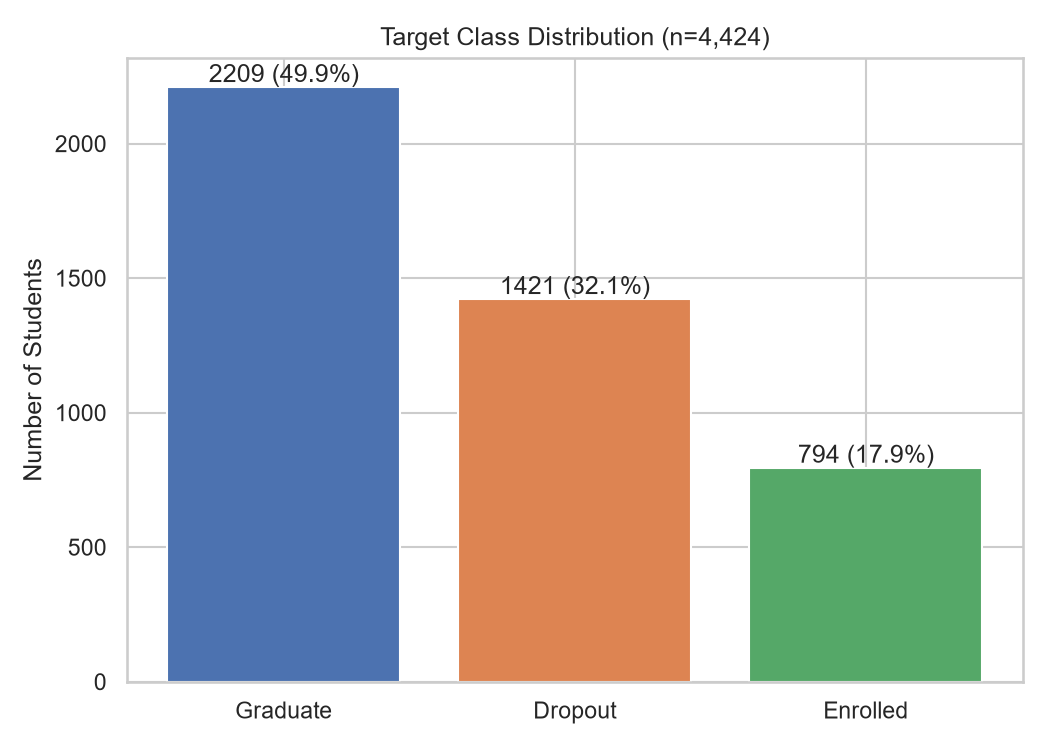
\includegraphics{A_target_distribution.png} etc.
% without repeating the relative path everywhere.
\graphicspath{{../../figures/}}
\usepackage{booktabs}
\usepackage{amsmath}
\usepackage{float}
\usepackage{caption}
\usepackage{xcolor}
\usepackage{hyperref}
\hypersetup{colorlinks=true, linkcolor=blue, citecolor=blue, urlcolor=blue}
\usepackage[round]{natbib}
\setlength{\emergencystretch}{2em}

% Visible TODO marker -- every section file that is not yet filled in uses
% this so it is obvious in the compiled PDF (and in a find-in-file search
% for "\todo") what is still missing. Delete a \todo call once that piece
% is actually written; do not leave stale TODOs in a submitted report.
\newcommand{\todo}[1]{{\color{red}\textbf{[TODO --- #1]}}}

\title{Lab 2: Decision Tree Modeling and Improvement \\ \large Predicting Student Dropout and Academic Success}
\author{Group \todo{GroupID} \\ \todo{Course / instructor}}
\date{\today}

\begin{document}

\maketitle

% Owner: Team lead. Source material: docs/report_draft_g_h.md has a
% ready-made contribution table (Vietnamese) at "Phan J1 -- Bang dong gop
% thanh vien" style rows in docs/02-DATASET-VA-CONG-VIEC.md; the actual
% names/student IDs must come from the real team, not invented here.
%
% Brief requires (Section 3.4.a):
%   - Group name, student IDs, and member list.
%   - Specific contribution of each member.
%
% Also worth double-checking here (see progress/A.md log 2026-08-30):
% one git commit tagged "[C]" (hash 0969118) was actually Role E's work
% under a different git author -- do not credit that commit to C when
% writing the contribution percentages/descriptions below.

\section{Group Introduction}
\label{sec:a}

\textbf{Group 2}

\begin{table}[H]
  \centering
  \caption{Team members and contributions}
  \label{tab:contrib}
  \begin{tabular}{@{}p{2.3cm}p{1.9cm}p{8.2cm}p{2cm}@{}}
    \toprule
    Name & Student ID & Contribution & \% \\
    \midrule
    \vnname{Trần Hoàng Phúc} & 24127505 & Data collection \& description, EDA, data preprocessing pipeline, final results aggregation, wrote Introduction / Dataset Description / Comparison / Conclusion & 100\% \\
    \vnname{Nguyễn Văn Minh} & 24127205 & Baseline model, tree/rule visualization tooling, wrote Baseline Model \& Analysis of the Tree & 100\% \\
    \vnname{Thái Quang Huy} & 24127177 & Cost-complexity pruning (Improvement 1), wrote section f.1 & 100\% \\
    \vnname{Nguyễn Hữu Gia Minh} & 24127078 & Class imbalance handling (Improvement 2), wrote section f.2 & 100\% \\
    \vnname{Mai Phương Thùy} & 24127249 & Feature selection for early warning (Improvement 3), slides, video, references, wrote section f.3 & 100\% \\
    \bottomrule
  \end{tabular}
\end{table}

Each member is credited at 100\% for the section(s) they own, since the
work was divided by section rather than split fractionally across the
whole report.

% Owner: Role A. Translated and adapted from the verified Vietnamese draft
% docs/report_draft_b_c.md (section "b. Introduction"). Every claim in that
% source file was fact-checked against src/data.py, data/raw/data.csv, and
% outputs/results.csv before translation -- see progress/A.md 2026-08-30
% logs for the audit trail. If you edit this file, keep it consistent with
% the source draft or update both.

\section{Introduction}
\label{sec:b}

\subsection{Brief introduction to decision trees}

A decision tree is a supervised learning model used for both classification
and regression tasks. It represents the decision process as a tree
structure: each \emph{internal node} tests one feature (e.g.\ ``Tuition
fees up to date $\le 0.5$?''), each \emph{branch} corresponds to the
outcome of that test, and each \emph{leaf node} assigns a predicted class.

Training a decision tree follows a \textbf{greedy, top-down,
recursive-partitioning} strategy: at each node, the algorithm evaluates
every feature and every possible split threshold, and picks the split that
reduces class \emph{impurity} the most, then repeats recursively on each
resulting subset. Two impurity measures are standard:

\begin{itemize}
  \item \textbf{Entropy / Information Gain}: used by the ID3 algorithm
    \citep{quinlan1986induction}, measuring the information gained by a
    split.
  \item \textbf{Gini impurity}: used by CART \citep{breiman1984classification},
    measuring the probability of misclassification if a label were drawn
    at random from the node's class distribution.
\end{itemize}

The scikit-learn library used in this project implements an optimized
variant of CART \citep{pedregosa2011scikit}; it defaults to Gini but
supports switching to entropy via the \texttt{criterion} parameter.

The \textbf{main strength} of a decision tree compared to ``black-box''
models (neural networks, complex ensembles) is \textbf{interpretability}:
every path from the root to a leaf can be read directly as an
\texttt{IF (condition 1) AND (condition 2) ... THEN (label)} rule, with no
separate explanation technique (SHAP, LIME) required. Once nominal
categories have been encoded, trees also handle the resulting numerical
and indicator features without feature scaling. Both properties are used
directly in Section~\ref{sec:c} below.

The \textbf{main weakness} is a tendency to \textbf{overfit}: an
unconstrained tree keeps splitting until almost every leaf is pure on the
training set, effectively memorizing training noise, which yields very
high training accuracy but a much lower test accuracy
\citep{mitchell1997machine, breiman1984classification}. Section~\ref{sec:d}
shows this pattern directly in the baseline model, which motivates the
pruning improvement in Section~\ref{sec:f}.

\subsection{Objective of the project}

The project applies this theory to a real, socially meaningful problem:
\textbf{predicting whether a student drops out, remains enrolled longer
than expected, or graduates on time}, using real data from 4{,}424
university students in Portugal. Concretely, the group:

\begin{enumerate}
  \item Builds and evaluates an unconstrained baseline decision tree,
    measuring performance with the full set of metrics appropriate for a
    3-class classification problem (Accuracy, Precision, Recall,
    F1-score, ROC-AUC, Confusion Matrix).
  \item Analyzes the baseline tree's structure: what the root split is
    and why the algorithm chose it, whether the tree shows signs of
    overfitting, and extracts concrete decision rules.
  \item Proposes and tests three improvement methods, each targeting a
    different weakness of the baseline:
  \begin{itemize}
    \item \textbf{Pruning} (cost-complexity pruning): trades tree
      complexity for generalization to address overfitting.
    \item \textbf{Class-imbalance handling}
      (\texttt{class\_weight='balanced'}, SMOTE): addresses the model's
      default bias toward the majority class (Graduate). At baseline,
      Enrolled recall (0.3836) is well below Dropout's already-reasonable
      recall (0.6796), so Enrolled is the main target of this improvement.
    \item \textbf{Feature selection for early warning}: addresses a
      practical limitation. The baseline's strongest features are only
      known \emph{after} a semester ends, so the model with the highest
      accuracy is not necessarily the model that can actually be deployed
      for early intervention.
  \end{itemize}
  \item Quantitatively compares all five model configurations and asks
    \textbf{which model suits which application goal}, in line with the
    assignment brief's emphasis on explaining how the tree is built, how
    it behaves, and why each improvement helps or does not, rather than
    only reporting a final accuracy score.
\end{enumerate}

% Final section; CSV-derived claims and published metadata were audited
% separately so their evidence bases remain explicit.

\section{Dataset Description}
\label{sec:c}

\subsection{Data source}

The group uses the \textbf{``Predict Students' Dropout and Academic
Success''} dataset from the UCI Machine Learning Repository (ID~=~697),
published by Realinho, Vieira Martins, Machado, and Baptista
\citep{realinho2021dataset}, licensed CC~BY~4.0. The dataset is described
in detail in the accompanying paper \citep{realinho2022predicting}.

The data was collected at \textbf{Instituto Polit\'ecnico de Portalegre},
Portugal, spanning \textbf{17 undergraduate degree programs} (Agronomy,
Design, Nursing, Journalism and Communication, Management, Social
Service, Biofuel Production Technologies, Informatics Engineering, etc.),
academic years \textbf{2008/09 to 2018/19}. It combines information from
several administrative sources at enrollment time (admission records,
socio-economic data) with academic outcomes at the end of each of the
first two semesters \citep[Section~2, ``Data Description'']{realinho2022predicting}.

\subsection{Dataset description --- numbers confirmed from actual data}

The group did not copy figures from the UCI metadata page; instead it
directly inspected the raw dataset to confirm:

\begin{itemize}
  \item The raw file contains \textbf{4,424 rows and 37 columns}: 4{,}424
    samples (students), 36 features plus 1 label column \texttt{Target}.
  \item There are \textbf{zero} missing values across the whole dataset
    (the authors pre-cleaned the data).
  \item \textbf{Notable finding:} the UCI page lists 36 features, but
    Table~1 of the original paper lists only 34. Cross-checking the
    actual column list against that table, the discrepancy is exactly
    two columns: \texttt{Previous qualification (grade)} and
    \texttt{Admission grade}, both present in the released CSV but absent
    from the paper's table. That discrepancy is only visible by reading
    the actual column list, not by copying the metadata page.
\end{itemize}

The 36 features fall into six groups by nature: demographics (6 columns,
e.g.\ Gender, Age at enrollment), socio-economic status (8 columns, e.g.\
Tuition fees up to date, Scholarship holder), macroeconomics (3 columns:
Unemployment rate, Inflation rate, GDP), academic background at
enrollment (7 columns, e.g.\ Course, Admission grade), first-semester
outcomes (6 columns), and second-semester outcomes (6 columns).

\textbf{Target variable} has 3 classes, moderately imbalanced:

\begin{table}[H]
  \centering
  \caption{Target class distribution (n = 4{,}424)}
  \begin{tabular}{@{}lrrp{6cm}@{}}
    \toprule
    Class & Count & \% & Meaning \\
    \midrule
    Graduate & 2{,}209 & 49.9\% & Graduated on the standard timeline (3 years; 4 for Nursing) \\
    Dropout  & 1{,}421 & 32.1\% & Dropped out \\
    Enrolled & 794     & 17.9\% & Still enrolled past the standard timeline \\
    \bottomrule
  \end{tabular}
  \\[0.3em]
  \footnotesize Percentages are rounded to one decimal place and therefore
  sum to 99.9\% rather than 100\%; the unrounded values (49.93\%, 32.12\%,
  17.95\%) sum to 100\%.
\end{table}

\textbf{Enrolled} is both the minority class and the hardest to classify:
across every model configuration compared in Section~\ref{sec:g}, its
recall is the lowest of the three classes (e.g.\ 0.3836 for the baseline
M0), which is why the class-imbalance improvement (Section~\ref{sec:f},
f.2) targets this class.

\begin{figure}[H]
  \centering
  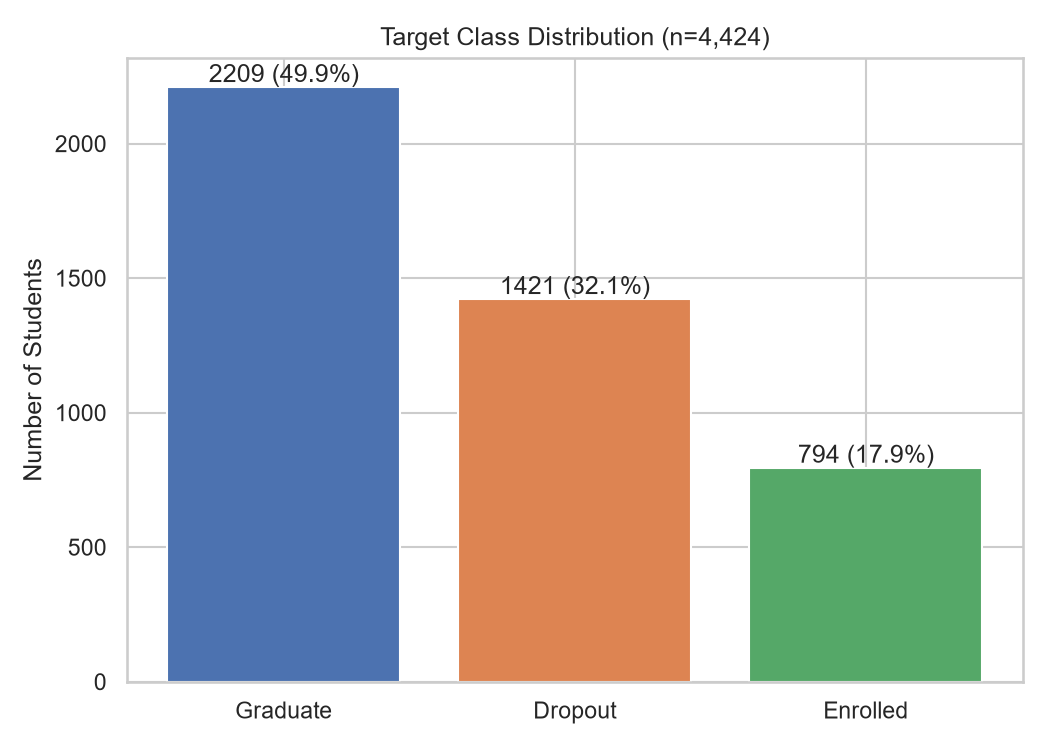
\includegraphics[width=0.7\textwidth]{A_target_distribution.png}
  \caption{Target class distribution (n = 4{,}424).}
  \label{fig:c1}
\end{figure}

Several of the observations below refer to how strongly a feature drives
the baseline decision tree's actual splits, measured by Gini importance
(the total reduction in class impurity attributed to that feature across
the whole tree, described further in Section~\ref{sec:d}). Table~\ref{tab:c-importance}
lists the top 10 features by this measure, plus one lower-ranked feature
included for contrast with the discussion below.

\begin{table}[H]
  \centering
  \caption{Top-10 features by Gini importance in the baseline tree (M0), plus one feature shown for contrast}
  \label{tab:c-importance}
  \begin{tabular}{@{}rlr@{}}
    \toprule
    Rank & Feature & Gini importance \\
    \midrule
    1  & Curricular units 2nd sem (approved)    & 0.340 \\
    2  & Curricular units 2nd sem (grade)       & 0.045 \\
    3  & Tuition fees up to date                & 0.045 \\
    4  & Curricular units 2nd sem (enrolled)    & 0.045 \\
    5  & Admission grade                        & 0.044 \\
    6  & Course                                 & 0.044 \\
    7  & Curricular units 1st sem (evaluations) & 0.034 \\
    8  & Previous qualification (grade)         & 0.031 \\
    9  & Curricular units 1st sem (approved)    & 0.029 \\
    10 & Mother's occupation                    & 0.028 \\
    \multicolumn{3}{c}{\ldots} \\
    24 & Scholarship holder                     & 0.010 \\
    \bottomrule
  \end{tabular}
\end{table}

Descriptive statistics from exploratory data analysis illustrate how
strongly some features relate to the target: among
students who had \textbf{not paid tuition on time}, 86\% ended up in the
Dropout class, versus 25\% Dropout / 56\% Graduate among students who had
paid on time. Students with a \textbf{scholarship} have a Dropout rate
26.5 percentage points lower than those without (12.2\% vs.\ 38.7\%);
their rate is about one-third as high.

\begin{figure}[H]
  \centering
  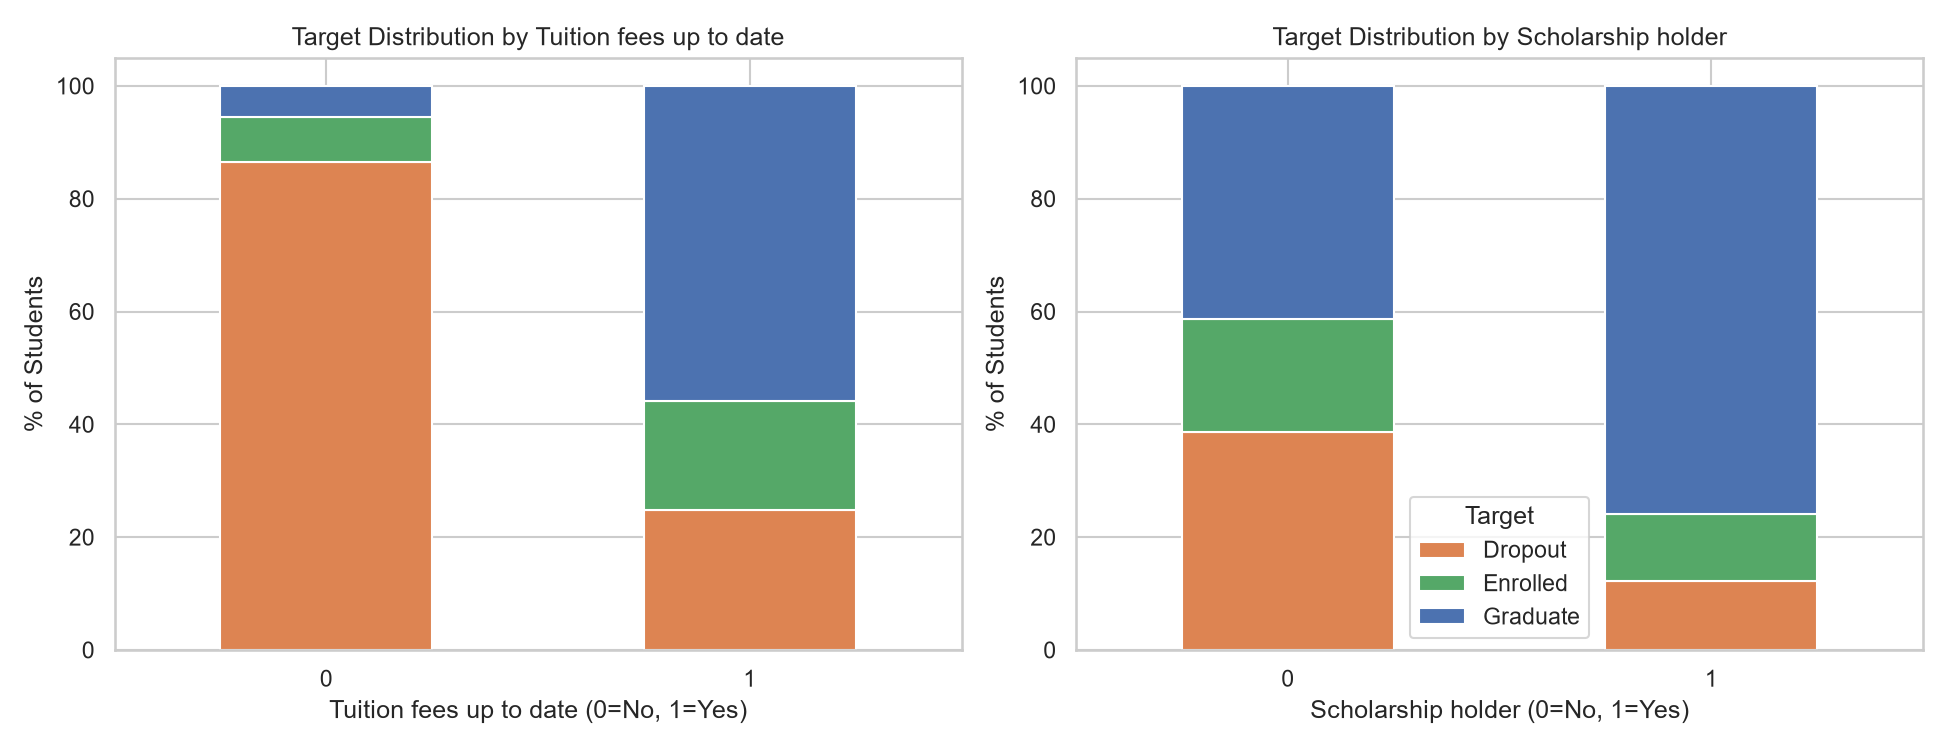
\includegraphics[width=0.9\textwidth]{A_tuition_scholarship_vs_target.png}
  \caption{Target distribution split by \texttt{Tuition fees up to date}
    (left) and \texttt{Scholarship holder} (right).}
  \label{fig:c2}
\end{figure}

\texttt{Tuition fees up to date} is among the top-5 features by
permutation importance in the original paper \citep{realinho2022predicting},
and is also rank~3 in Table~\ref{tab:c-importance}: the two ways of
measuring importance agree here. \texttt{Scholarship holder} is a more
subtle case: it is \textbf{not} in the top-5 of either the paper or
Table~\ref{tab:c-importance} (rank~24), even though its
percentage-of-target chart above looks just as striking as tuition's. A
large gap in a simple percentage-of-target chart does not automatically
mean a feature drives an important tree split once it sits alongside
stronger, possibly overlapping features such as \texttt{Tuition fees up
to date}; the tree may instead be extracting the same signal from that
stronger correlate.

By program of study, the two lowest-graduation programs are course code
33 (Biofuel Production Technologies, $n=12$: 8 Dropout, 3 Enrolled, and
1 Graduate; 66.7\% Dropout) and course
code 9119 (Informatics Engineering, $n=170$, 54.1\% Dropout). Only
\textbf{8.3\% and 8.2\%} of their students graduate respectively, versus
the dataset average of 49.9\%. Course 33's rate is based on a very small
sample ($n=12$) and is not evidence of a stable program-level effect. The
two highest-graduation programs are course code 9238 (Social Service,
$n=355$, 69.9\% Graduate) and course code 9500 (Nursing, $n=766$, 71.5\%
Graduate), with the lowest Dropout rates (18.3\% and 15.4\%).

\begin{figure}[H]
  \centering
  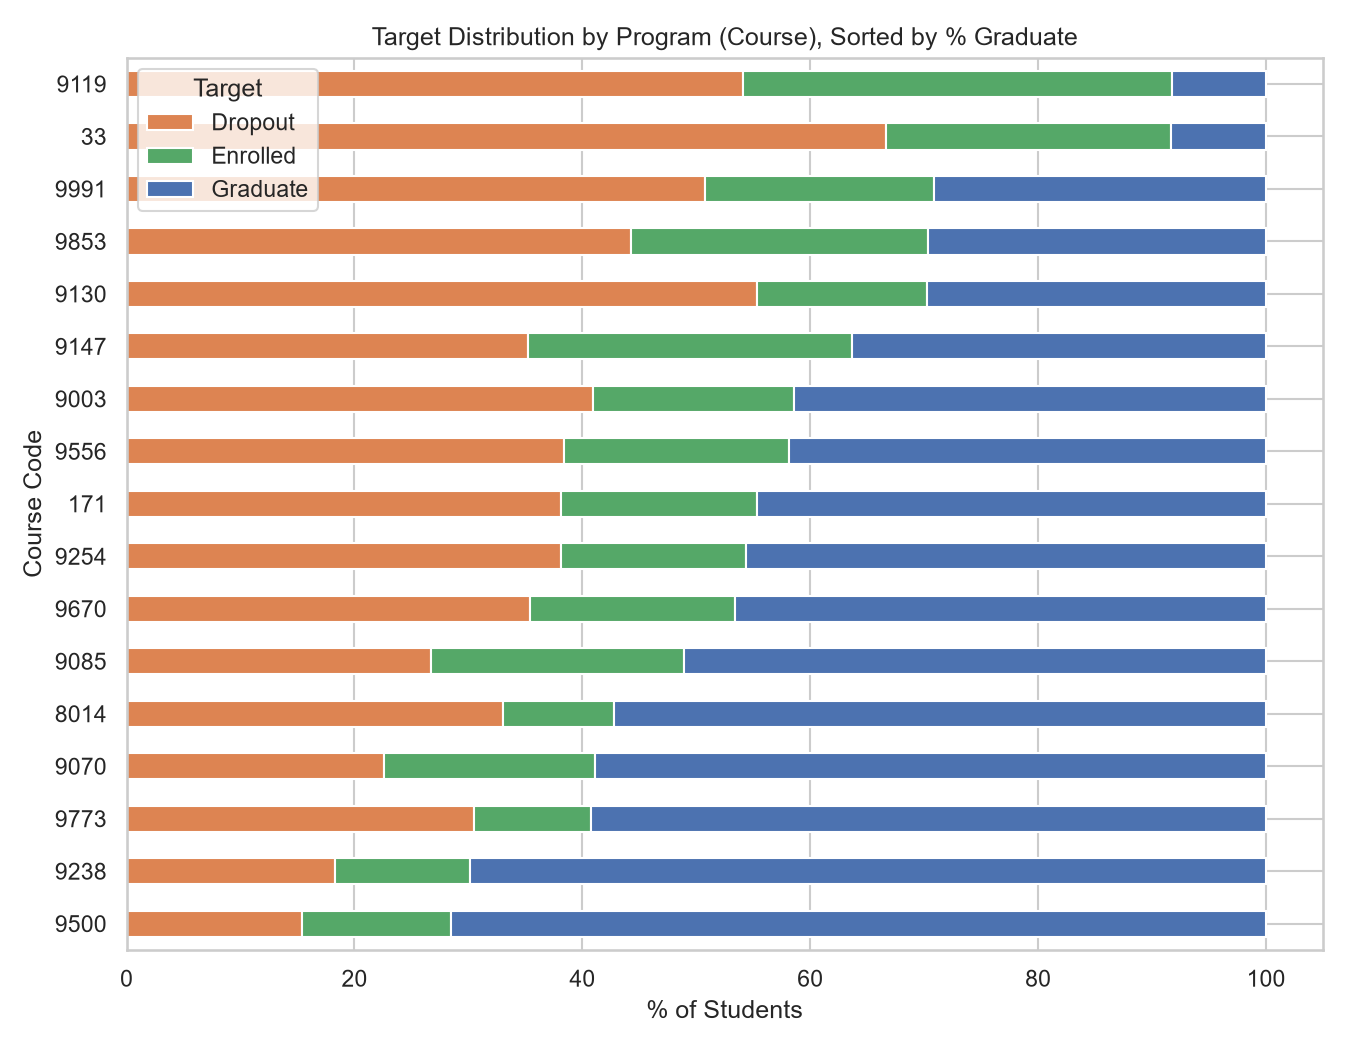
\includegraphics[width=0.85\textwidth]{A_target_by_course.png}
  \caption{17 programs sorted by increasing Graduate rate.}
  \label{fig:c3}
\end{figure}

The original paper ranks \texttt{Course} in its top-5 features by
permutation importance \citep{realinho2022predicting}; in
Table~\ref{tab:c-importance}, \texttt{Course} ranks 6th, close to top-5
either way. Under the study's feature-availability assumption, it is treated
as available at enrollment and therefore retained in M3
(Section~\ref{sec:f}, f.3).

The strongest single predictor in the whole dataset, by contrast, is
only known once a semester has actually happened:

\begin{figure}[H]
  \centering
  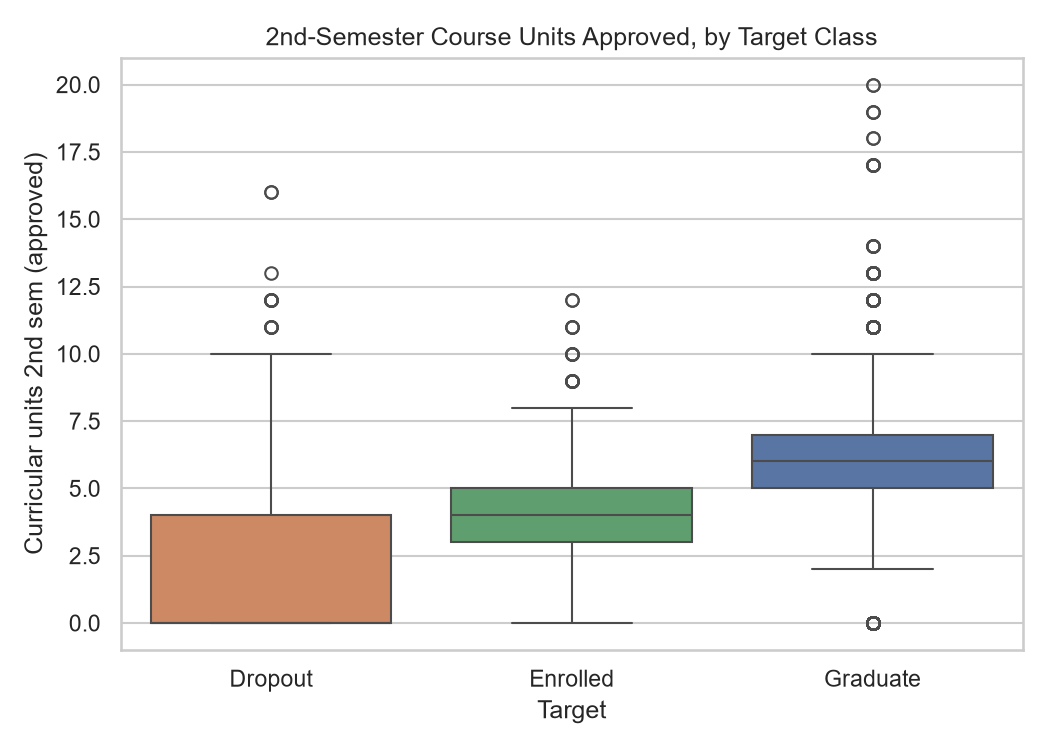
\includegraphics[width=0.7\textwidth]{A_curricular_units_2nd_sem_by_target.png}
  \caption{\texttt{Curricular units 2nd sem (approved)} by Target class.}
  \label{fig:c4}
\end{figure}

Median values are 0 for Dropout, 4 for Enrolled, and 6 for Graduate. This
is the single most important feature in Table~\ref{tab:c-importance}
(rank~1, importance 0.340, more than the sum of ranks 2--5 combined), but
it is defined as a second-semester outcome and is therefore excluded from M3.

\subsection{Preprocessing performed}

All preprocessing logic is implemented in a single shared pipeline, used
by the whole team so every model is evaluated on the exact same
train/test split.

\begin{enumerate}
  \item \textbf{No missing-value handling needed}: the dataset is
    already clean at the source (0 missing values).
  \item \textbf{Re-encoding categorical columns stored as integers.} Many
    columns are integer codes for unordered categories (e.g.\
    \texttt{Course} code 33 = Biofuel Production Technologies, code 9500
    = Nursing \citep[Variables Table, row ``Course'']{realinho2021dataset};
    these codes carry no ordinal relationship). Left as-is,
    scikit-learn would treat them as continuous and produce meaningless
    splits like \texttt{Course} $\le$ 8.5. The group used a mixed
    strategy:
  \begin{itemize}
    \item \textbf{One-hot encode} the 4 low-cardinality columns:
      \texttt{Marital Status} (6), \texttt{Application mode} (18),
      \texttt{Course} (17), \texttt{Previous qualification} (17), so
      each split reads as a clear yes/no question (e.g.\ ``is this the
      Nursing program?'').
    \item \textbf{Keep the raw integer code} for high-cardinality
      columns: the mother's and father's occupations (32/46 values),
      the mother's and father's qualifications (29/34 values), and
      \texttt{Nacionality} (21 values). This was a pragmatic choice to
      limit the number of sparse indicators. It imposes an artificial
      order on nominal codes, so thresholds on these columns are an
      acknowledged representation limitation and require cautious
      interpretation.
    \item After this step the feature count grows from 36 to
      \textbf{90} columns.
  \end{itemize}
  \item \textbf{No feature scaling.} A decision tree splits on a
    threshold of one feature at a time, not on distances between data
    points as KNN or linear regression do, so it is invariant to any
    monotonic per-column transform such as scaling. Adding
    \texttt{StandardScaler}/\texttt{MinMaxScaler} here would be
    redundant and would not change the learned tree structure at all.
  \item \textbf{Stratified train/test split}: 80\%/20\%, stratified by
    class to preserve the $\approx$50/32/18 class ratio in both sets.
    This guarantees that both partitions retain the observed class
    proportions. A fixed random seed is used so all five models in the
    project are evaluated on the exact same split.
\end{enumerate}

After preprocessing: \textbf{3{,}539 training samples / 885 test
samples}, each with 90 numeric features, ready to feed directly into a
decision tree classifier.

\subsection{Multicollinearity among features}

\begin{figure}[H]
  \centering
  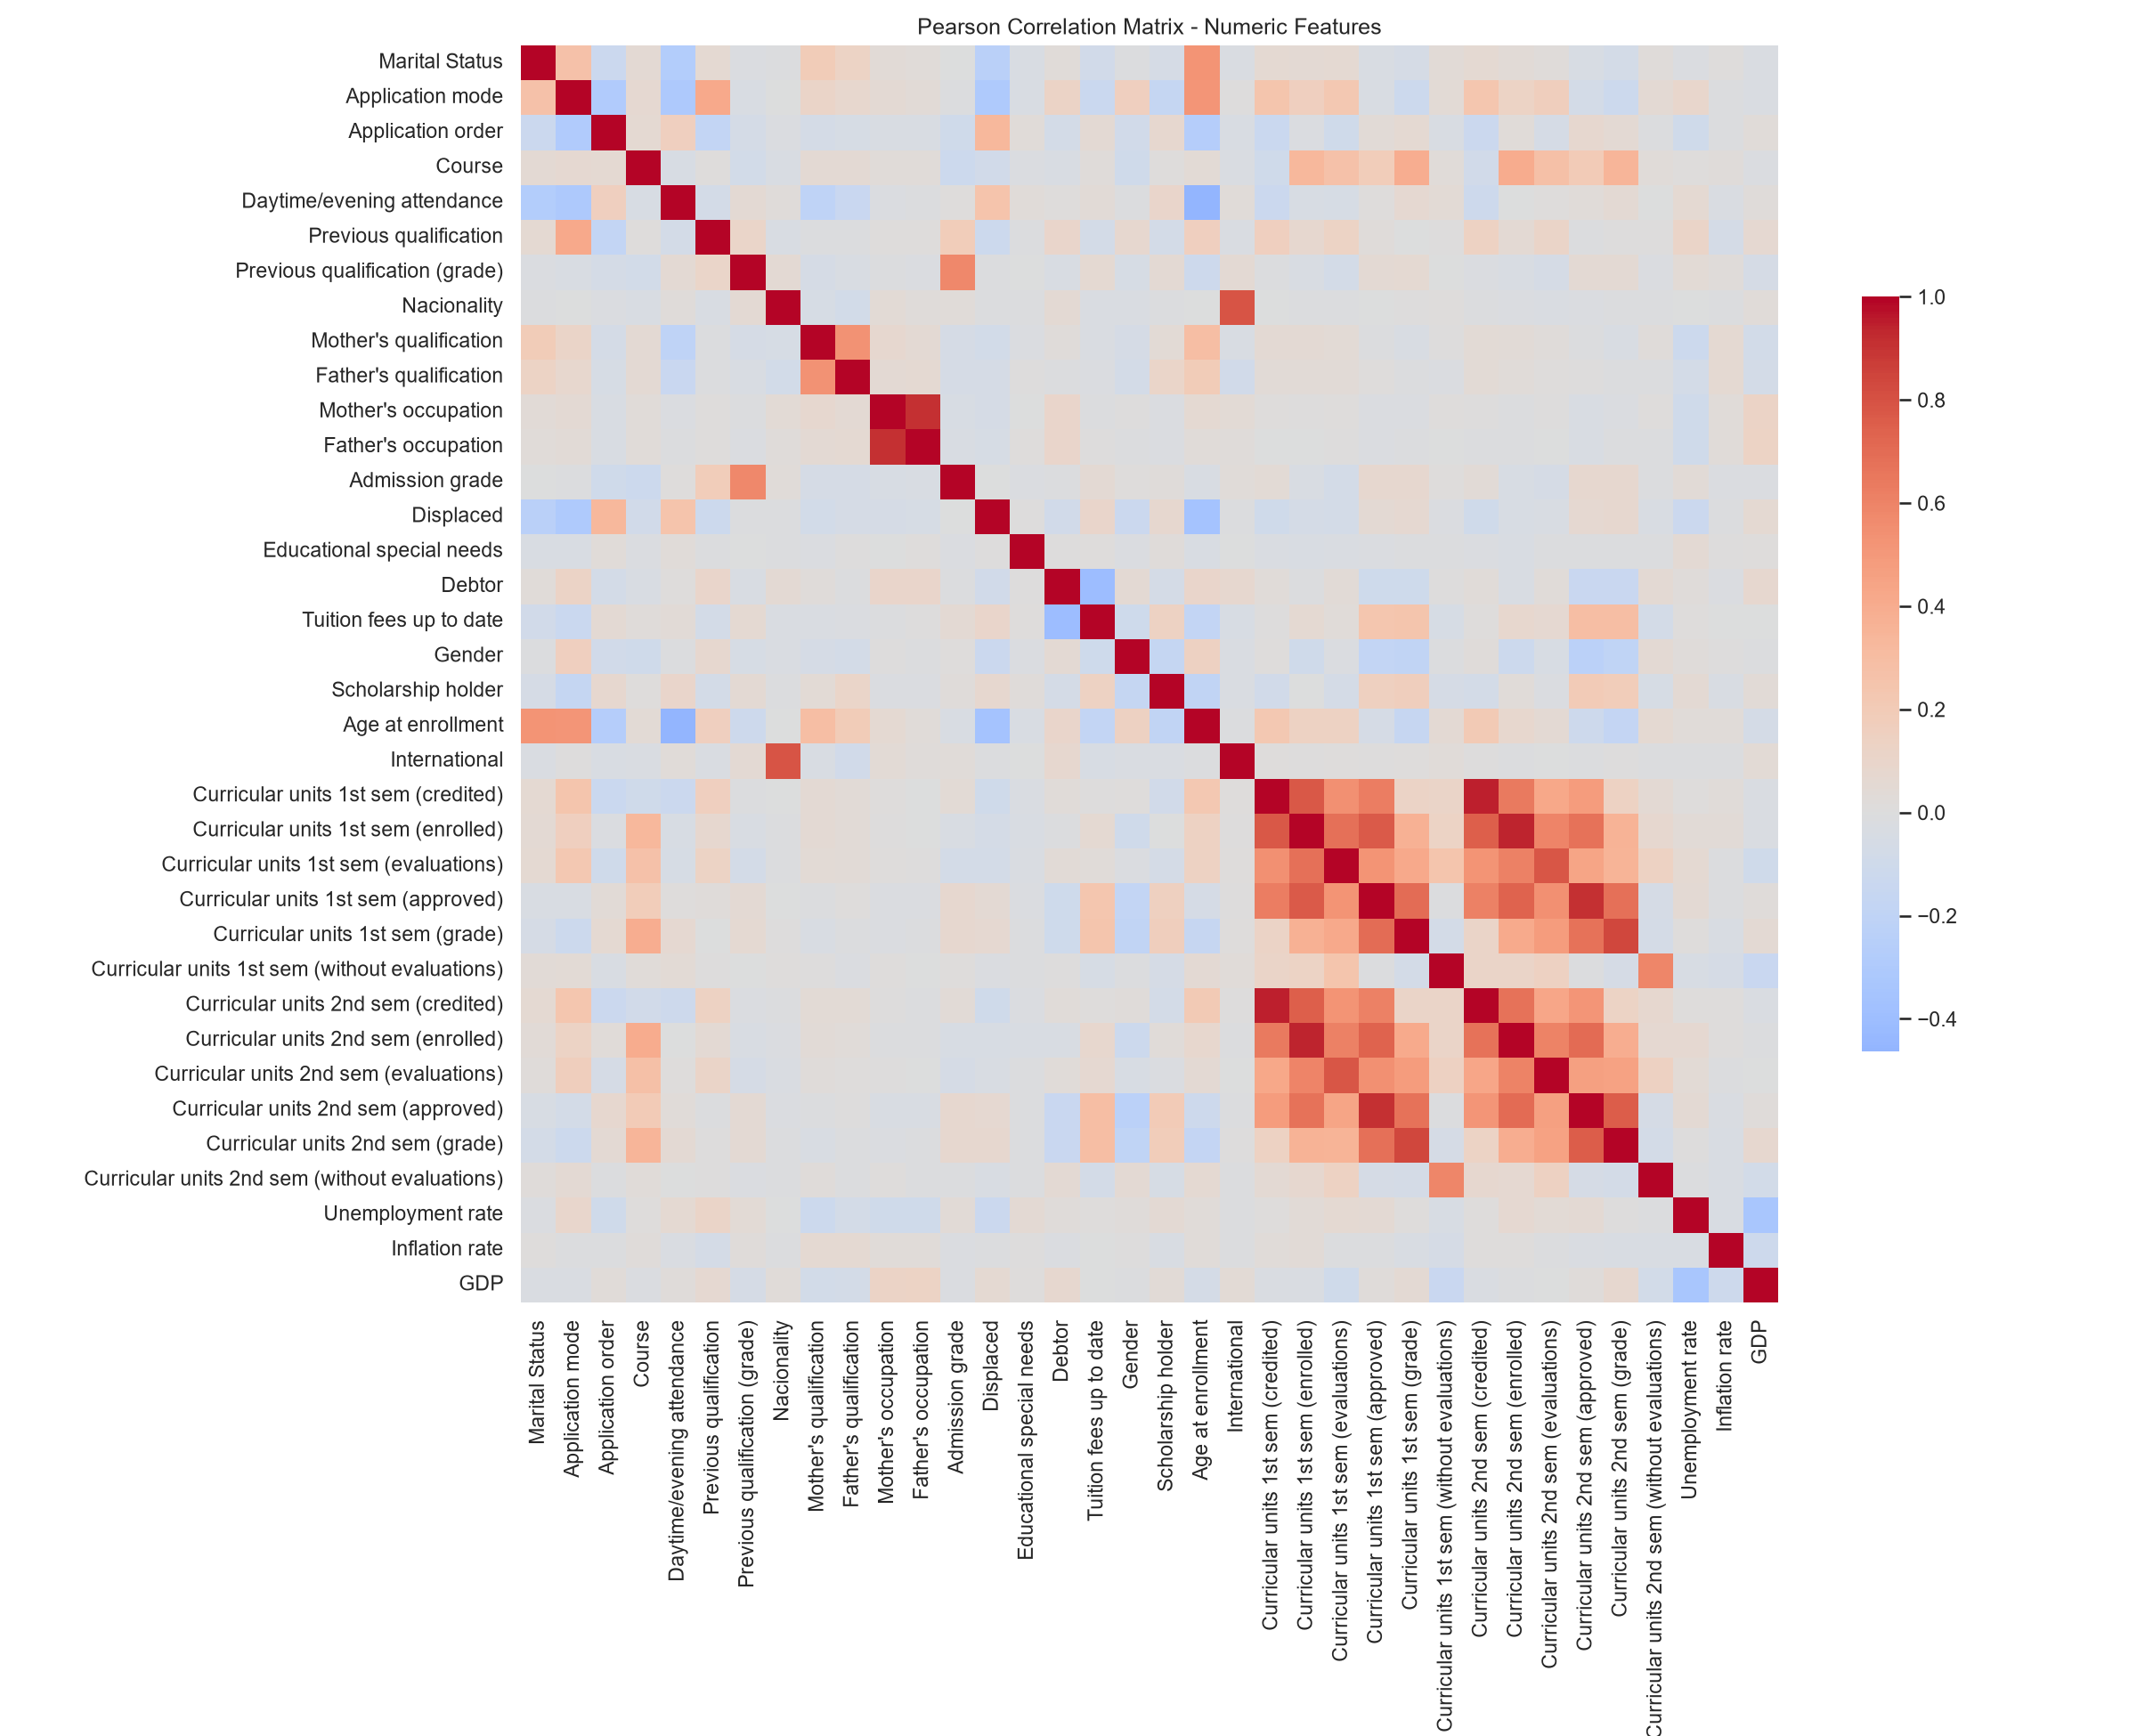
\includegraphics[width=\textwidth]{A_correlation_heatmap.png}
  \caption{Pearson correlation heatmap across all numeric features.}
  \label{fig:c5}
\end{figure}

The heatmap's colors show the overall pattern, but individual cell
values are not printed on a 36$\times$36 grid; Table~\ref{tab:c-corr}
lists the exact values for the pairs discussed here so they can be
checked directly.

\begin{table}[H]
  \centering
  \caption{Highest Pearson correlations in the dataset}
  \label{tab:c-corr}
  \begin{tabular}{@{}llr@{}}
    \toprule
    Feature & Correlated with & $r$ \\
    \midrule
    Curricular units 1st sem (credited) & Curricular units 2nd sem (credited) & 0.945 \\
    Curricular units 1st sem (enrolled) & Curricular units 2nd sem (enrolled) & 0.943 \\
    Mother's occupation                 & Father's occupation                 & 0.910 \\
    Curricular units 1st sem (approved) & Curricular units 2nd sem (approved) & 0.904 \\
    Nacionality                         & International                       & 0.791 \\
    \bottomrule
  \end{tabular}
\end{table}

The three highest-correlation pairs in the whole dataset are
\texttt{1st sem credited} $\leftrightarrow$ \texttt{2nd sem credited},
\texttt{1st sem enrolled} $\leftrightarrow$ \texttt{2nd sem enrolled},
and \textbf{\texttt{Mother's occupation} $\leftrightarrow$
\texttt{Father's occupation}}, which is \emph{higher} than the
semester-approved pair (\texttt{1st/2nd sem approved}). The pair
\texttt{Nacionality} $\leftrightarrow$ \texttt{International} is still a
high correlation (international students almost always have a
non-Portuguese \texttt{Nacionality} code), but lower than the four
pairs above.

A decision tree is not as sensitive to multicollinearity as linear
regression (it does not need redundant features removed to converge),
but multicollinearity still splits feature importance across correlated
columns and can make the tree structure less stable across samples. These
correlations therefore provide diagnostic context, but they are not the
selection rule for M3. The canonical early-warning experiment removes
exactly the 12 semester-outcome columns under the feature-availability
assumption stated in Section~\ref{sec:f3}, while retaining both \texttt{Nacionality} and
\texttt{International} so that feature timing is the only intentional
difference from M0.

\subsection{Why this dataset is appropriate for decision tree modeling}

\begin{enumerate}
  \item \textbf{Features have clear, real-world semantics} (tuition,
    scholarship, semester outcomes, program of study, \ldots), so every
    split translates into an ordinary sentence. This plays directly to a
    decision tree's interpretability strength, in a way that image or
    text features cannot match as easily.
  \item \textbf{A mix of categorical and numerical features}: after
    nominal categories are encoded, the tree handles the resulting
    numerical and indicator columns without scaling, unlike KNN and many
    linear-model workflows, where feature scale directly affects
    distances or optimization.
  \item \textbf{A genuine class imbalance} (50\%/32\%/18\%): creates a
    realistic scenario for applying and comparing imbalance-handling
    techniques, one of the improvement directions the brief itself
    suggests (Section 3.2.d, ``Handling class imbalance'').
  \item \textbf{Documented feature families support a timing experiment}:
    the published documentation distinguishes semester outcomes from
    enrollment-related data. The project therefore evaluates an early-warning
    exclusion rule, while treating the exact availability of every retained
    field as an assumption to be verified from a data dictionary and snapshot
    timestamps before deployment.
  \item \textbf{No missing values}: lets the group spend its time on
    analysis and interpretation instead of data cleaning, matching the
    brief's own emphasis on clearly explaining how the tree is built and
    why the improvements help, beyond simply running a ready-made model.
\end{enumerate}

\subsection{Ethical note}

The dataset contains sensitive variables: gender, nationality, marital
status, and parents' education/occupation. Any tree splits on these
variables only reflect \textbf{correlations observed in one Portuguese
institution's sample from academic years 2008/09--2018/19
\citep[Section~2]{realinho2022predicting}}, not causal relationships, and
should not be used as grounds for any discriminatory policy toward
students in practice.

% Owner: Role B. NOT translated yet -- this is a structural skeleton only.
%
% Source material (Vietnamese, already fact-checked -- see
% progress/A.md 2026-08-30 audit: 0 errors found in this file out of
% ~40 checked numeric claims): docs/report_draft_d_e.md, top part
% (headed "# d. Baseline Model", down to "## Kiem tra phu Gini va Entropy").
% Translate/adapt that verified content into English below -- do not
% re-derive numbers from scratch, they were already independently
% re-verified by a fresh retrain during the audit.
%
% Brief requires (Section 3.4.d):
%   - Description of the initial decision tree model.
%   - Training and testing procedure.
%   - Resulting tree figure or visualization.
%   - Accuracy and error rate of the baseline model.
%
% Figures already committed and ready to reference (do not rename):
%   figures/B_tree_M0_full.png   -- full tree (illustrates overfitting)
%   figures/B_tree_M0_top3.png   -- max_depth=3 view (readable)
%   figures/B_cm_M0.png          -- confusion matrix

\section{d. Baseline Model}
\label{sec:d}

\subsection{Model description and training procedure}

\todo{Describe the unconstrained Gini baseline (random seed 42) and the shared fixed, stratified split: 3,539 training rows and 885 test rows.}

\subsection{Resulting tree}

\begin{figure}[H]
  \centering
  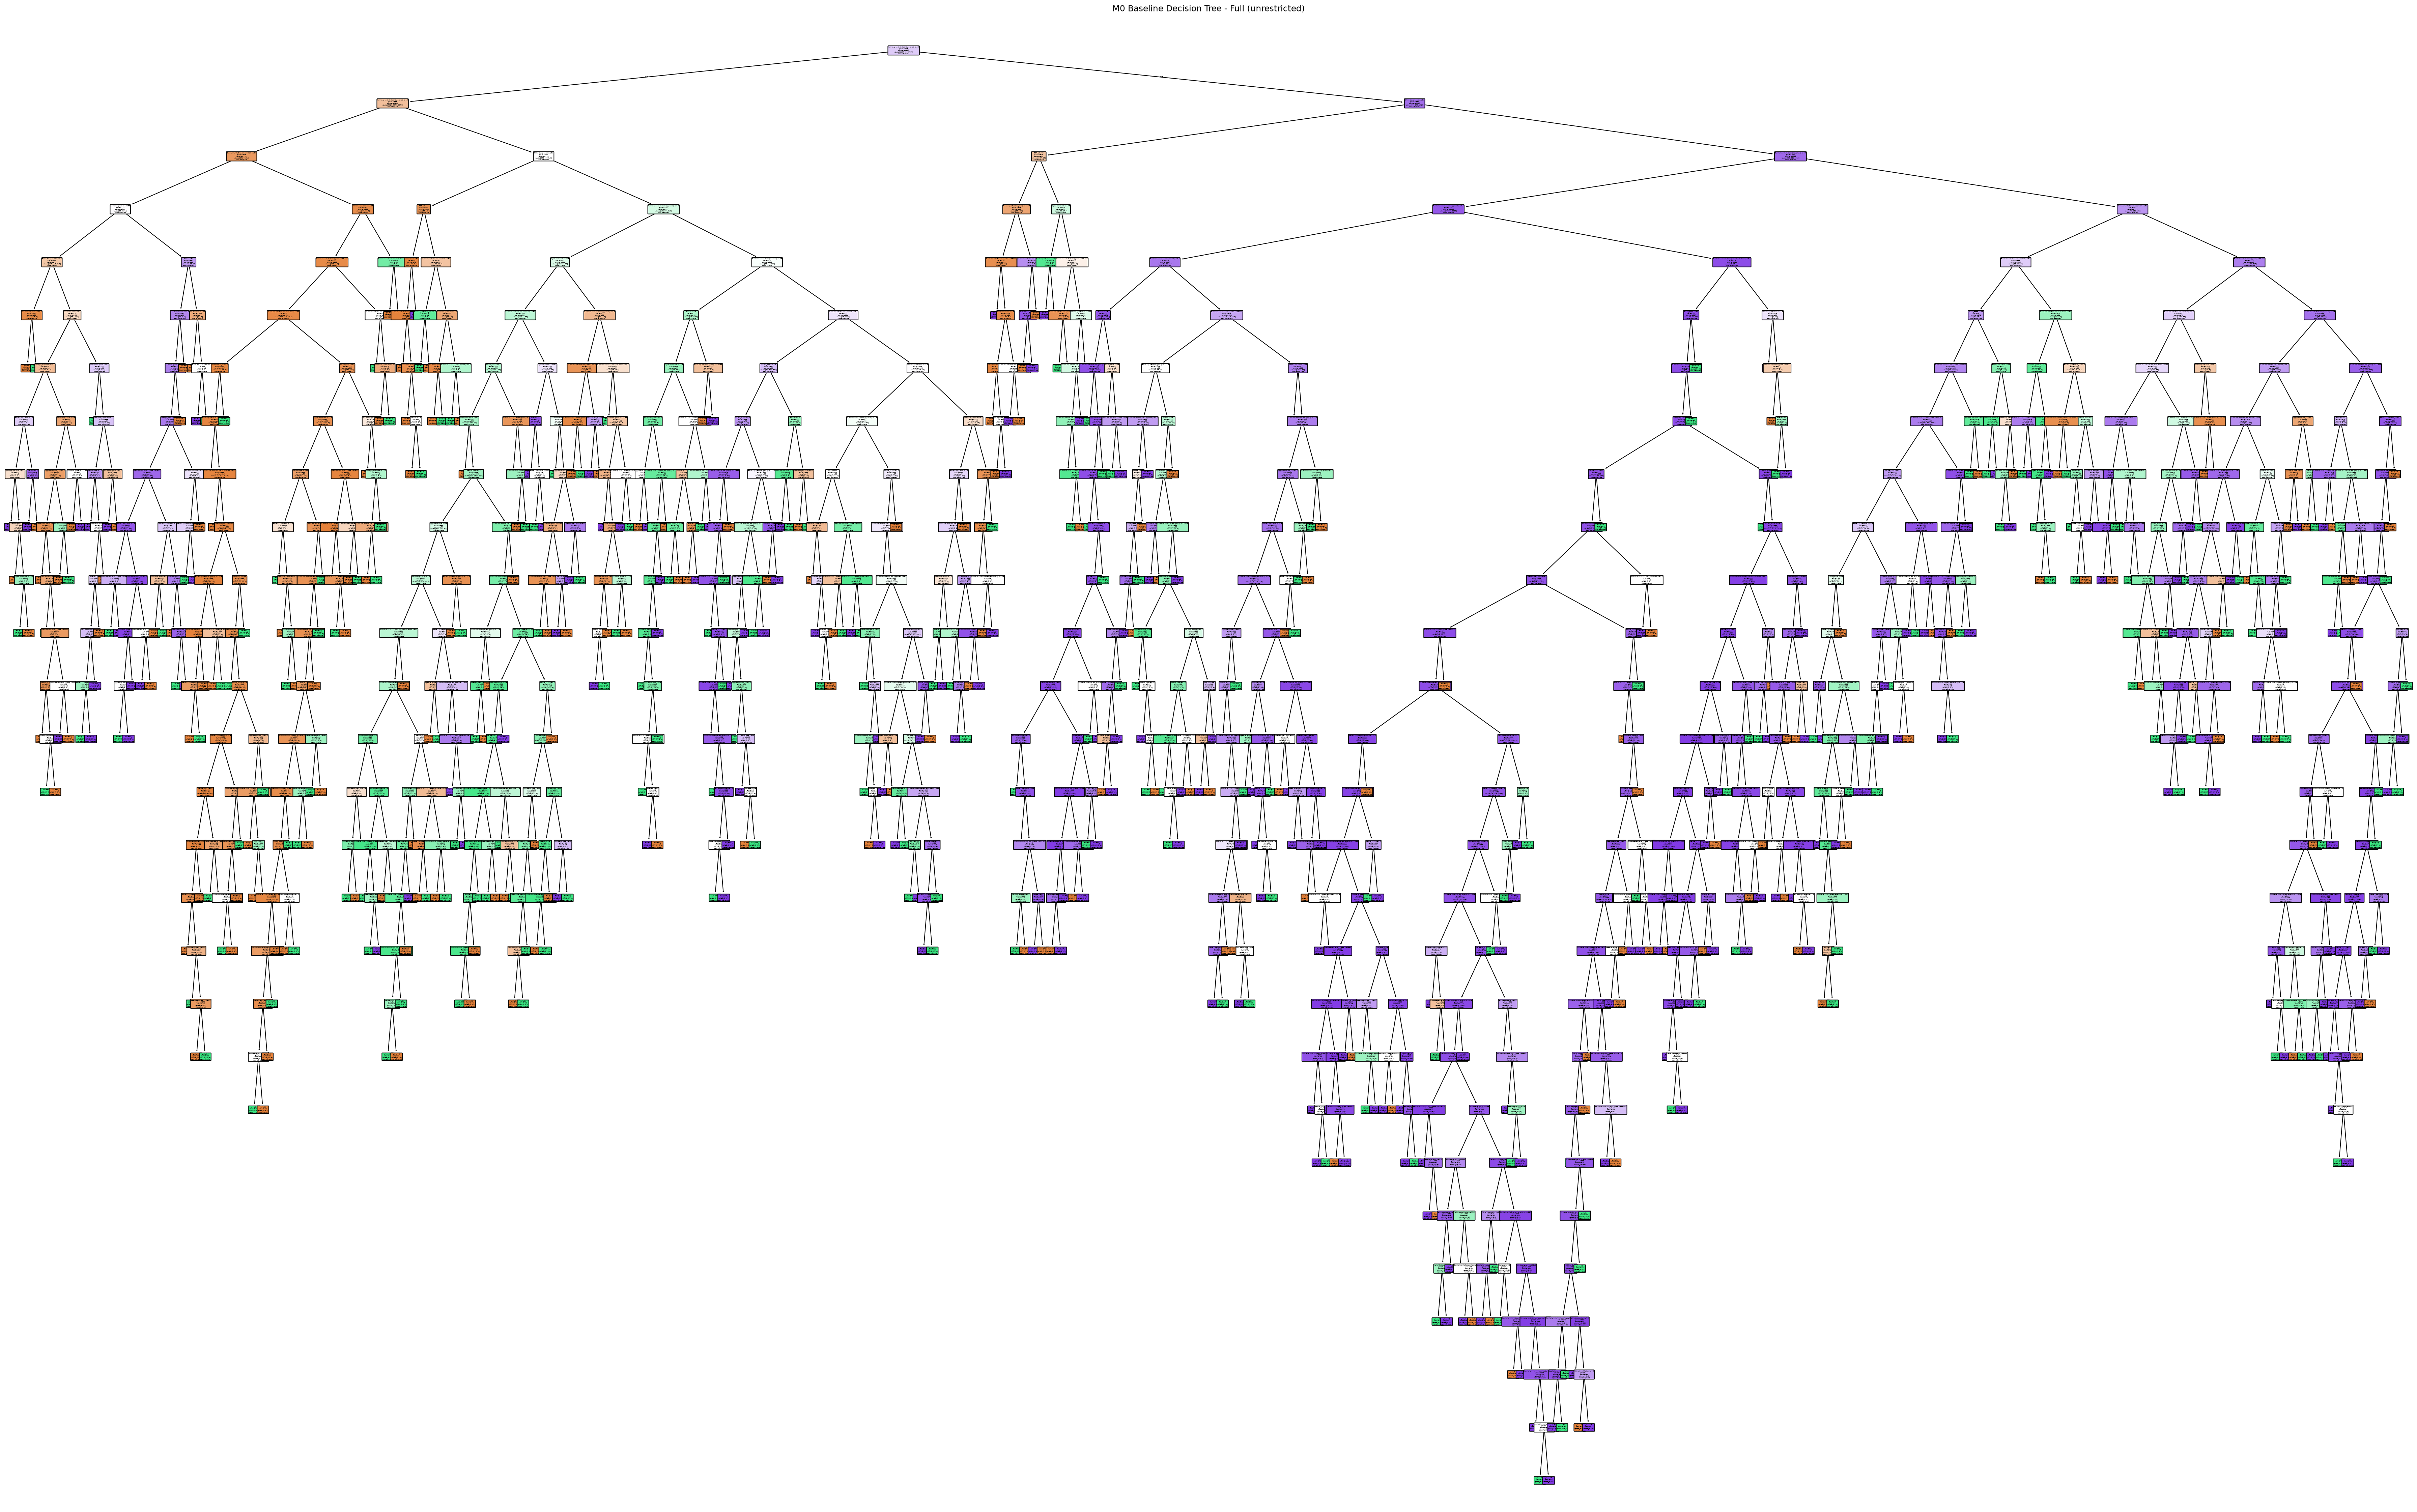
\includegraphics[width=\textwidth]{B_tree_M0_full.png}
  \caption{\todo{Caption: full M0 tree -- state node/leaf count and what it illustrates (overfitting).}}
  \label{fig:d1}
\end{figure}

\begin{figure}[H]
  \centering
  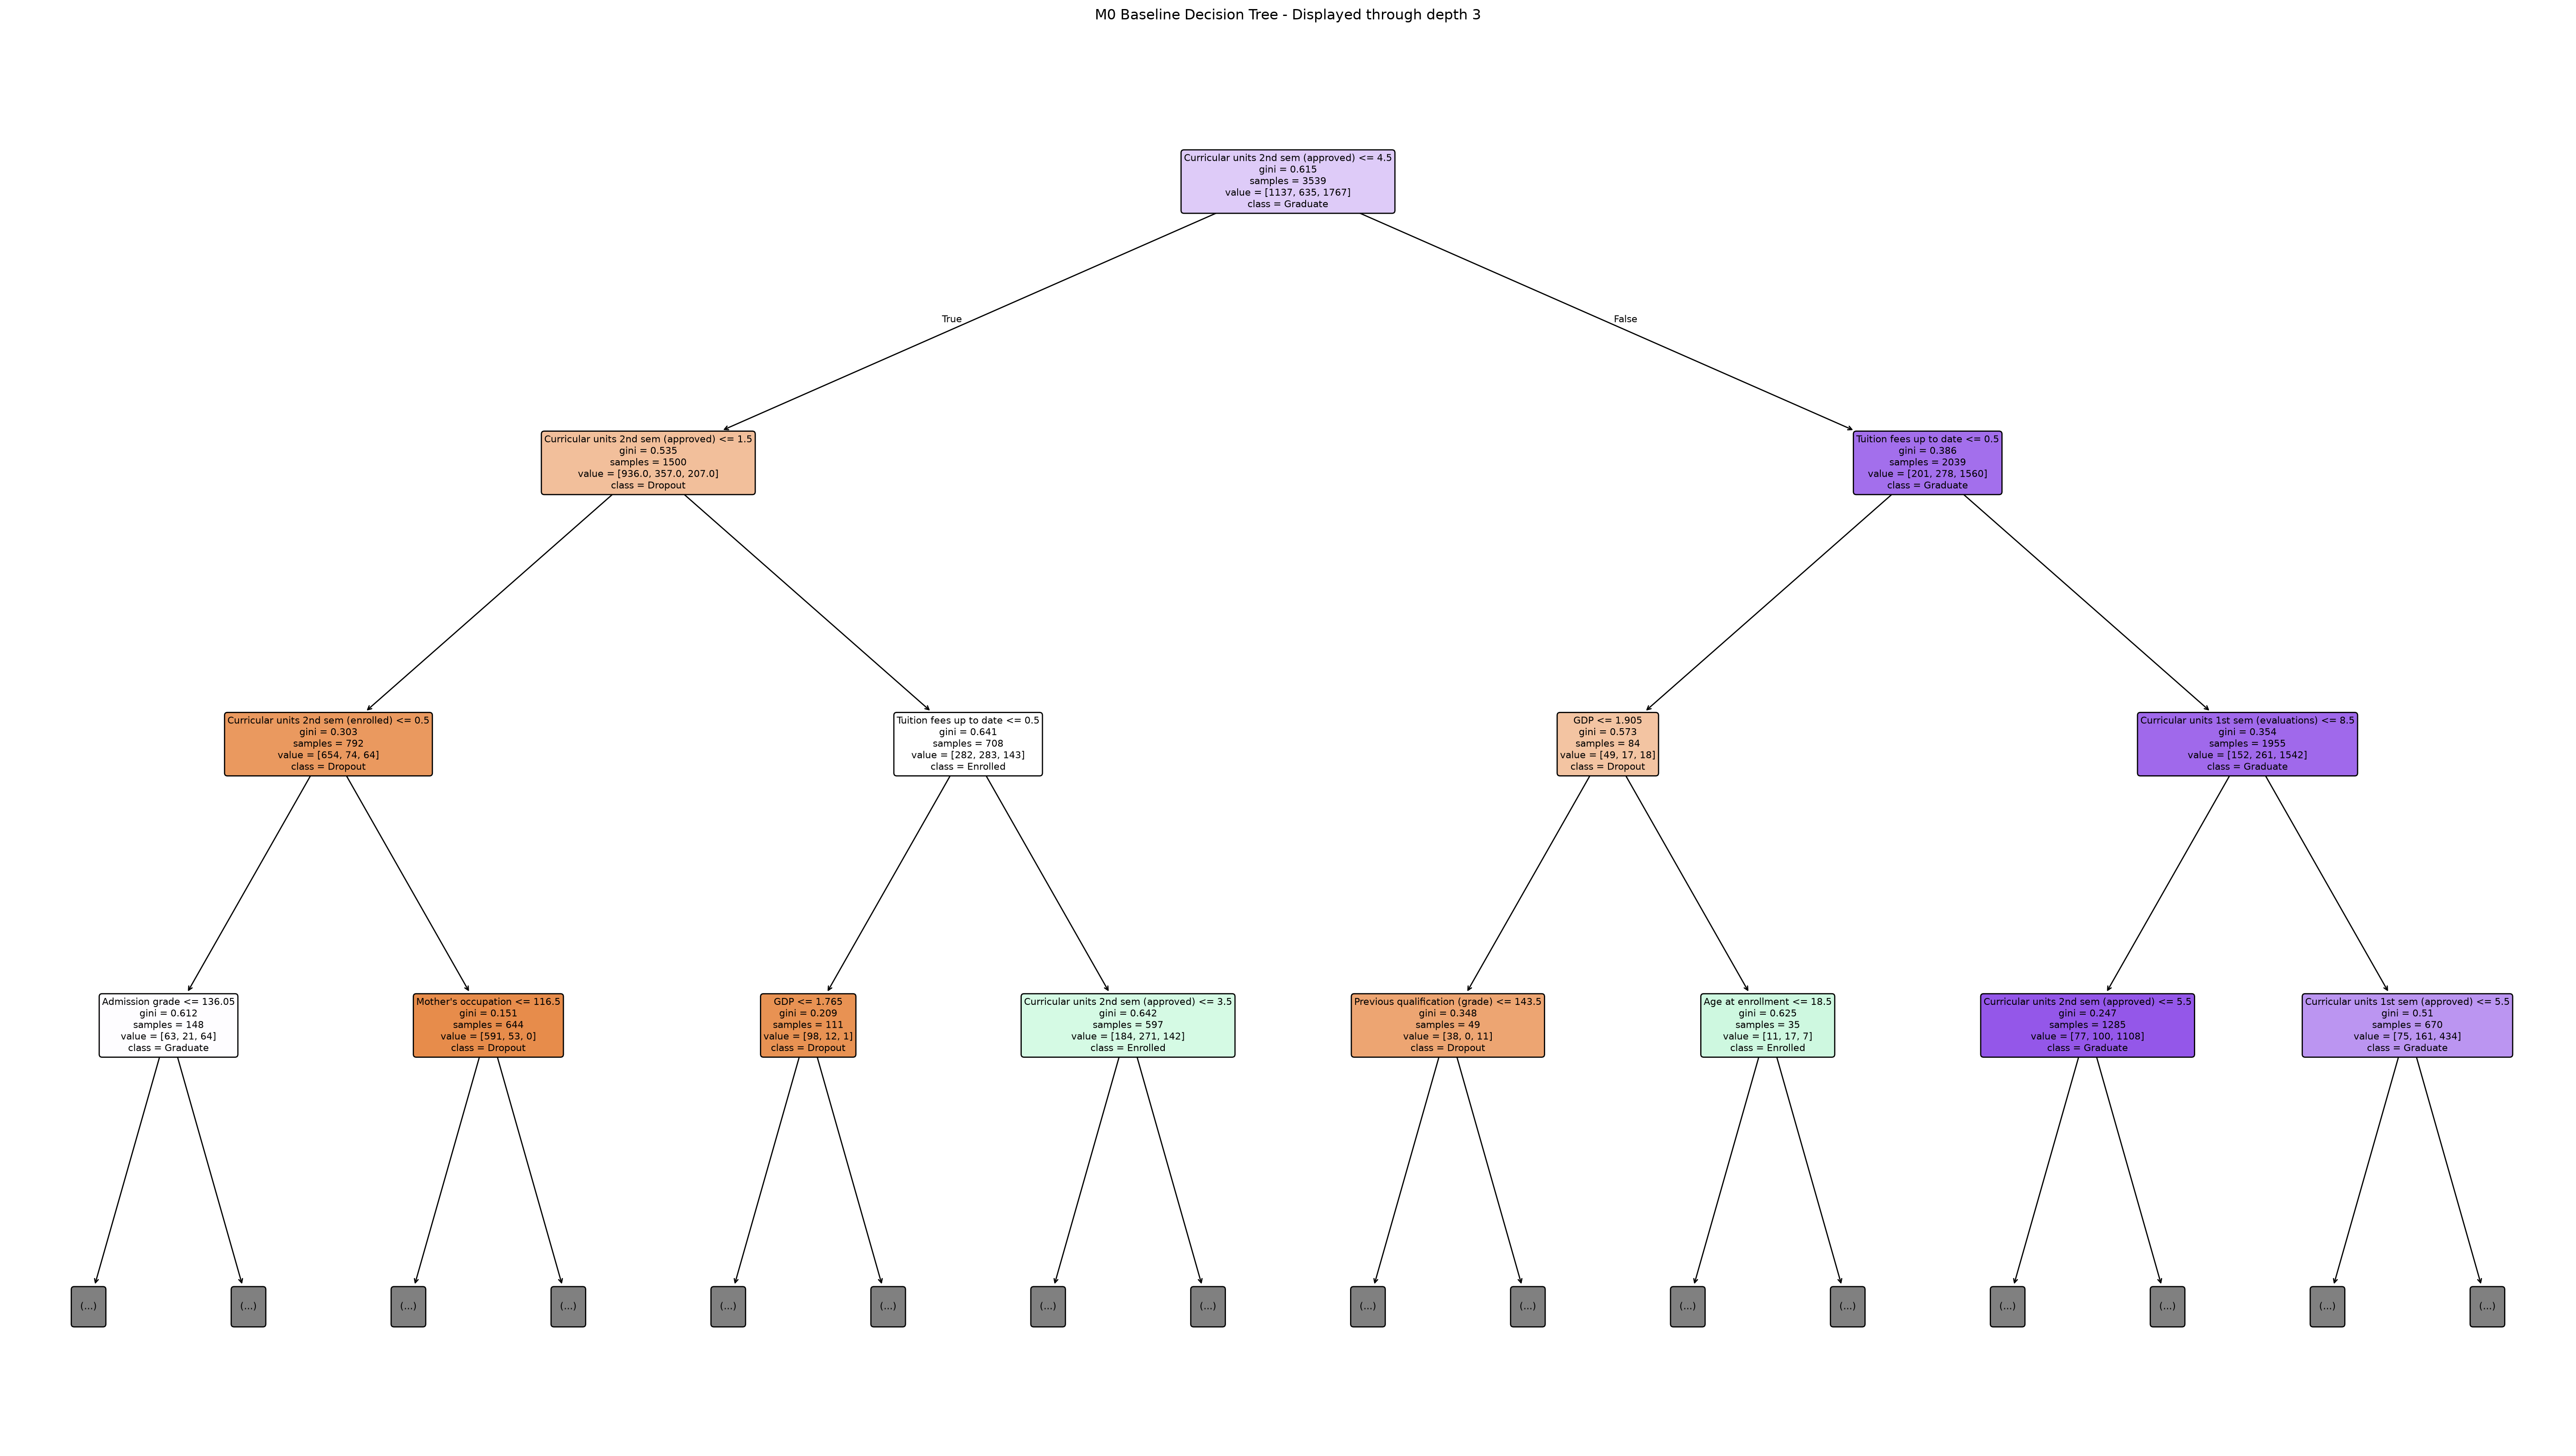
\includegraphics[width=\textwidth]{B_tree_M0_top3.png}
  \caption{\todo{Caption: M0 tree truncated to max\_depth=3 for readability -- describe the root and first splits shown.}}
  \label{fig:d2}
\end{figure}

\subsection{Accuracy and error rate}

\todo{Report train\_acc, test\_acc, error\_rate from \texttt{outputs/results.csv} (M0 row) and \texttt{outputs/classification\_report\_M0.txt}. Include the confusion matrix figure below.}

\begin{figure}[H]
  \centering
  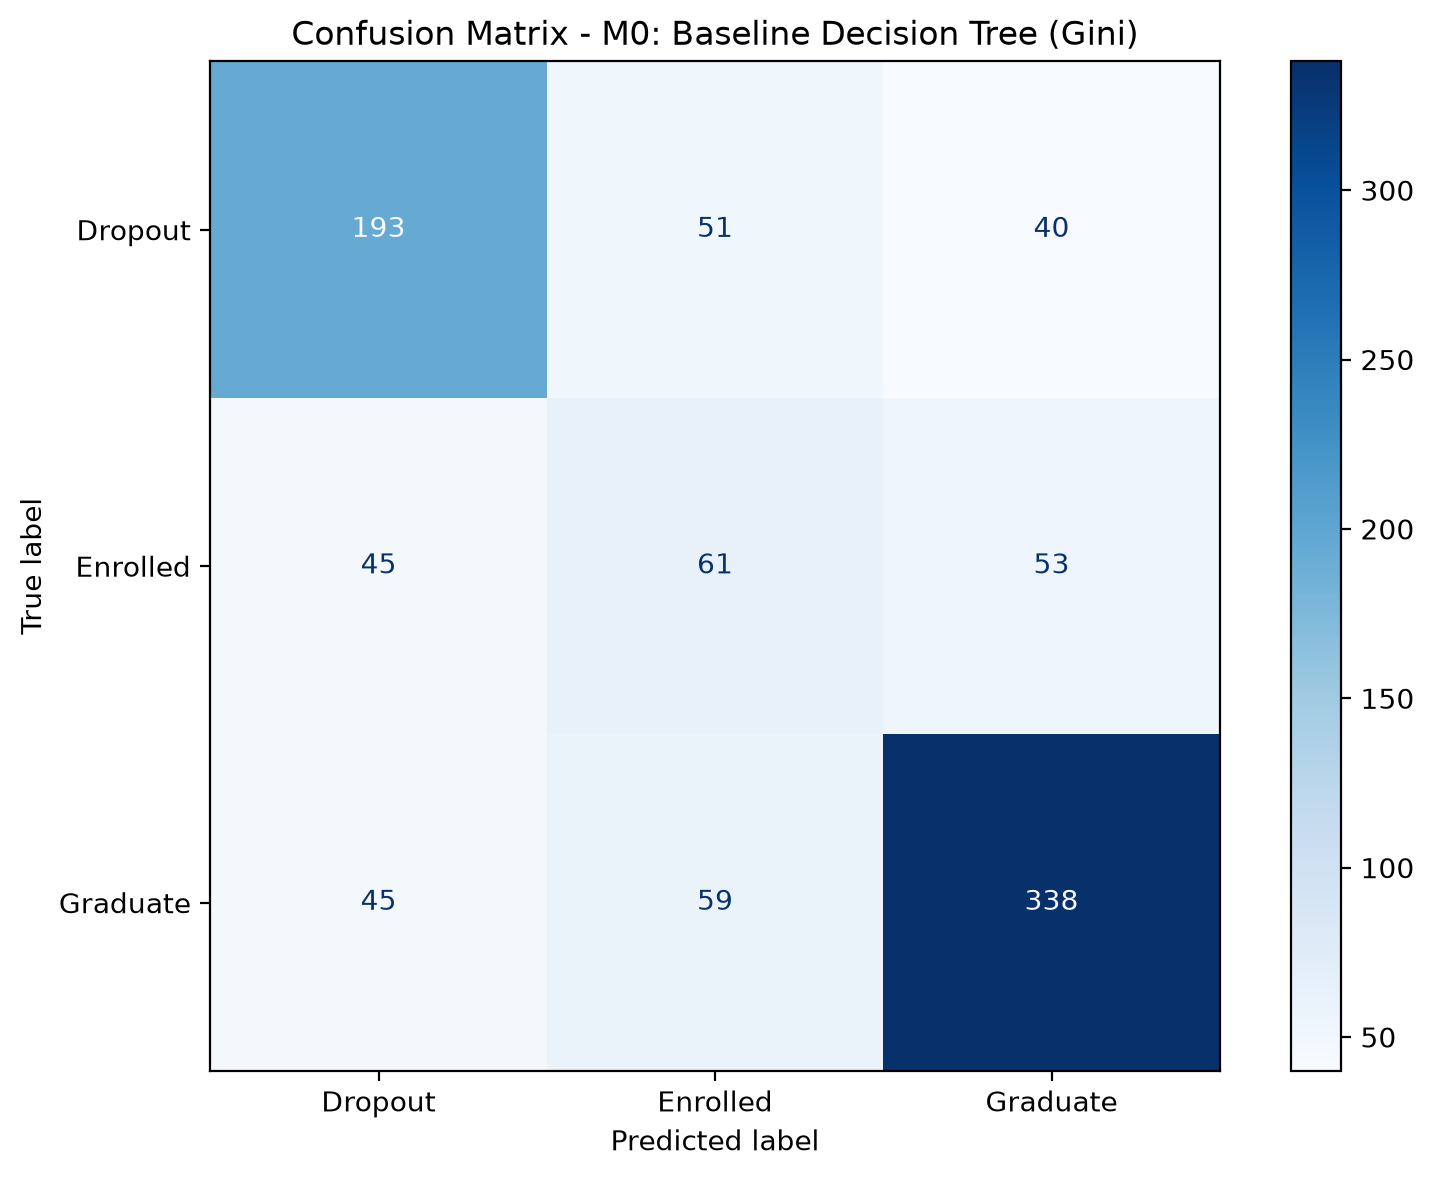
\includegraphics[width=0.7\textwidth]{B_cm_M0.png}
  \caption{\todo{Caption: confusion matrix on the 885-sample held-out test set.}}
  \label{fig:d3}
\end{figure}

\todo{Optional: the Gini-vs-Entropy quick check mentioned in docs/02-DATASET-VA-CONG-VIEC.md C0 note -- one sentence is enough, this is explicitly not one of the 3 official improvements.}

% Owner: Role B. NOT translated yet -- structural skeleton only.
%
% Source material (Vietnamese, already fact-checked -- see progress/A.md
% 2026-08-30 audit: 0 errors out of ~40 checked, including every IF-THEN
% rule condition traced against outputs/rules_M0.txt and every node stat
% re-derived from a fresh retrain): docs/report_draft_d_e.md, bottom part
% (headed "# e. Analysis of the Tree", from "## 1. Root split" onward).
% This is called out in AGENT.md as the single highest-value section of
% the whole report -- do not shorten it when translating.
%
% Brief requires (Section 3.4.e):
%   - Present the generated decision tree.
%   - Comment on its structure and key decision nodes.
%   - Discuss strengths and weaknesses of the baseline tree.
%
% The 5 questions AGENT.md assigns to this section (answer all 5):
%   1. What is the root split, and why did the algorithm pick it?
%   2. What do the first 3 levels of splits mean, in plain language?
%   3. How deep is the tree, how many leaves, any 1-2 sample leaves?
%   4. Train vs test gap -- overfitting evidence?
%   5. 2-3 full IF-THEN rules with sample count and purity.

\section{Analysis of the Tree}
\label{sec:e}

\subsection{Root split}

\todo{Which feature/threshold is the root split, its Gini before/after, and why the algorithm picked it over alternatives.}

\subsection{Root and the next three levels}

\todo{Table or description of the first 3-4 levels: split feature, threshold, sample counts, class distribution, predicted class at each node -- translate the verified node table from the source draft.}

\subsection{Tree complexity}

\todo{Total node/leaf count, \% of leaves with 1-2 samples, average leaf depth -- and what that says about overfitting risk.}

\subsection{Overfitting evidence}

\todo{Train vs.\ test accuracy gap (generalization gap), and whether it falls in the expected 0.65--0.72 test-accuracy band from AGENT.md (a red flag if not).}

\subsection{Representative IF-THEN rules}

\todo{Translate the 3 rules from the source draft verbatim (Dropout, Graduate, Enrolled), each with the full condition chain, leaf sample count $n$, and purity. Do not paraphrase the conditions loosely -- copy the exact feature/threshold values, they were independently re-verified against \texttt{outputs/rules\_M0.txt}.}

\begin{quote}
\emph{Example rule format (replace with the real translated rules):} \\
IF \texttt{Curricular units 2nd sem (approved)} $\le$ 1.5 AND \ldots \\
THEN \textbf{Dropout} ($n = 189$, purity 100\%).
\end{quote}

\subsection{Strengths and weaknesses of the baseline tree}

\todo{Summarize: strengths (readable top splits, handles nonlinearity, no scaling needed) vs.\ weaknesses (hard to present as a whole, unstable predictions, especially weak on Enrolled, uses semester-outcome features so not usable for early warning).}

\begin{quote}
\todo{Ethical/limitations note (see source draft's own closing section): sensitive features (gender, \texttt{Nacionality}, marital status, parents' occupation/education) appear in some rule conditions -- these must be flagged as correlational, not causal, and not used as grounds for discrimination.}
\end{quote}


\section{f. Improvement Methods}
\label{sec:f}
% The brief requires 2-3 improvement methods, each presented separately
% with: description, modified tree/model setting, accuracy + error rate,
% and an explanation of why it does (or does not) improve the result.
% This project implements exactly 3: pruning (C), class imbalance (D),
% feature selection for early warning (E). Each is its own \subsection
% in its own file below -- do not merge them into one file.
% Owner: Role C. NOT translated yet -- structural skeleton only.
%
% Source material (Vietnamese, already fact-checked -- progress/A.md
% 2026-08-30 audit: 0 errors out of ~40 checked, including the full 16-cell
% grid search table and independent re-run of cost_complexity_pruning_path):
% docs/report_draft_f1_pruning.md.
%
% Brief requires, for EACH improvement method (Section 3.4.f):
%   - Description of the method
%   - Modified tree or model setting
%   - Accuracy and error rate
%   - Explanation of why the method improves (or does not improve) the result
%
% Figures already committed and ready to reference (do not rename):
%   figures/C_ccp_alpha_curve.png  -- pruning path + CV-accuracy-vs-alpha
%   figures/C_tree_M1.png          -- pruned tree (depth 5, 17 leaves)
%   figures/C_cm_M1.png            -- confusion matrix

\subsection{f.1 Improvement Method 1: Cost-Complexity Pruning}
\label{sec:f1}

\subsubsection{Method description}

\todo{Describe cost-complexity pruning, candidate alpha generation, and alpha selection by cross-validation on training data only. Include the required depth grid $\{5,8,10,15\}$ and minimum-leaf-size grid $\{1,5,10,20\}$. State explicitly that test accuracy never selected hyperparameters.}

\subsubsection{Modified tree / model setting}

\todo{Report the selected alpha, depth cap, minimum leaf size, random seed, and the cross-validation accuracy that selected the configuration.}

\begin{figure}[H]
  \centering
  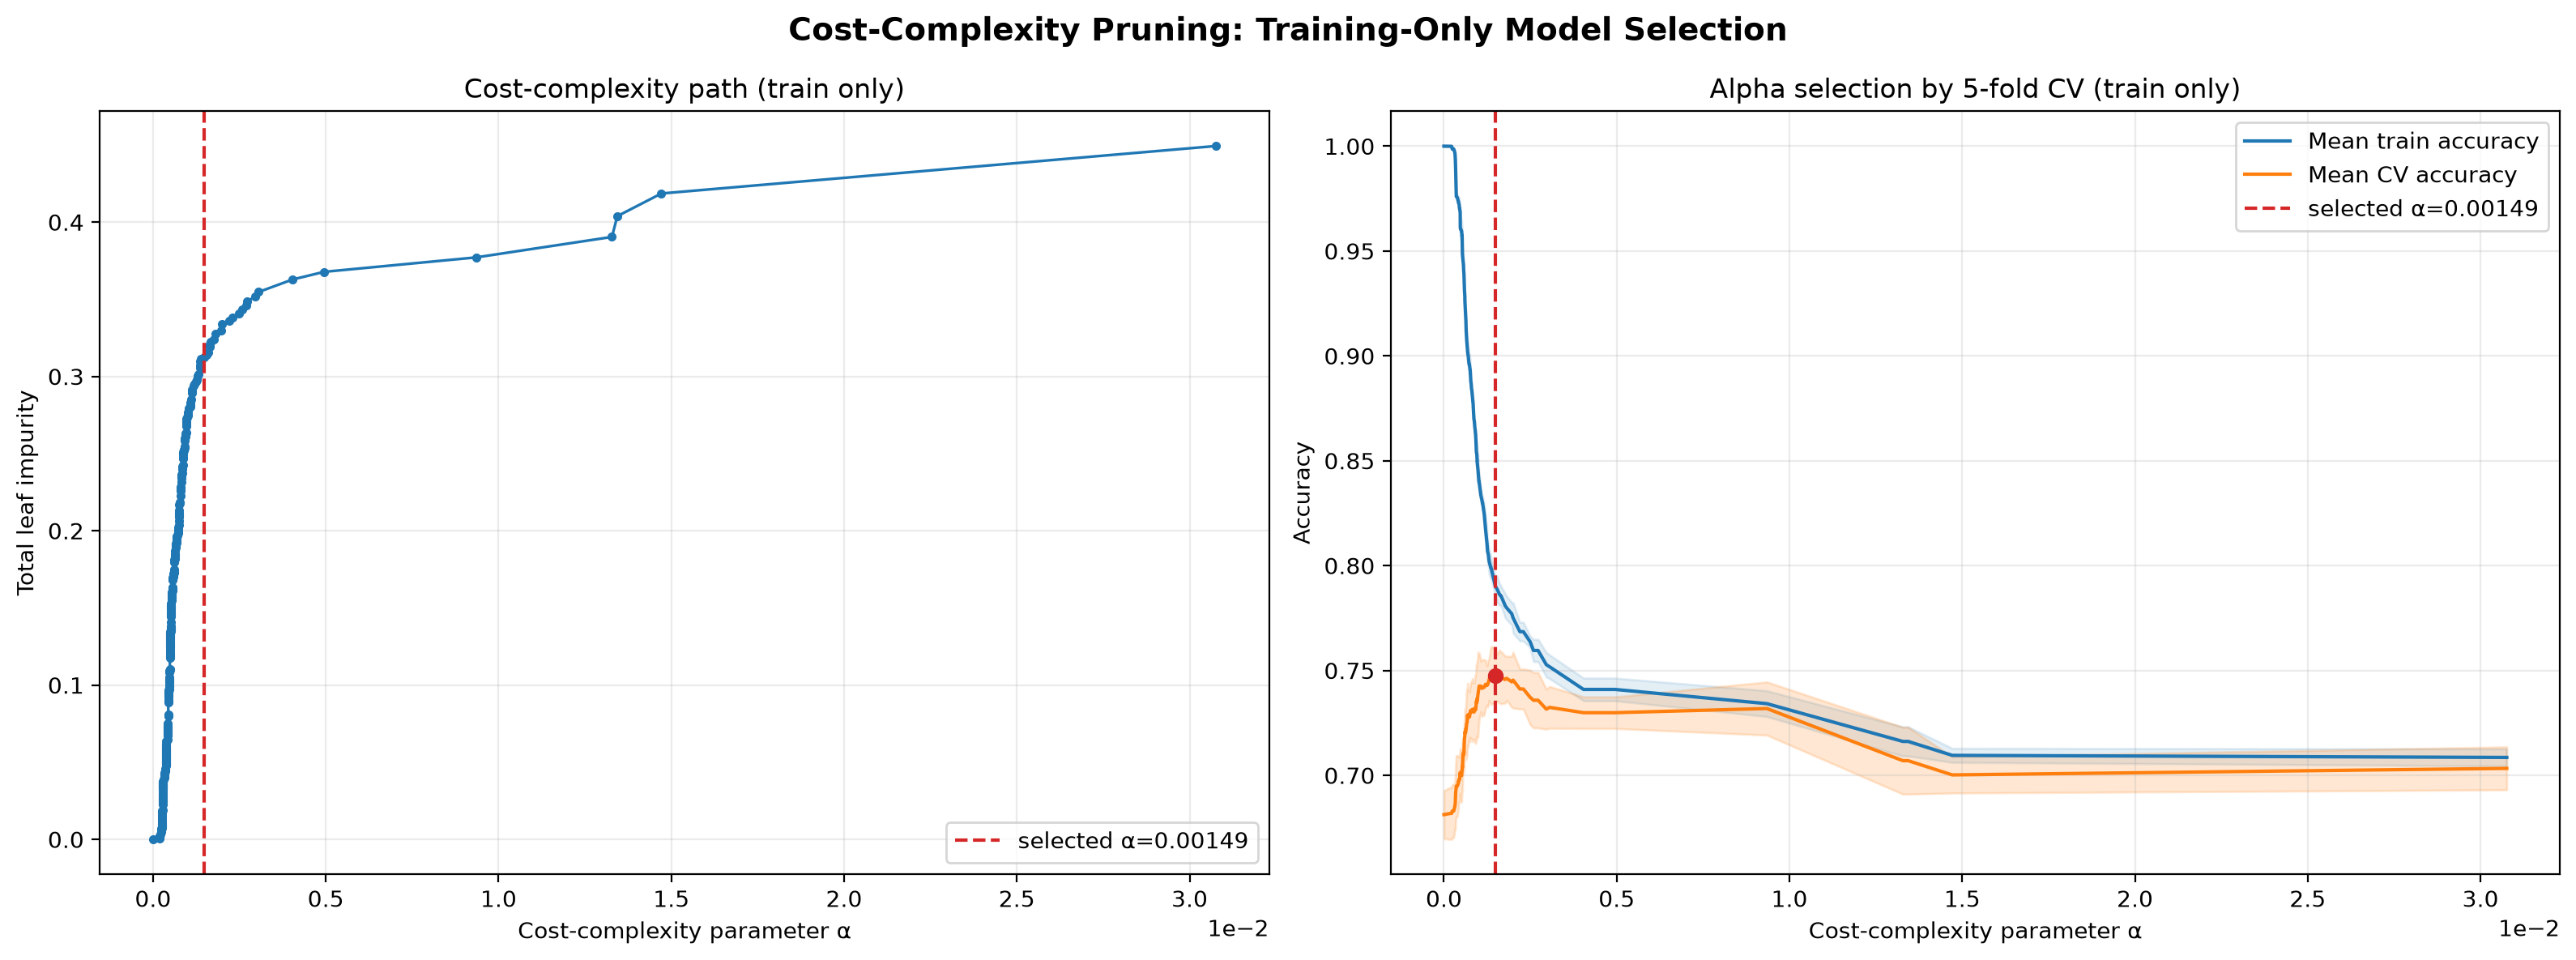
\includegraphics[width=0.9\textwidth]{C_ccp_alpha_curve.png}
  \caption{\todo{Caption: left panel = leaf impurity vs.\ alpha; right panel = train/CV accuracy with the selected alpha marked. No test curve, by design.}}
  \label{fig:f1a}
\end{figure}

\begin{figure}[H]
  \centering
  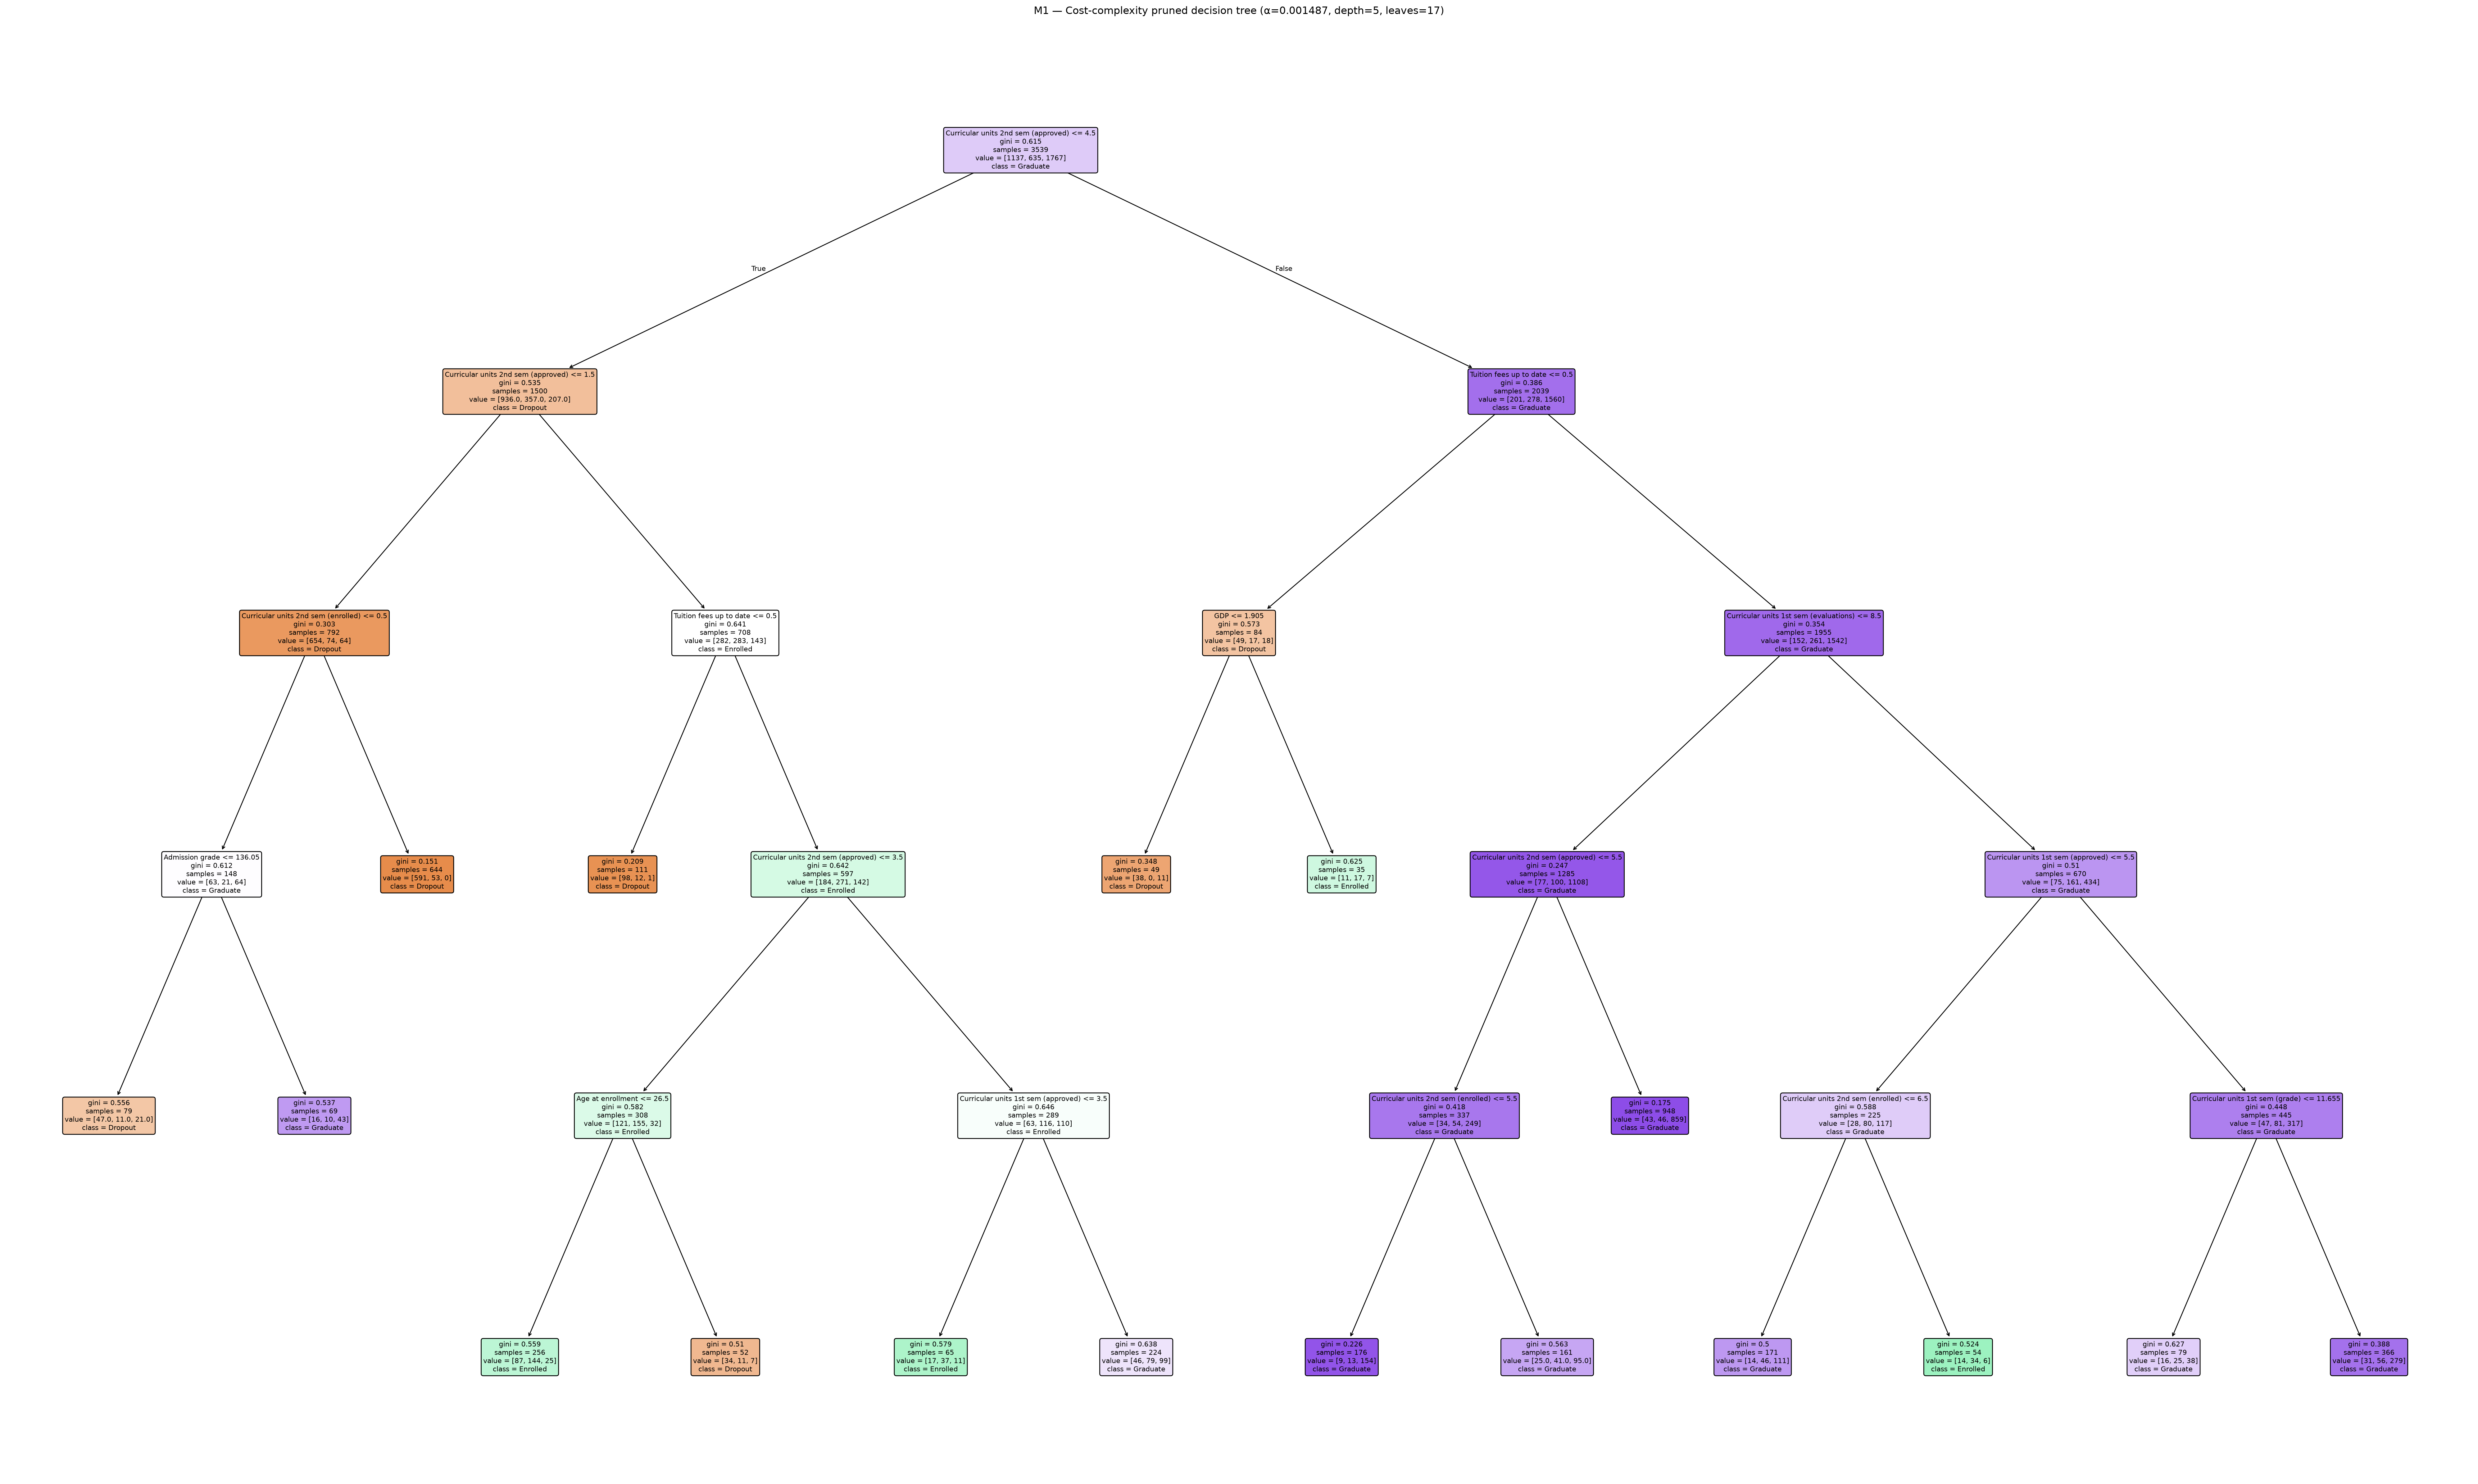
\includegraphics[width=0.75\textwidth]{C_tree_M1.png}
  \caption{\todo{Caption: the pruned M1 tree (depth 5, 17 leaves) -- small enough to read and use for rule extraction, unlike M0.}}
  \label{fig:f1b}
\end{figure}

\subsubsection{Accuracy and error rate}

\todo{Report M1's test\_acc / error\_rate from \texttt{outputs/results.csv} and compare against M0 (test\_acc 0.6689, error\_rate 0.3311). Include the confusion matrix.}

\begin{figure}[H]
  \centering
  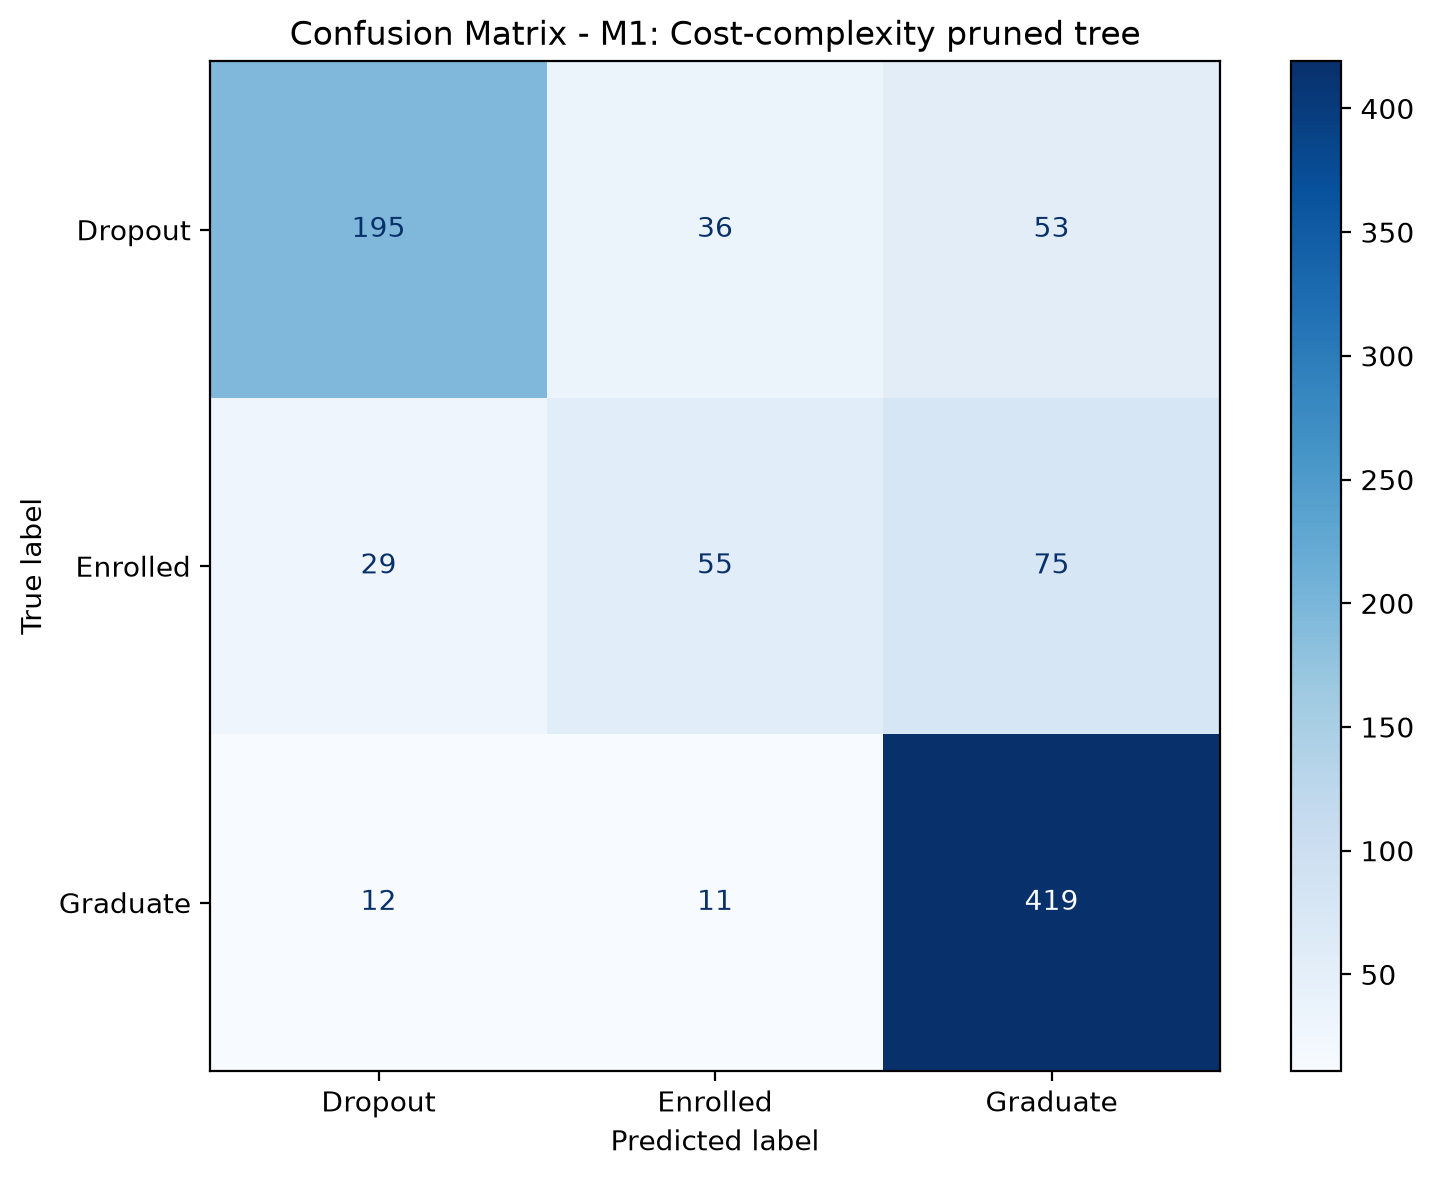
\includegraphics[width=0.6\textwidth]{C_cm_M1.png}
  \caption{\todo{Caption: confusion matrix on the same 885-sample held-out test set as M0.}}
  \label{fig:f1c}
\end{figure}

\subsubsection{Why this improves the result}

\todo{Explain why accuracy went up while the tree got dramatically smaller (fewer leaves = less noise memorized, not less signal). Also discuss the one trade-off: which per-class recall got worse, and why (accuracy was the pre-declared CV selection criterion, so the config was free to favor the majority class if that raised the total correct count).}

% Final section; metrics, class reports, resampling counts, and categorical
% audits were checked against the canonical M2a/M2b experiment artifacts.

\subsection{Improvement Method 2: Class Imbalance}
\label{sec:f2}

\subsubsection{Motivation}
\label{sec:f2-motivation}

The target variable of the dataset is unevenly distributed across the three outcome
classes: \textit{Graduate} is the majority class, \textit{Dropout} is the second
largest, and \textit{Enrolled} is a clear minority. On the shared held-out test set
of 885 students, the baseline model M0 correctly classifies 338 of 442
\textit{Graduate} students and 193 of 284 \textit{Dropout} students, but only 61 of
159 \textit{Enrolled} students. Consequently, although M0 achieves an overall test
accuracy of $0.668927$, its recall on the \textit{Enrolled} class is only
$0.383648$. This is a material limitation whenever the intended application requires
identifying students who are not on track to graduate on time, rather than merely
maximizing the number of correct predictions on the majority class.

Improvement Method 2 (M2) evaluates two complementary ways of increasing a decision
tree's sensitivity to minority classes: reweighting the training objective
(\textbf{M2a}) and synthetically rebalancing the training distribution
(\textbf{M2b}). Both configurations reuse the project's single stratified
train/test split
(3{,}539 training rows and 885 held-out test rows, 90 features after one-hot
encoding, \texttt{random\_state=42}); no feature scaling and no independent
re-splitting are performed in the notebook, consistent with the project-wide data
contract.

\subsubsection{Method description}
\label{sec:f2-method}

\textbf{M2a - class weighting.} M2a trains a single
\texttt{DecisionTreeClassifier} with \texttt{class\_weight=}\allowbreak\texttt{`balanced'} and
\texttt{random\_state=42}, fit directly on the original (non-resampled) training
data:
\begin{quote}
\texttt{DecisionTreeClassifier(class\_weight='balanced', random\_state=42)}
\end{quote}
Under this setting, scikit-learn scales each class's contribution to the impurity
criterion inversely to its frequency in the training data. No synthetic samples are
created; the sample size and the feature space are identical to those used by M0.

\textbf{M2b - Synthetic Minority Over-sampling Technique (SMOTE).} M2b applies
SMOTE \citep{chawla2002smote,imblearn_smote_api} to the training split only, after
the shared split has already been produced, and fits an otherwise unmodified
decision tree on the resampled data:
\begin{quote}
\texttt{X\_train\_smote, y\_train\_smote = SMOTE(} \\
\indent \texttt{sampling\_strategy="auto", random\_state=42, k\_neighbors=5} \\
\texttt{).fit\_resample(X\_train, y\_train)} \\
\texttt{DecisionTreeClassifier(random\_state=42)} \\
\indent \texttt{.fit(X\_train\_smote, y\_train\_smote)}
\end{quote}
All three SMOTE hyperparameters are declared explicitly rather than left to their
library defaults, so that the resulting artifact does not silently change if a
future \texttt{imbalanced-learn} release alters its default behavior
\citep{imblearn_oversampling_guide}. Before resampling, the training split contains
1{,}137 \textit{Dropout}, 635 \textit{Enrolled}, and 1{,}767 \textit{Graduate}
samples. After resampling, every class contains exactly 1{,}767 samples, for a total
of 5{,}301 training rows (1{,}762 synthetic rows).

\textbf{Leakage safeguard.} SMOTE is applied strictly \emph{after} the train/test
split and is fit exclusively on \texttt{X\_train}/\texttt{y\_train}. Exposing
the test set to resampling would cause data leakage, so the experiment also computes a
value-, index-, shape-, column-order-, and dtype-aware fingerprint of
\texttt{X\_train}, \texttt{X\_test}, \texttt{y\_train}, and \texttt{y\_test}
immediately before calling \texttt{SMOTE.fit\_resample()}, and asserts that all four
fingerprints are bit-for-bit unchanged immediately afterwards. The evaluation
itself is likewise performed only on the original, untouched \texttt{X\_test}/
\texttt{y\_test}; the resampled training data is used exclusively to fit the model,
never to compute any reported metric.

\subsubsection{Modified tree / model setting}
\label{sec:f2-figures}

\begin{figure}[H]
  \centering
  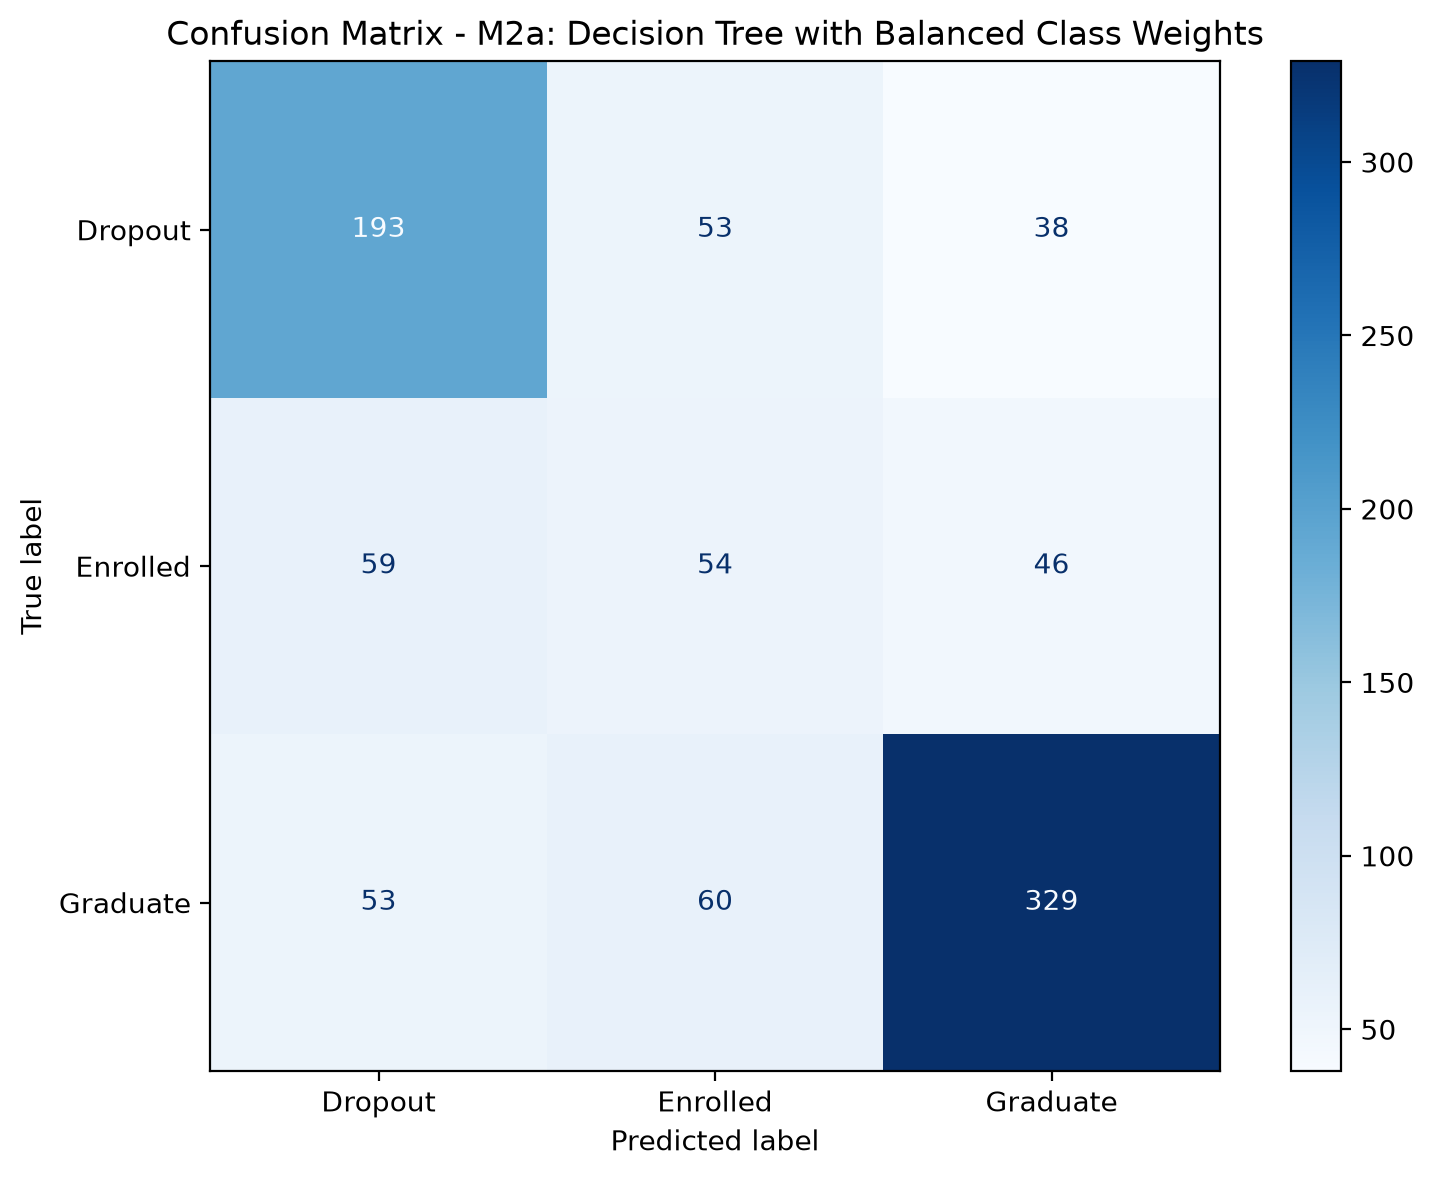
\includegraphics[width=0.75\textwidth]{D_cm_M2a.png}
  \caption{Confusion matrix of M2a (balanced class weights) on the 885-sample
  held-out test set.}
  \label{fig:cm-m2a}
\end{figure}

\begin{figure}[H]
  \centering
  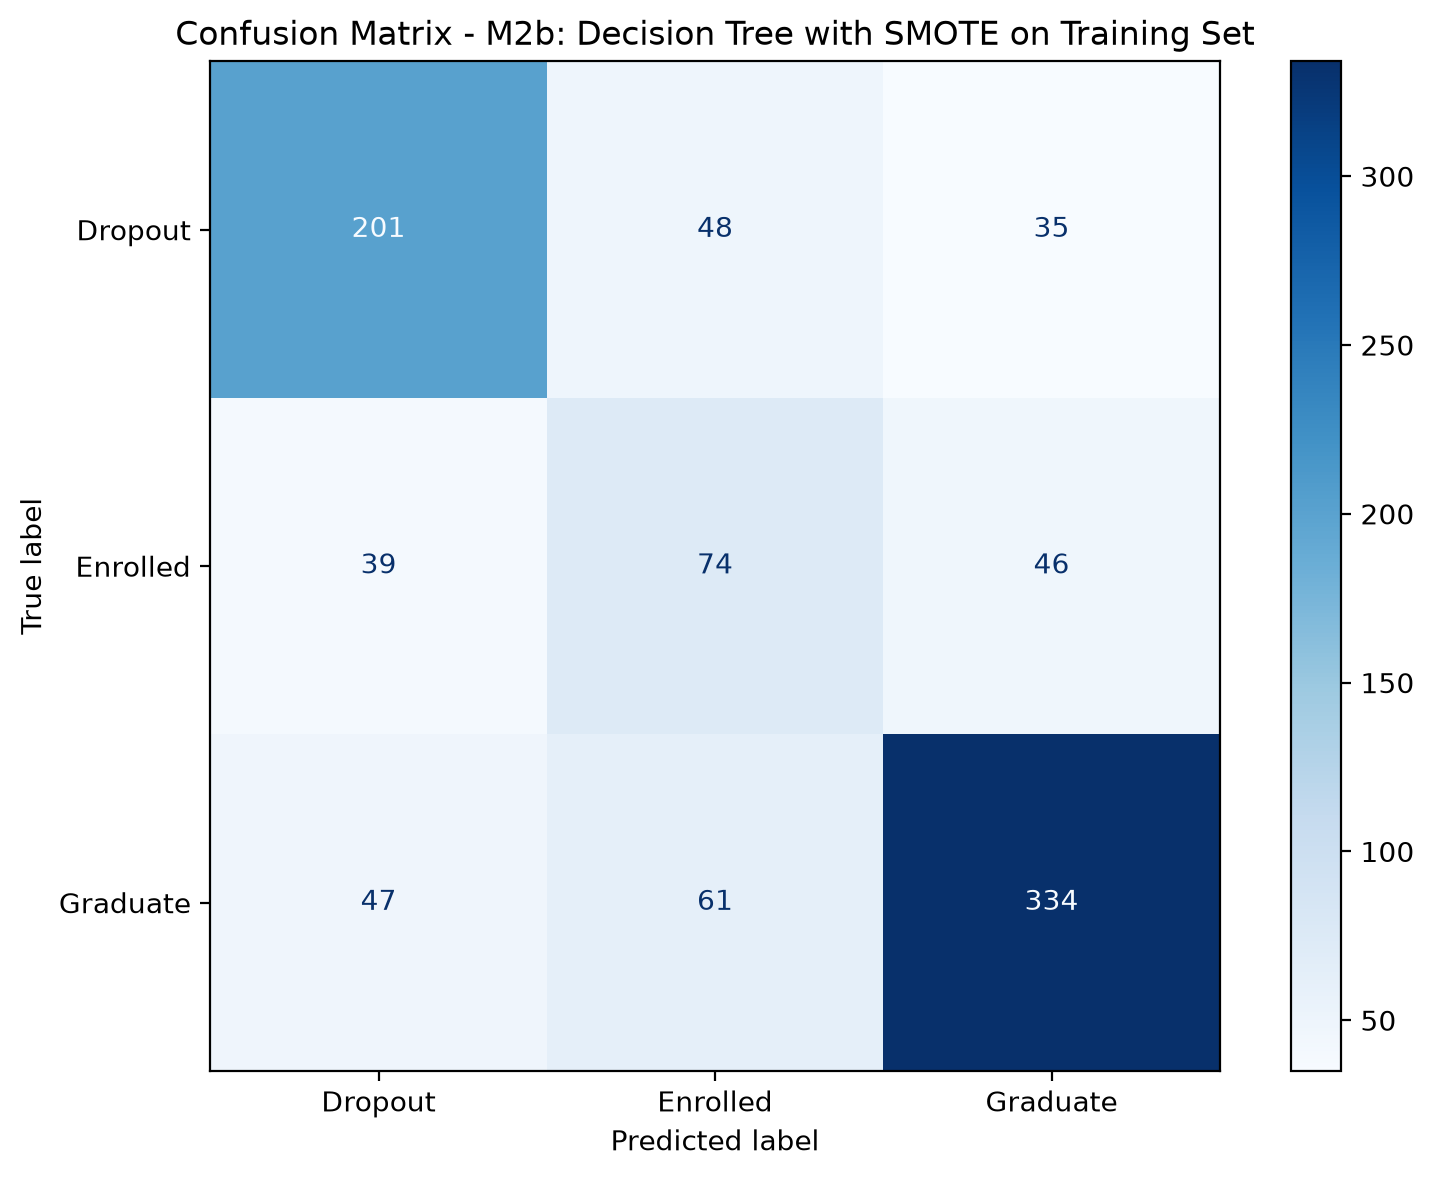
\includegraphics[width=0.75\textwidth]{D_cm_M2b.png}
  \caption{Confusion matrix of M2b on the 885-sample held-out test set.}
  \label{fig:cm-m2b}
\end{figure}

M2b correctly classifies 201 Dropout and 74 Enrolled students, exceeding
both M0 (193 and 61) and M2a (193 and 54). It correctly classifies 334
Graduate students, more than M2a (329) but fewer than M0 (338).

\begin{figure}[H]
  \centering
  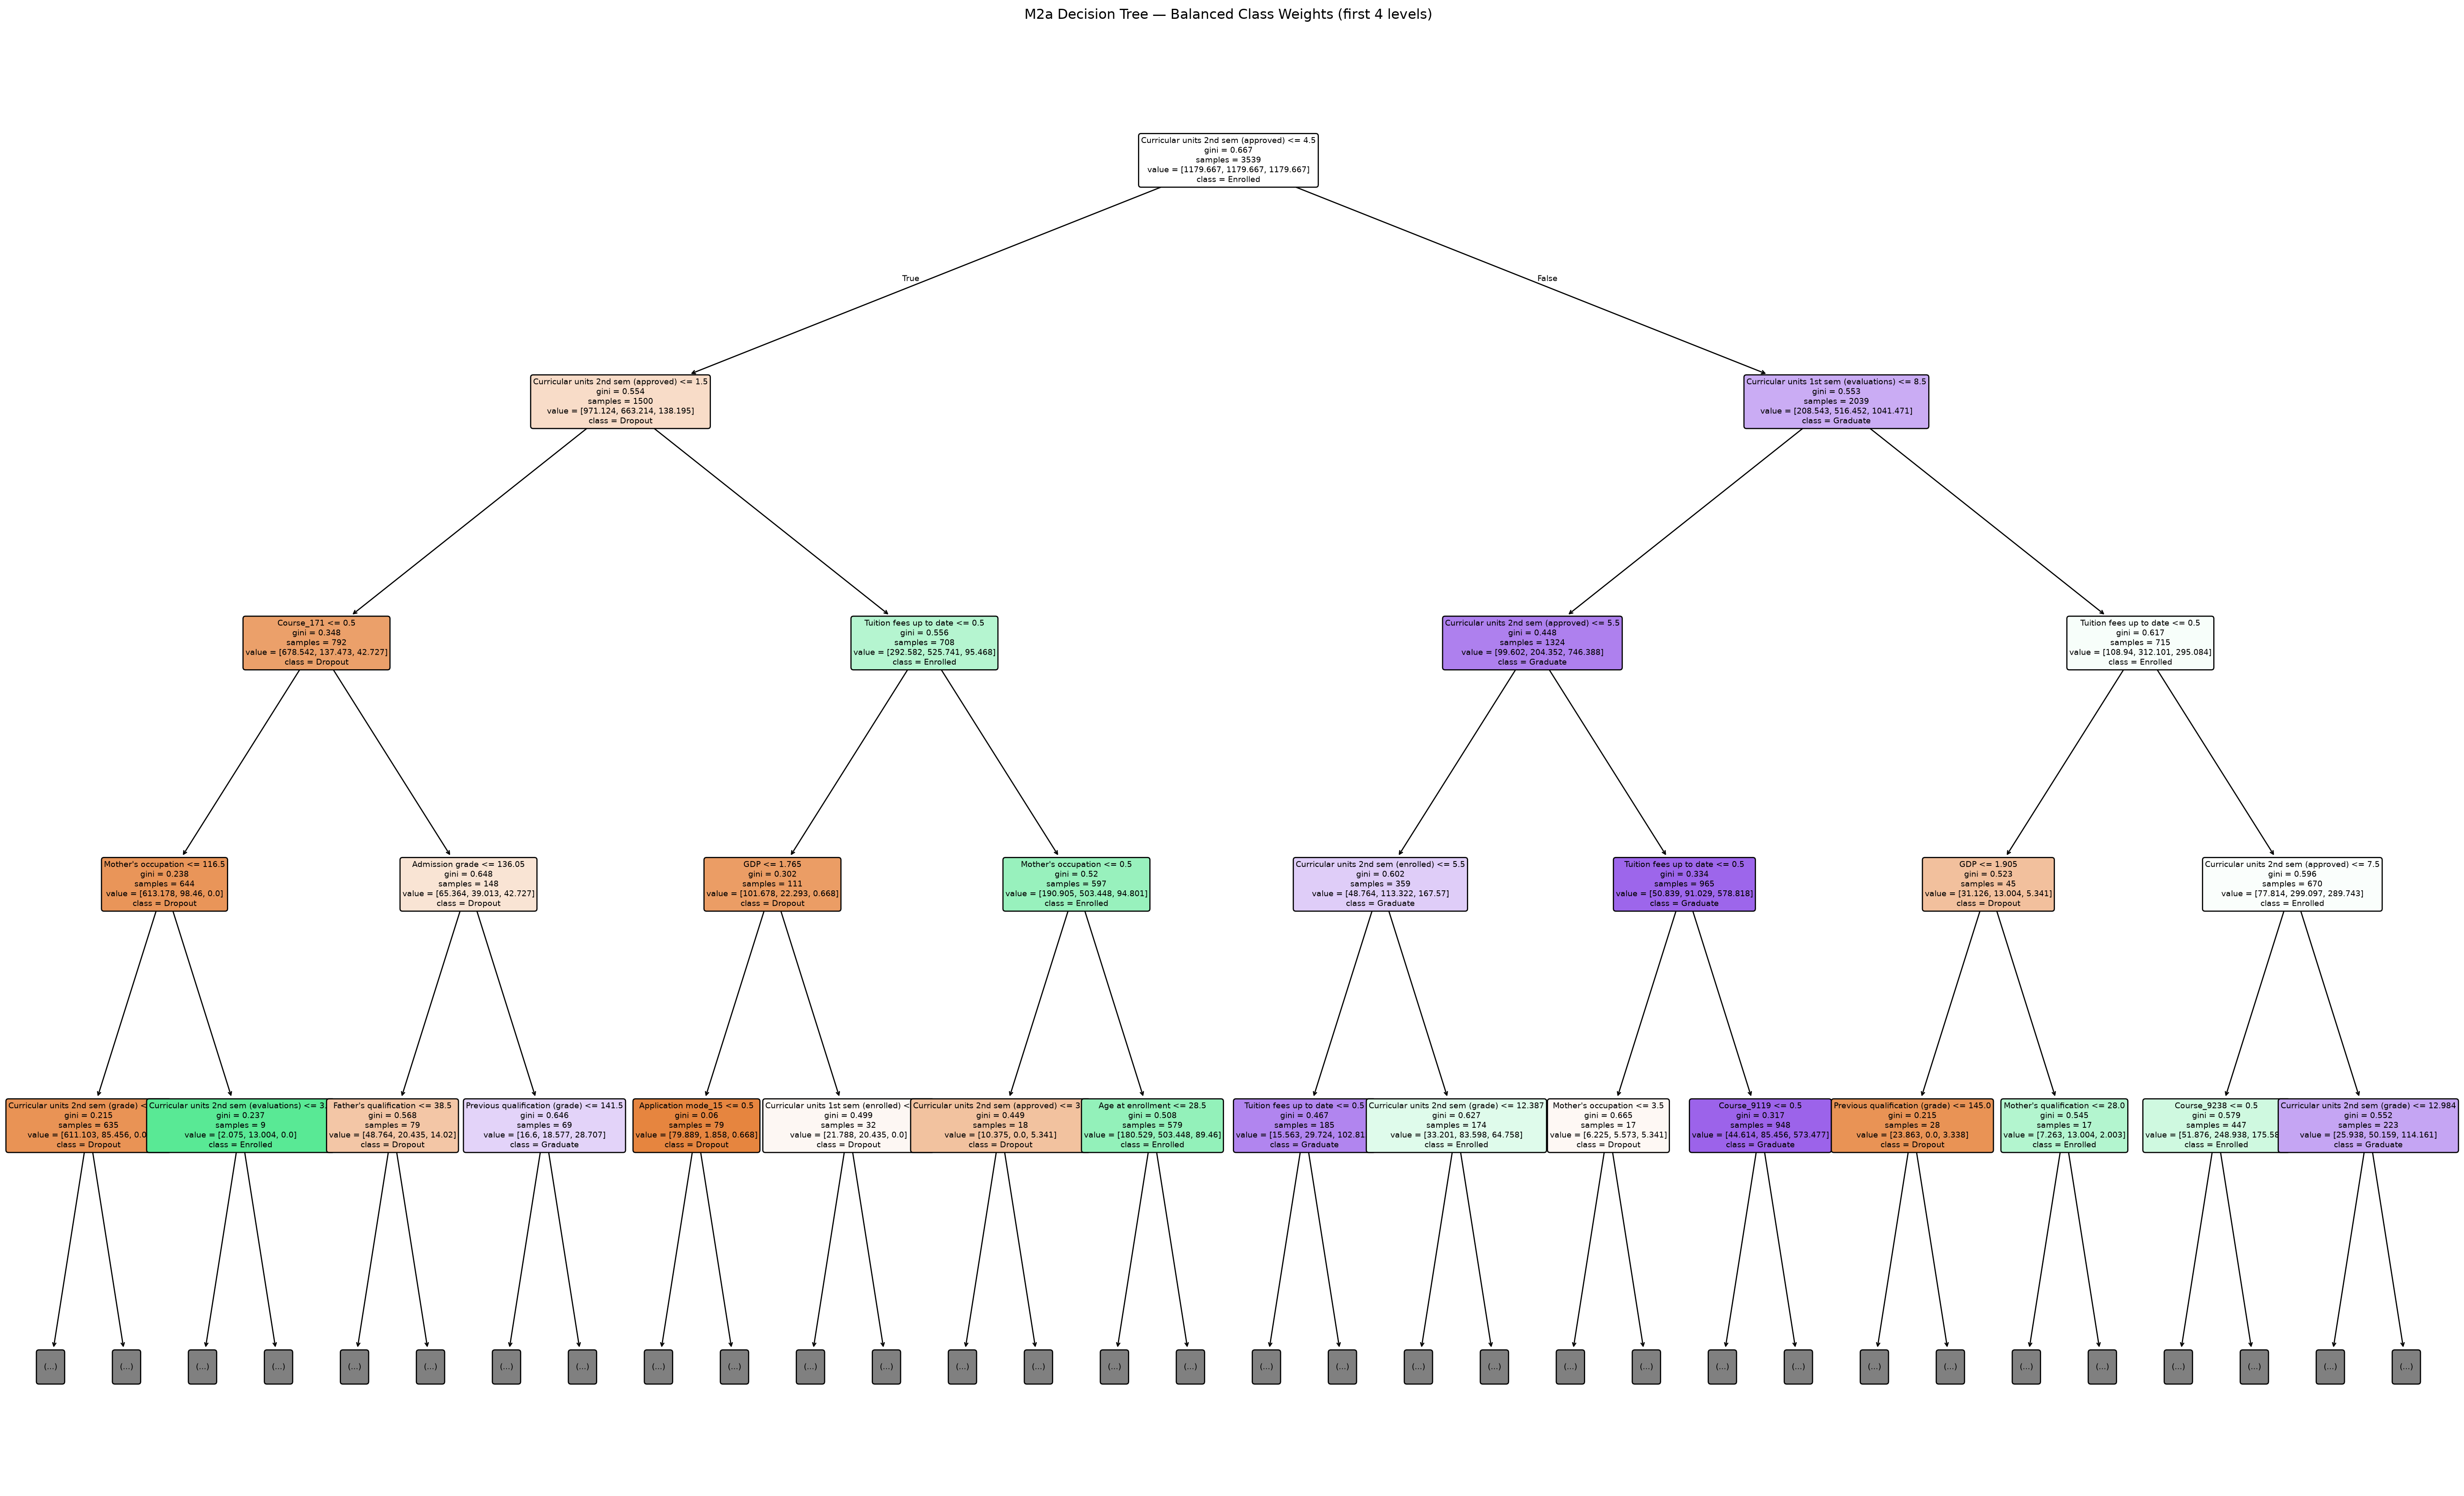
\includegraphics[width=1\textwidth]{D_tree_M2a.png}
  \caption{M2a decision tree, truncated to the first four levels for
  legibility. The fitted tree has a true depth of 28 and 696 leaves.}
  \label{fig:tree-m2a}
\end{figure}

\begin{figure}[H]
  \centering
  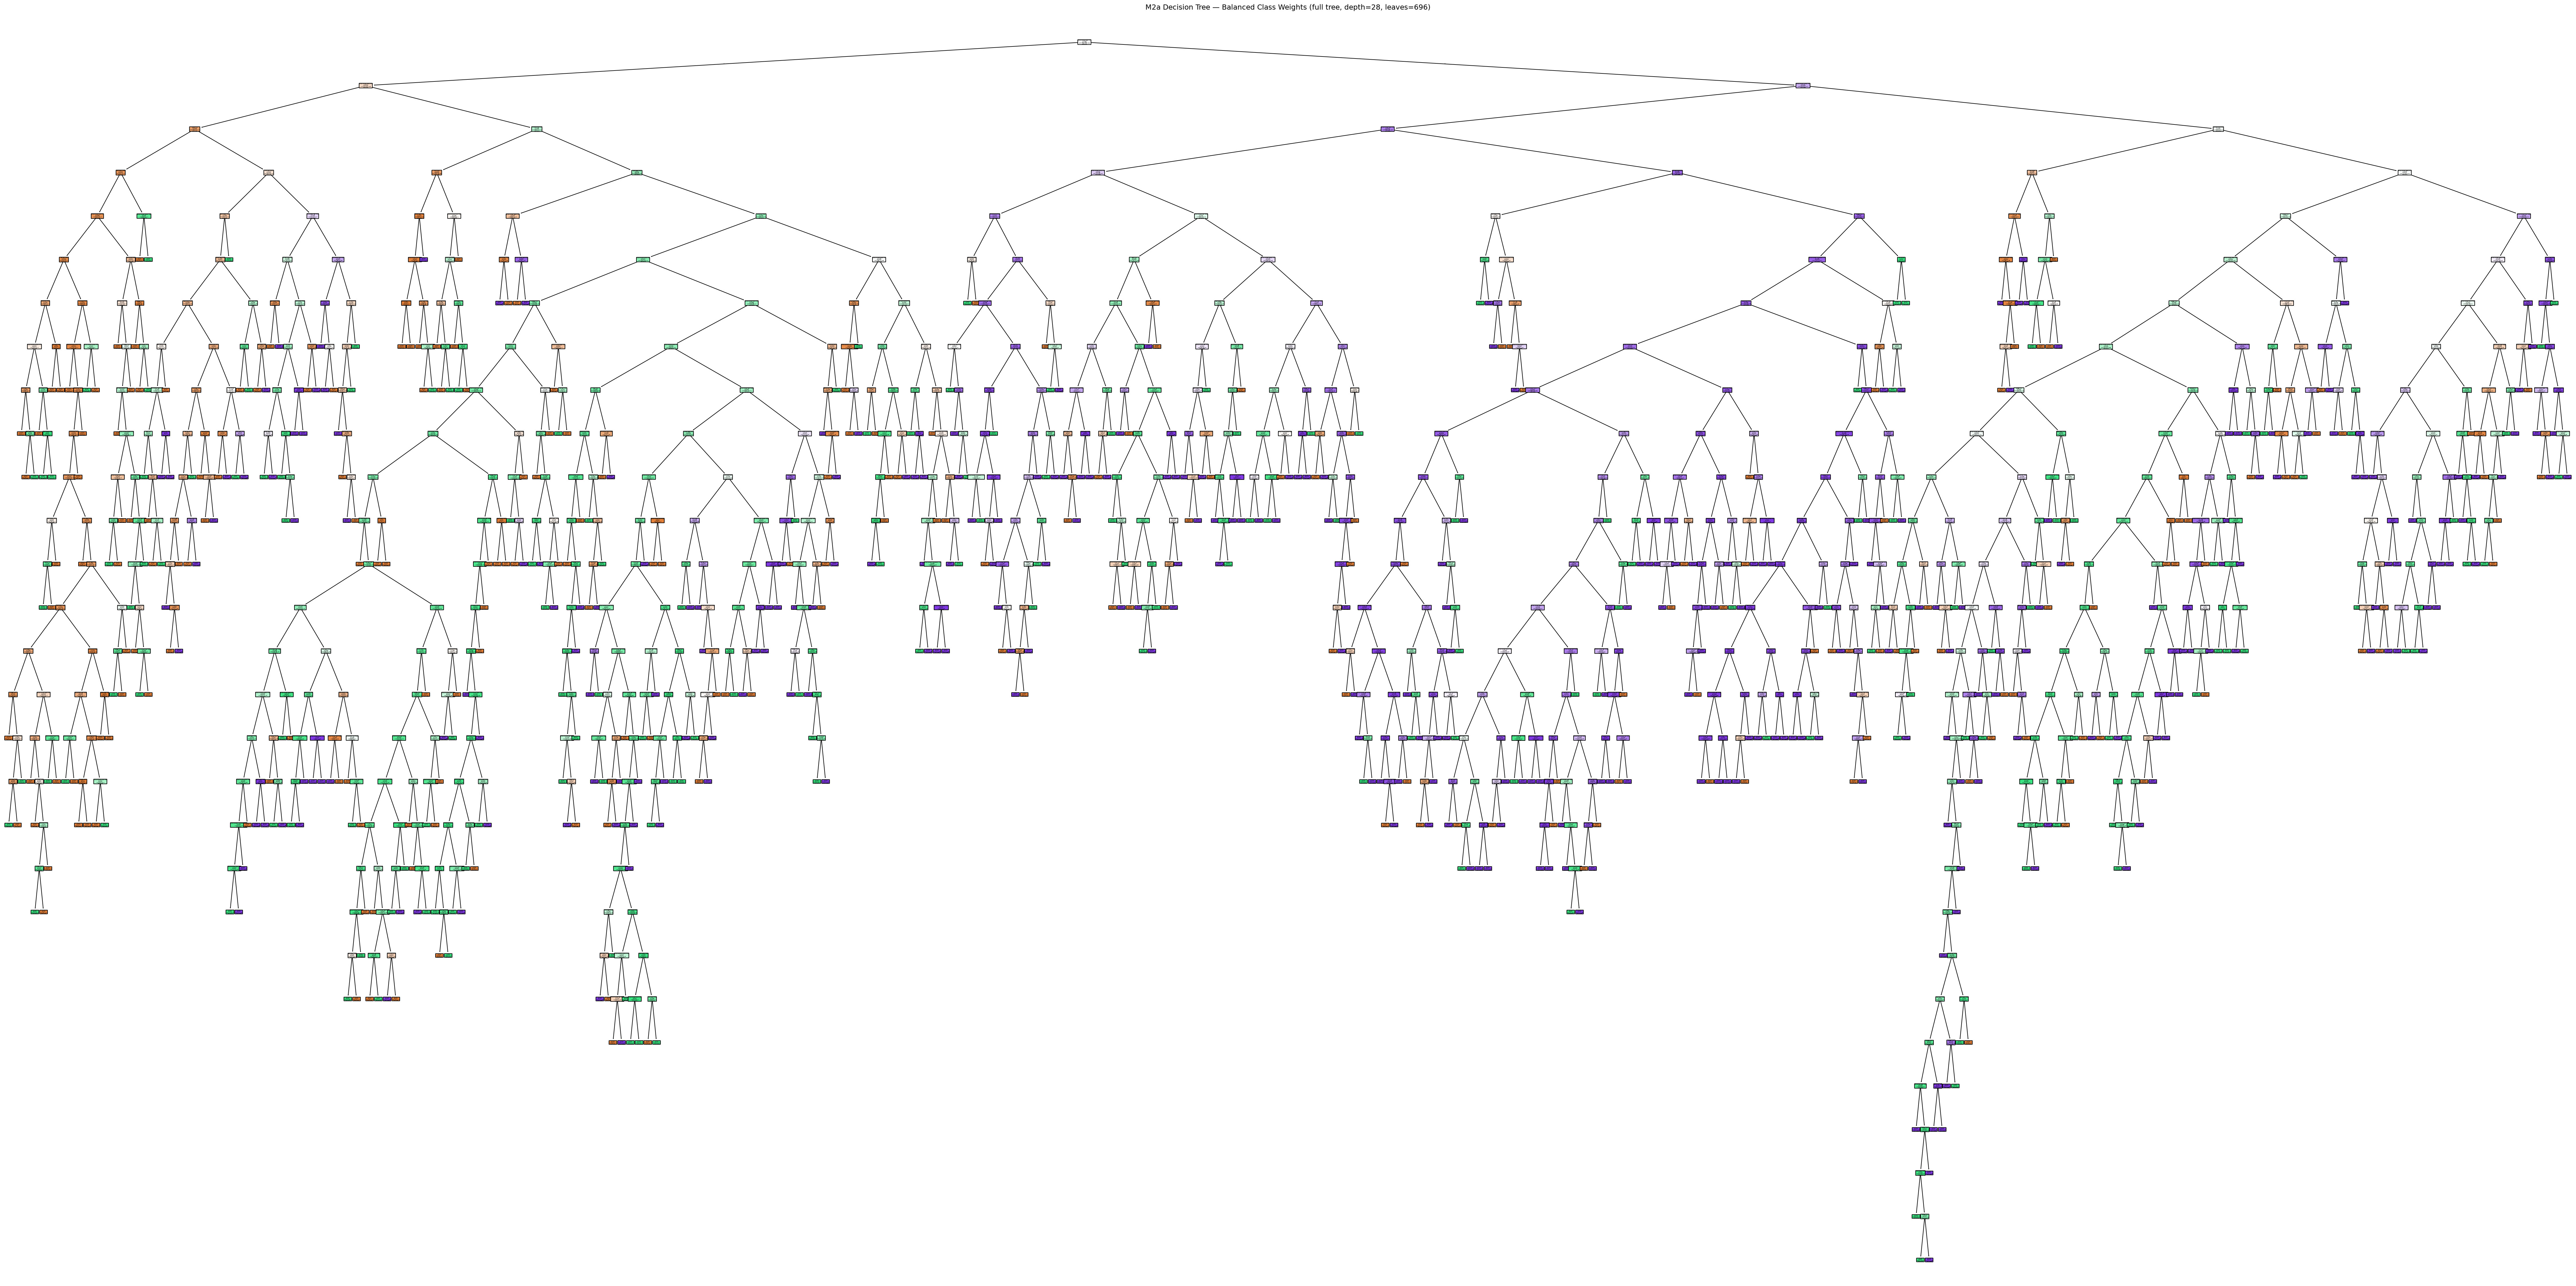
\includegraphics[width=1\textwidth]{D_tree_M2a_full.png}
  \caption{Full M2a decision tree (depth 28, 696 leaves).}
  \label{fig:tree-m2a-full}
\end{figure}

The full M2a view is not intended for node-by-node reading. Reweighting the
classes changes which splits the tree prioritizes, but the fitted tree remains
close to M0 in structural size (depth 27 and 634 leaves for M0).

\begin{figure}[H]
  \centering
  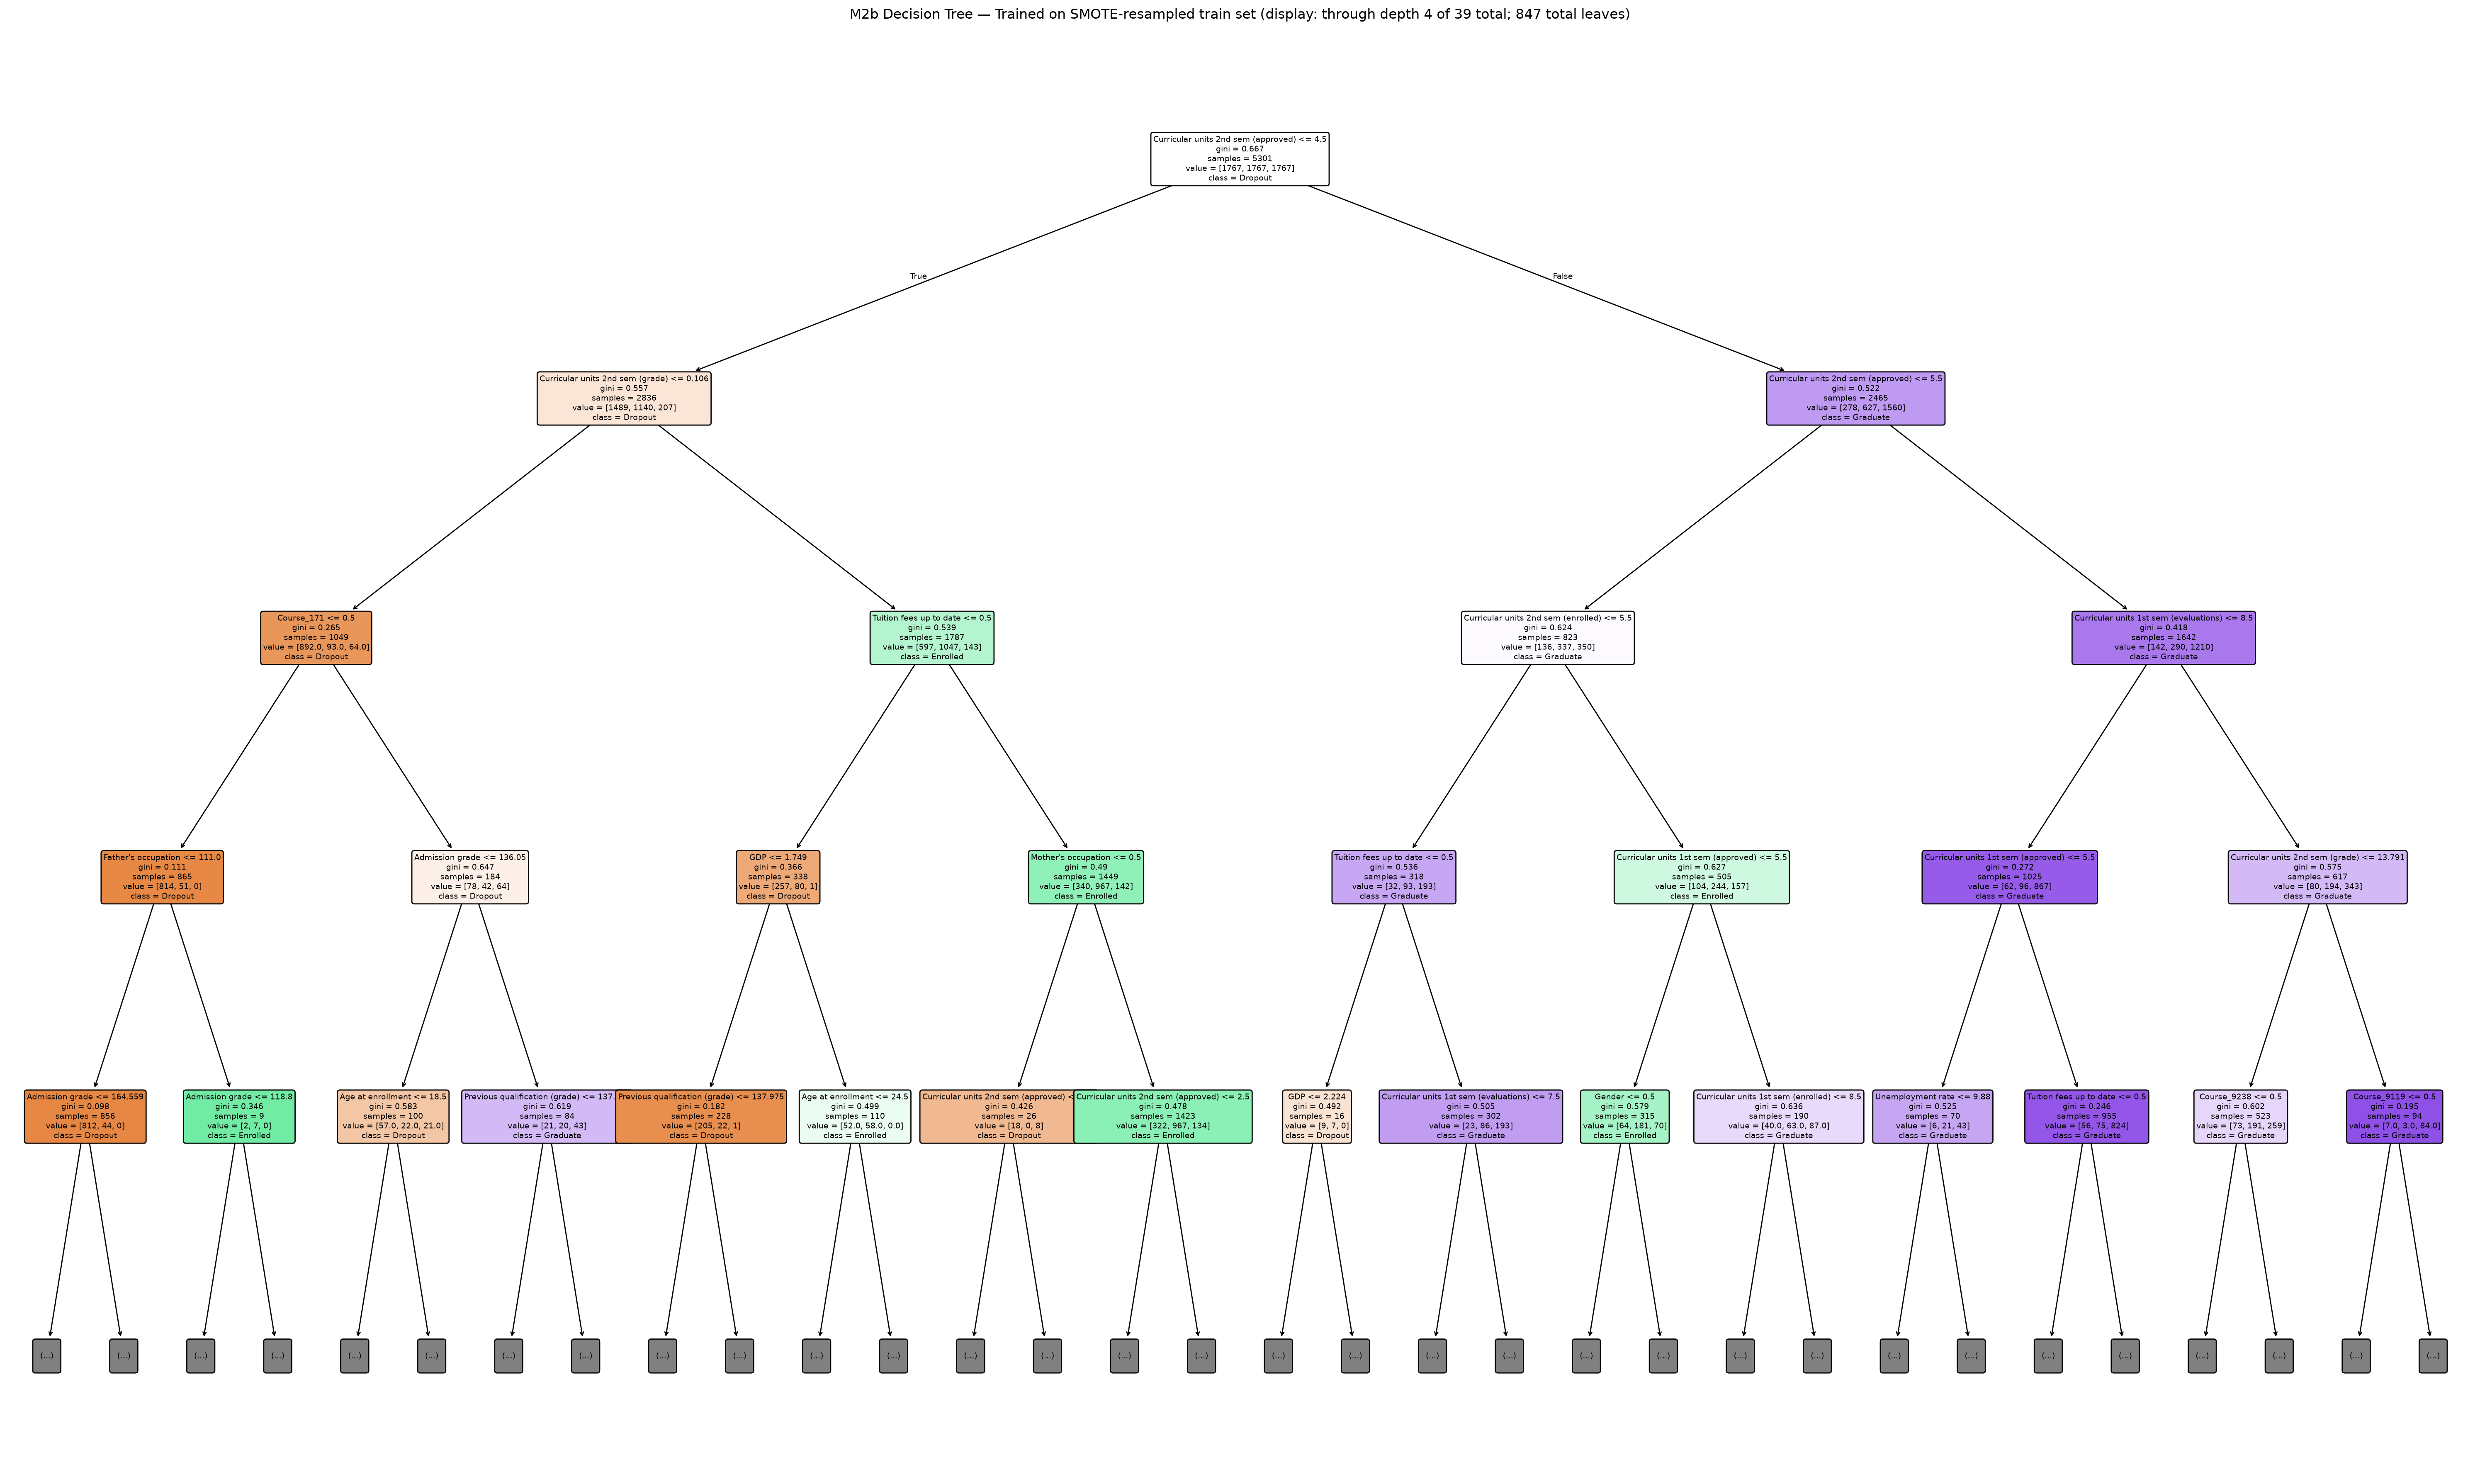
\includegraphics[width=1\textwidth]{D_tree_M2b.png}
  \caption{M2b decision tree displayed through the first four levels.}
  \label{fig:tree-m2b}
\end{figure}

M2b was trained on the SMOTE-resampled training set of 5{,}301 rows and
evaluated exclusively on the original held-out set. Its fitted depth is 39,
with 847 leaves; the display limit does not alter the model.

\begin{figure}[H]
  \centering
  \includegraphics[width=1\textwidth]{D_tree_M2b_full.png}
  \caption{Full M2b decision tree (depth 39, 847 leaves).}
  \label{fig:tree-m2b-full}
\end{figure}

The fitted M2b tree is larger than both M0 and M2a. SMOTE increases the
training set from 3{,}539 to 5{,}301 rows, but this experiment does not isolate
resampled row count as the sole cause of the increased structural complexity.

\subsubsection{Accuracy and error rate}
\label{sec:f2-results}

Table~\ref{tab:f2-main-metrics} reports the full set of held-out test metrics for
M0, M2a, and M2b, together with the change relative to the baseline. Table~
\ref{tab:f2-per-class} reports per-class precision and F1-score, which are not part
of the shared experiment-results artifact schema but are read directly from the two
classification reports.

\begin{table}[H]
\centering
\caption{Held-out test performance: M0 baseline versus M2a and M2b.}
\label{tab:f2-main-metrics}
\begin{tabular}{lrrrrr}
\toprule
\textbf{Metric} & \textbf{M0} & \textbf{M2a} & \textbf{M2b} & \textbf{M2a $-$ M0} & \textbf{M2b $-$ M0} \\
\midrule
Test accuracy        & 0.668927 & 0.650847 & \textbf{0.688136} & $-0.018079$ & \textbf{$+0.019209$} \\
Error rate            & 0.331073 & 0.349153 & \textbf{0.311864} & $+0.018079$ & \textbf{$-0.019209$} \\
Recall (Dropout)      & 0.679577 & 0.679577 & \textbf{0.707746} & $+0.000000$ & \textbf{$+0.028169$} \\
Recall (Enrolled)     & 0.383648 & 0.339623 & \textbf{0.465409} & $-0.044025$ & \textbf{$+0.081761$} \\
Recall (Graduate)     & \textbf{0.764706} & 0.744344 & 0.755656 & $-0.020362$ & $-0.009050$ \\
Precision (macro)     & 0.607642 & 0.584250 & \textbf{0.636513} & $-0.023392$ & \textbf{$+0.028871$} \\
Recall (macro)         & 0.609310 & 0.587848 & \textbf{0.642937} & $-0.021462$ & \textbf{$+0.033627$} \\
F1-score (macro)       & 0.608271 & 0.585409 & \textbf{0.638747} & $-0.022862$ & \textbf{$+0.030475$} \\
ROC-AUC (macro, OvR)   & 0.719456 & 0.705321 & \textbf{0.742122} & $-0.014135$ & \textbf{$+0.022667$} \\
Tree depth / leaves   & 27 / 634 & 28 / 696 & 39 / 847 & - & - \\
\bottomrule
\end{tabular}
\end{table}

\vspace{0.3cm}

\begin{table}[H]
\centering
\caption{Per-class precision and F1-score for M2a and M2b.}
\label{tab:f2-per-class}
\begin{tabular}{lrrrr}
\toprule
\textbf{Class} & \textbf{M2a Precision} & \textbf{M2b Precision} & \textbf{M2a F1} & \textbf{M2b F1} \\
\midrule
Dropout   & 0.6328 & \textbf{0.7003} & 0.6553 & \textbf{0.7040} \\
Enrolled  & 0.3234 & \textbf{0.4044} & 0.3313 & \textbf{0.4327} \\
Graduate  & 0.7966 & 0.8048 & 0.7696 & 0.7795 \\
\bottomrule
\end{tabular}
\end{table}

Notably, M2b does not merely predict \textit{Enrolled} more often at the expense of
precision: its \textit{Enrolled} precision \emph{also} increases relative to M2a
(from $0.3234$ to $0.4044$), so that when M2b predicts a student as
\textit{Enrolled} it is more likely to be correct, not merely more willing to
guess that label. This is the reason the \textit{Enrolled} F1-score of M2b
($0.4327$) is substantially higher than that of M2a ($0.3313$).

\subsubsection{Why this does (or does not) improve the result}
\label{sec:f2-discussion}

\textbf{M2a does not achieve the goal of this experiment on this split.} Test
accuracy falls by $1.81$ percentage points relative to M0; recall on
\textit{Dropout} is unchanged, recall on \textit{Enrolled} falls by $4.40$
percentage points, and recall on \textit{Graduate} falls by $2.04$ percentage
points. Because both overall accuracy and the recall of the classes this
improvement is meant to prioritize either fall or stay flat, there is no evidence
from the held-out test set that \texttt{class\_weight='balanced'} alone improves
M0 in this configuration. This negative result is reported in full rather than
omitted, since selectively reporting only favorable configurations would
misrepresent the effectiveness of class weighting for this dataset.

\textbf{On this held-out split, M2b improves the target metrics.} Recall on
\textit{Enrolled} rises from
$0.383648$ to $0.465409$ (61/159 $\rightarrow$ 74/159 students correctly
identified), and recall on \textit{Dropout} rises from $0.679577$ to $0.707746$
(193/284 $\rightarrow$ 201/284). \textit{Graduate} recall falls only marginally,
from $0.764706$ to $0.755656$. All macro-averaged metrics improve simultaneously
(macro F1: $0.608271 \rightarrow 0.638747$; macro recall:
$0.609310 \rightarrow 0.642937$). This is consistent with the intended mechanism
of SMOTE: \textit{Enrolled} has the fewest original observations in the training
data, so synthetic interpolation in its feature-space neighbourhood gives the tree
more candidate split points with which to separate \textit{Enrolled} from the
other two classes. This is a mechanistic explanation specific to this experiment,
not a causal claim that every dataset or split would show an identical gain. It is
also worth noting explicitly that M2b's tree is substantially larger than M0's
(depth 39 versus 27, 847 versus 634 leaves): the recall improvement is not the
result of a simpler, more interpretable tree, since simplification is not the
objective of this improvement method (that objective is addressed separately by
Improvement Method 1, cost-complexity pruning).

An overall test-accuracy \emph{increase} for M2b is a welcome but secondary
finding here. Because this experiment specifically targets class-wise detection,
the primary evidence is the per-class recall table above. On this held-out set,
M2b has higher Dropout and Enrolled recall than both M0 and M2a.

\subsubsection{Limitation: vanilla SMOTE on encoded categorical features}
\label{sec:f2-limitation}

The shared preprocessing pipeline one-hot encodes only four
categorical groups (\textit{Marital Status}, \textit{Application mode},
\textit{Course}, \textit{Previous qualification}); the remaining high-cardinality
categorical variables - \textit{Mother's/Father's qualification},
\textit{Mother's/Father's occupation}, \textit{Nacionality} (nominal), and
\textit{Application order} (ordinal) - are retained as integer codes. Vanilla
SMOTE treats every input feature as continuous and linearly interpolates between a
sample and its nearest neighbours, which can in principle generate values that do
not correspond to any real category.

This effect was measured directly on the 1{,}762 synthetic rows that M2b actually
uses for training, rather than assumed.

\begin{table}[H]
\centering
\caption{Out-of-vocabulary category codes among the 1{,}762 synthetic rows, for
the six integer-coded categorical columns.}
\label{tab:f2-code-audit}
\begin{tabular}{llrr}
\toprule
\textbf{Column} & \textbf{Type} & \textbf{Non-integer rate} & \textbf{Out-of-vocabulary rate} \\
\midrule
Mother's qualification & nominal & 0.00\% & 3.01\% \\
Father's qualification & nominal & 0.00\% & 2.89\% \\
Mother's occupation     & nominal & 0.00\% & 1.19\% \\
Father's occupation     & nominal & 0.00\% & 2.04\% \\
Nacionality              & nominal & 0.00\% & 2.38\% \\
Application order        & ordinal & 0.00\% & 0.00\% \\
\bottomrule
\end{tabular}
\end{table}

\vspace{0.3cm}

\begin{table}[H]
\centering\small
\caption{Interpolation outcome for the four one-hot-encoded groups, measured on
the 1{,}762 synthetic rows. Percentages are row-wise: every synthetic row falls
into exactly one of the first three columns.}
\label{tab:f2-onehot-audit}
\begin{tabular}{lrrrrr}
\toprule
\textbf{One-hot group} & \textbf{All-zero} & \textbf{Multi-hot} & \textbf{Fractional} & \textbf{Any violation} & \textbf{Valid one-hot} \\
\midrule
Marital Status          & 14.7\% & 0.0\% & 0.0\% & 14.7\% & 85.3\% \\
Application mode        & 65.4\% & 0.0\% & 0.0\% & 65.4\% & 34.6\% \\
\textbf{Course}          & \textbf{83.0\%} & 0.0\% & 0.0\% & \textbf{83.0\%} & 17.0\% \\
Previous qualification  & 24.8\% & 0.0\% & 0.0\% & 24.8\% & 75.2\% \\
\bottomrule
\end{tabular}
\end{table}

The two measurements must be read differently.

For the \textbf{six integer-coded columns}, the audit detects no non-integer
values whatsoever in the synthetic data. This result must \emph{not} be
interpreted as "SMOTE does not affect these columns": it is very plausible that
interpolated fractional values were truncated to integers during
\texttt{fit\_resample()}'s dtype-restoration step, which would make this
measurement, at the level of raw values, unable to detect the interpolation that
still occurred. Even where a value is an integer, it can still fail to correspond
to any real category - and the out-of-vocabulary-rate column above shows exactly
this: up to $3.01\%$ of synthetic values for \textit{Mother's qualification} are
integer codes that never appear anywhere in the real training data.

For the \textbf{four one-hot groups}, the measurement is unambiguous and fully
quantitative. \texttt{imbalanced-learn} 0.14.2's internal \texttt{ArraysTransformer}
restores the output DataFrame to the exact dtype of its input columns via
\texttt{astype()} \citep{imblearn_arrays_transformer}. Because the dummy columns
produced have integer dtype, any fractional value produced
by SMOTE's linear interpolation between two different one-hot vectors is truncated
toward zero rather than rounded. Given that a convex combination of two valid
one-hot vectors can never itself exceed 1 in any single component, this truncation
can only push a component down to $0$, never up past $1$: the audit accordingly
finds a fractional-component rate of $0.0\%$ and a multi-hot rate of $0.0\%$ in
every group, and \emph{100\% of the observed violations are all-zero vectors}
(no category active) rather than any mixture of multiple categories. \textit{Course}'s high cardinality is a plausible contributor to its high all-zero violation rate ($83.0\%$) under this encoding-and-restoration path. The audit does not isolate category count as the sole cause.

This is a documented limitation of vanilla SMOTE when applied to mixed
continuous/categorical representations; the official \texttt{imbalanced-learn}
documentation recommends \texttt{SMOTENC} for exactly this situation
\citep{imblearn_oversampling_guide}. Vanilla SMOTE was retained as one of the group's selected class-imbalance experiments. The assignment brief suggests handling class imbalance as a possible improvement direction but does not mandate SMOTE specifically. The M2b results reported above should
therefore be read together with this limitation: the recall and precision
improvements are measured on the real, untouched held-out test set, but
part of the synthetic training data the tree learns from does not represent a
"valid" student under the true meaning of the affected categorical columns.

\subsubsection{Accuracy-recall trade-off}
\label{sec:f2-tradeoff}

In a class-imbalanced classification problem, overall accuracy alone cannot be the
sole acceptance criterion. A model may legitimately trade a reduction in overall
accuracy for less majority-class dominance; when this happens,
per-class recall - not a return to M0's accuracy figure - is the correct measure
of success.

M2a illustrates that this trade-off is not automatic: its accuracy falls
\emph{and} its \textit{Enrolled} recall falls, so the result is reported plainly
rather than selectively. M2b, by contrast, is not a trade-off at all on this
held-out split: it simultaneously increases test accuracy ($0.668927 \rightarrow 0.688136$), \textit{Dropout}
recall, and \textit{Enrolled} recall, at the cost of a $0.90$ percentage-point
reduction in \textit{Graduate} recall. If the evaluation priority is detecting
students who are at risk of dropping out or remaining indefinitely enrolled, M2b
is therefore the preferable configuration among M0, M2a, and M2b on this held-out
split.

These findings are drawn from a single fixed held-out split, and the synthetic
portion of M2b's training data carries the categorical-representation limitation
discussed above. Before any real-world deployment, results should be validated
across multiple splits or cohorts, \texttt{SMOTENC} should be considered as an
additional experiment, and performance disparities across the dataset's
sensitive groups should be examined. Within the scope of this experiment and
the project's shared data split, however, M2b answers the improvement question
affirmatively: the
minority \textit{Enrolled} class and the \textit{Dropout} class are both
recognized more reliably when SMOTE is applied strictly to the training split.

\subsubsection{Conclusion}
\label{sec:f2-conclusion}

Balanced class weighting (M2a) does not improve upon the M0 baseline on this
held-out test set: overall accuracy, \textit{Enrolled} recall, and
\textit{Graduate} recall all fall, while \textit{Dropout} recall is unchanged.
Applying SMOTE to the training split only (M2b) increases \textit{Enrolled}
recall by $8.18$ percentage points and \textit{Dropout} recall by $2.82$
percentage points relative to M0, while simultaneously raising \textit{Enrolled}
precision from $0.3567$ to $0.4044$ and lowering the overall error rate from
$0.331073$ to $0.311864$. M2b is therefore adopted as the more successful
class-imbalance configuration within the scope of this experiment. M2a is
retained in this report rather than discarded, both for transparency - not every
class-balancing technique improves a given model on a given dataset - and to
document, alongside M2b, the quantitative categorical-representation limitation
of vanilla SMOTE rather than presenting only favorable figures.

% Owner: Role E. NOT translated yet -- structural skeleton only.
%
% Source material: notebooks/05_improve_features.ipynb markdown cells
% (already fact-checked -- progress/A.md 2026-08-30 audit: 0 errors out
% of ~12 checked numeric claims; the notebook even self-verifies its own
% numbers against outputs/results.csv before printing "PASS"). There is
% no separate docs/report_draft_f3_*.md file -- render the notebook to
% read it comfortably if needed:
%   jupyter nbconvert --to markdown notebooks/05_improve_features.ipynb
%
% Brief requires, for EACH improvement method (Section 3.4.f):
%   - Description of the method
%   - Modified tree or model setting
%   - Accuracy and error rate
%   - Explanation of why the method improves (or does not improve) the result
%
% Figures already committed and ready to reference (do not rename):
%   figures/E_feature_importance.png  -- M0 vs M3 top-10 Gini importance
%   figures/E_tree_M3.png             -- M3 tree
%   figures/E_cm_M3.png               -- M3 confusion matrix
%
% IMPORTANT: when citing "most important features," always source the
% number from outputs/E_feature_importance_comparison.csv (this project's
% own M0/M3 Gini importance), NOT from docs/02-DATASET-VA-CONG-VIEC.md
% Section A5 (the original paper's Random Forest/XGBoost/LightGBM/CatBoost
% permutation importance -- a different algorithm on a different model).
% Conflating the two was exactly the error Role A found and fixed in its
% own g_comparison.tex source draft -- e.g. "Curricular units 1st sem
% (approved)" is in the paper's top-5 but ranks 9th in this project's own
% M0 tree. Section c_dataset.tex above already states the corrected M0
% top-5 explicitly if you need to cross-check.

\subsection{f.3 Improvement Method 3: Feature Selection for Early Warning}
\label{sec:f3}

\subsubsection{Method description}

\todo{Describe the method: drop exactly the 12 semester-outcome columns (all six \texttt{Curricular units 1st sem (\ldots)} and six \texttt{Curricular units 2nd sem (\ldots)} columns), keep the remaining 24 original features including the 3 macroeconomic variables (known at enrollment time), and train an unconstrained \texttt{DecisionTreeClassifier(random\_state=42)} exactly like M0 so the only experimental difference is feature availability.}

\subsubsection{Modified tree / model setting}

\begin{figure}[H]
  \centering
  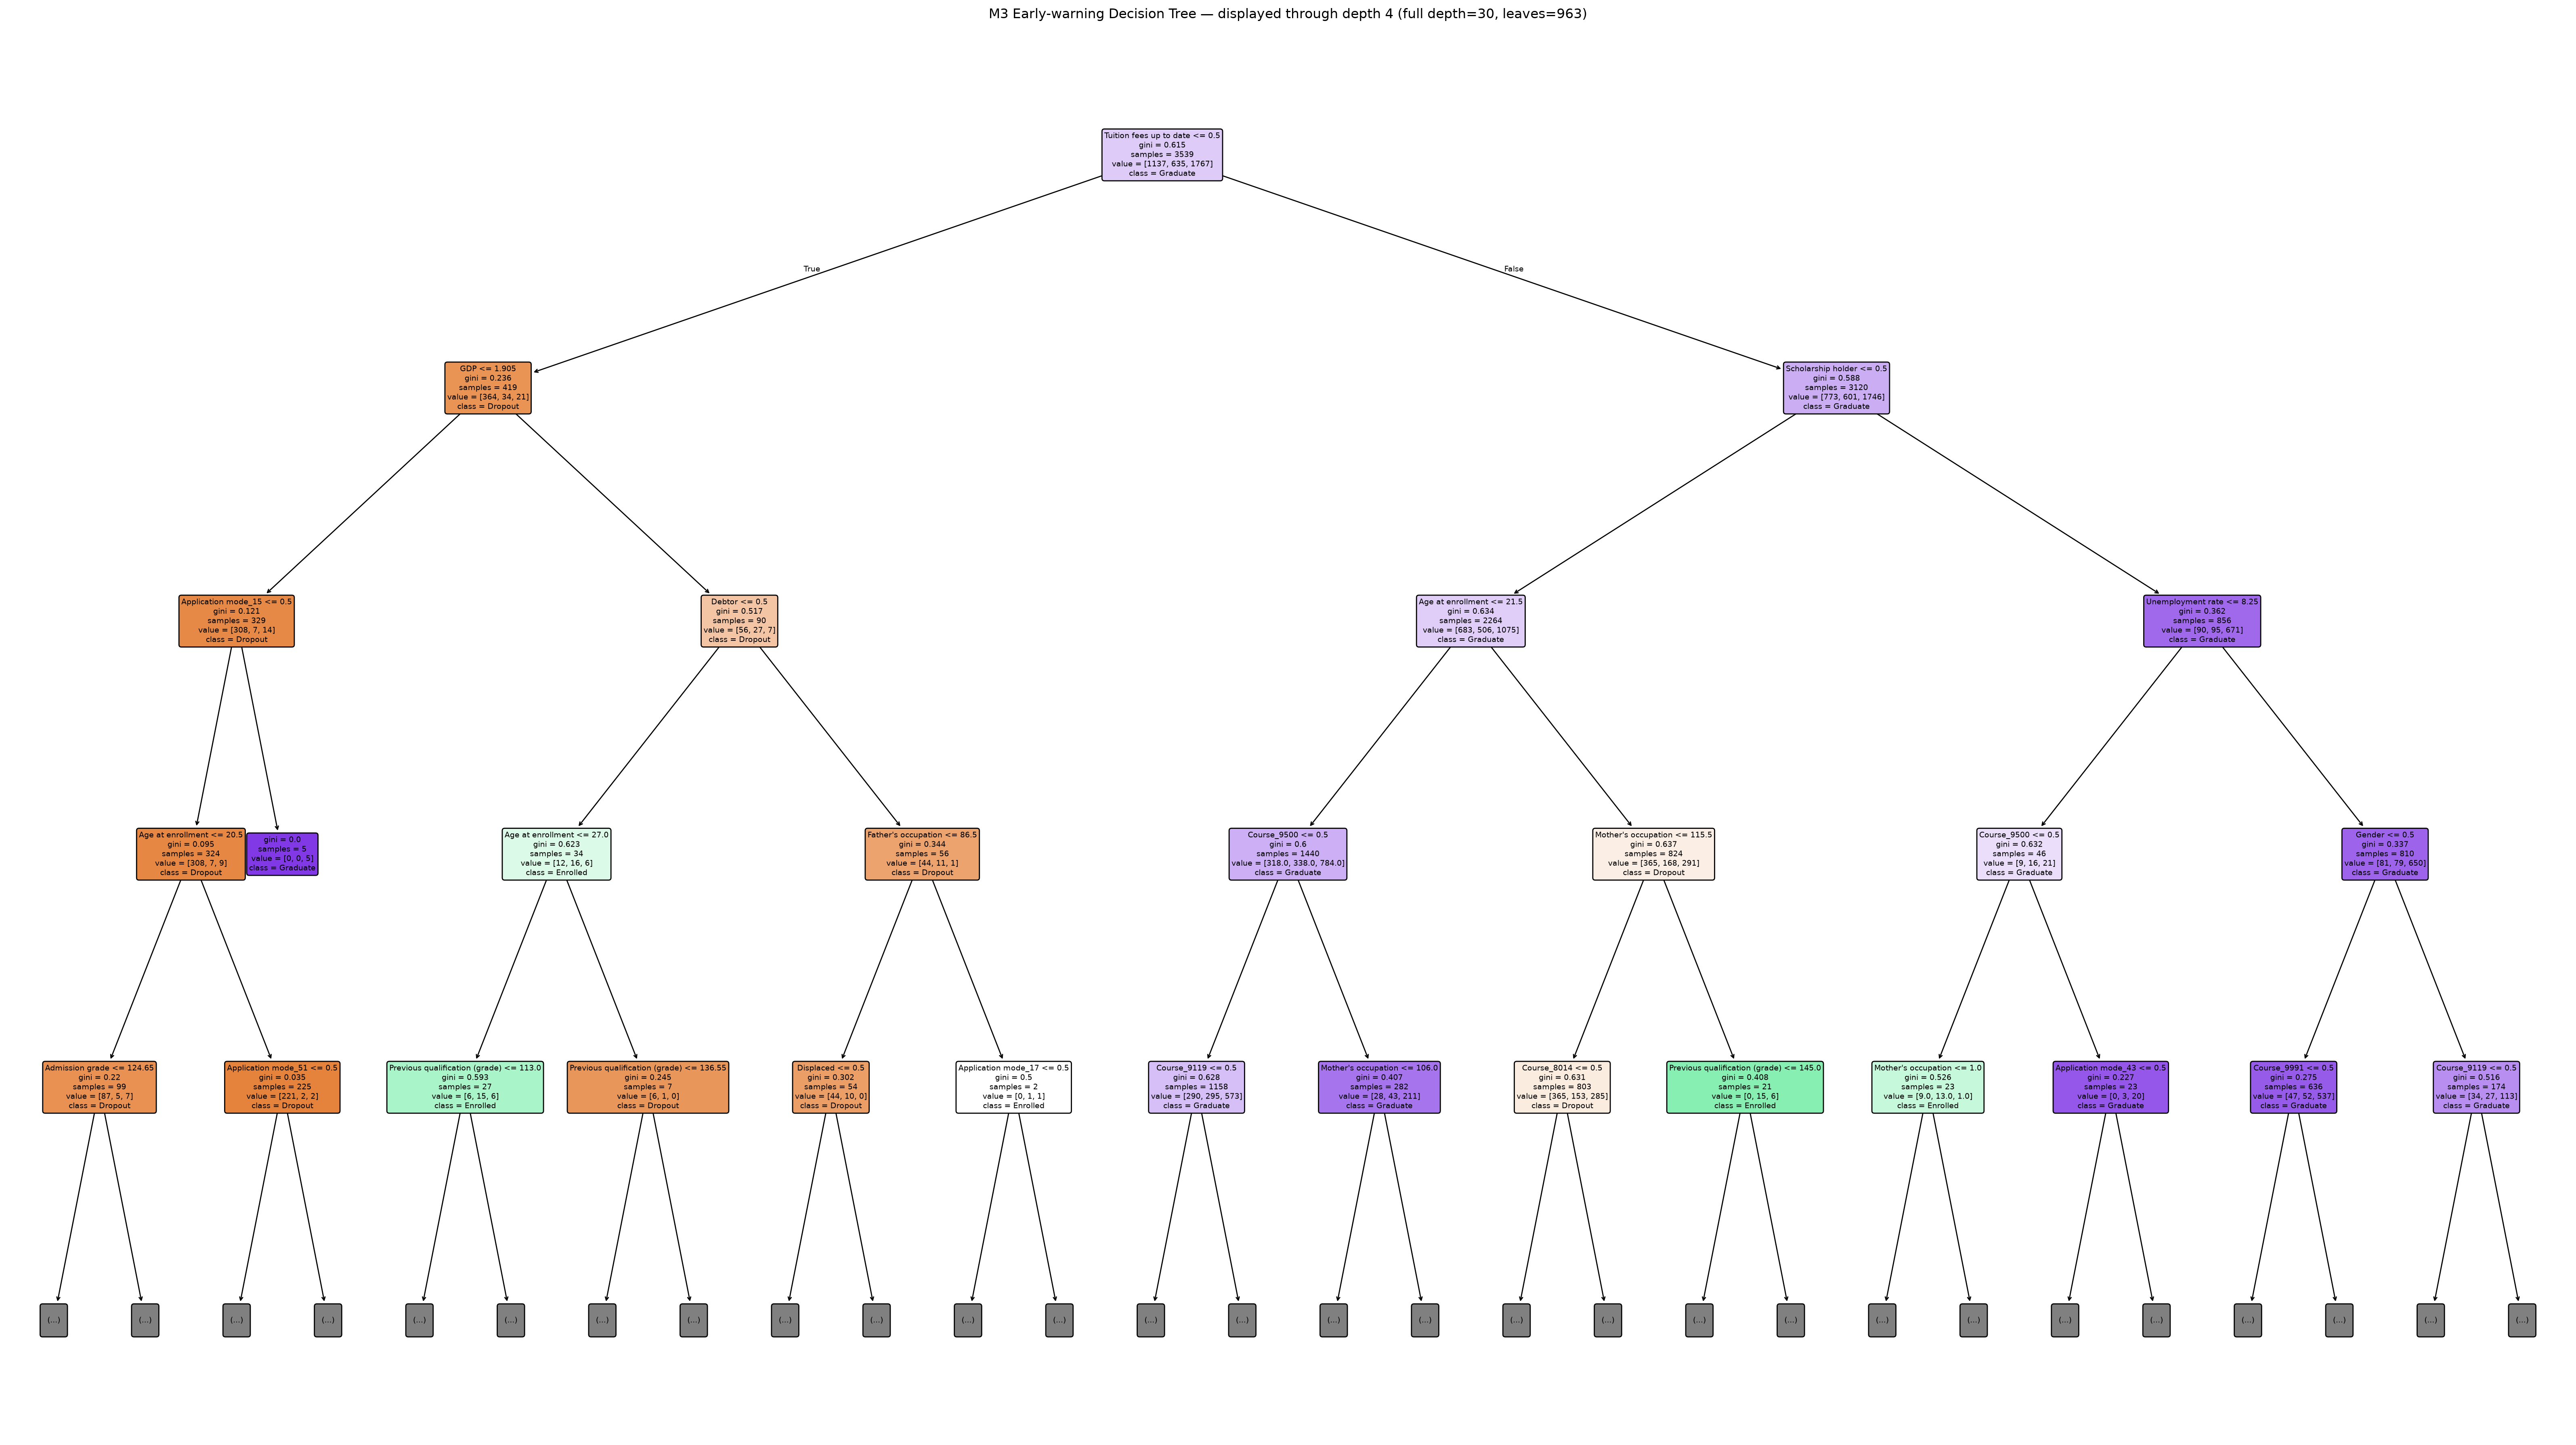
\includegraphics[width=0.75\textwidth]{E_tree_M3.png}
  \caption{\todo{Caption: M3 tree (state depth/leaves from \texttt{outputs/results.csv}).}}
\end{figure}

\begin{figure}[H]
  \centering
  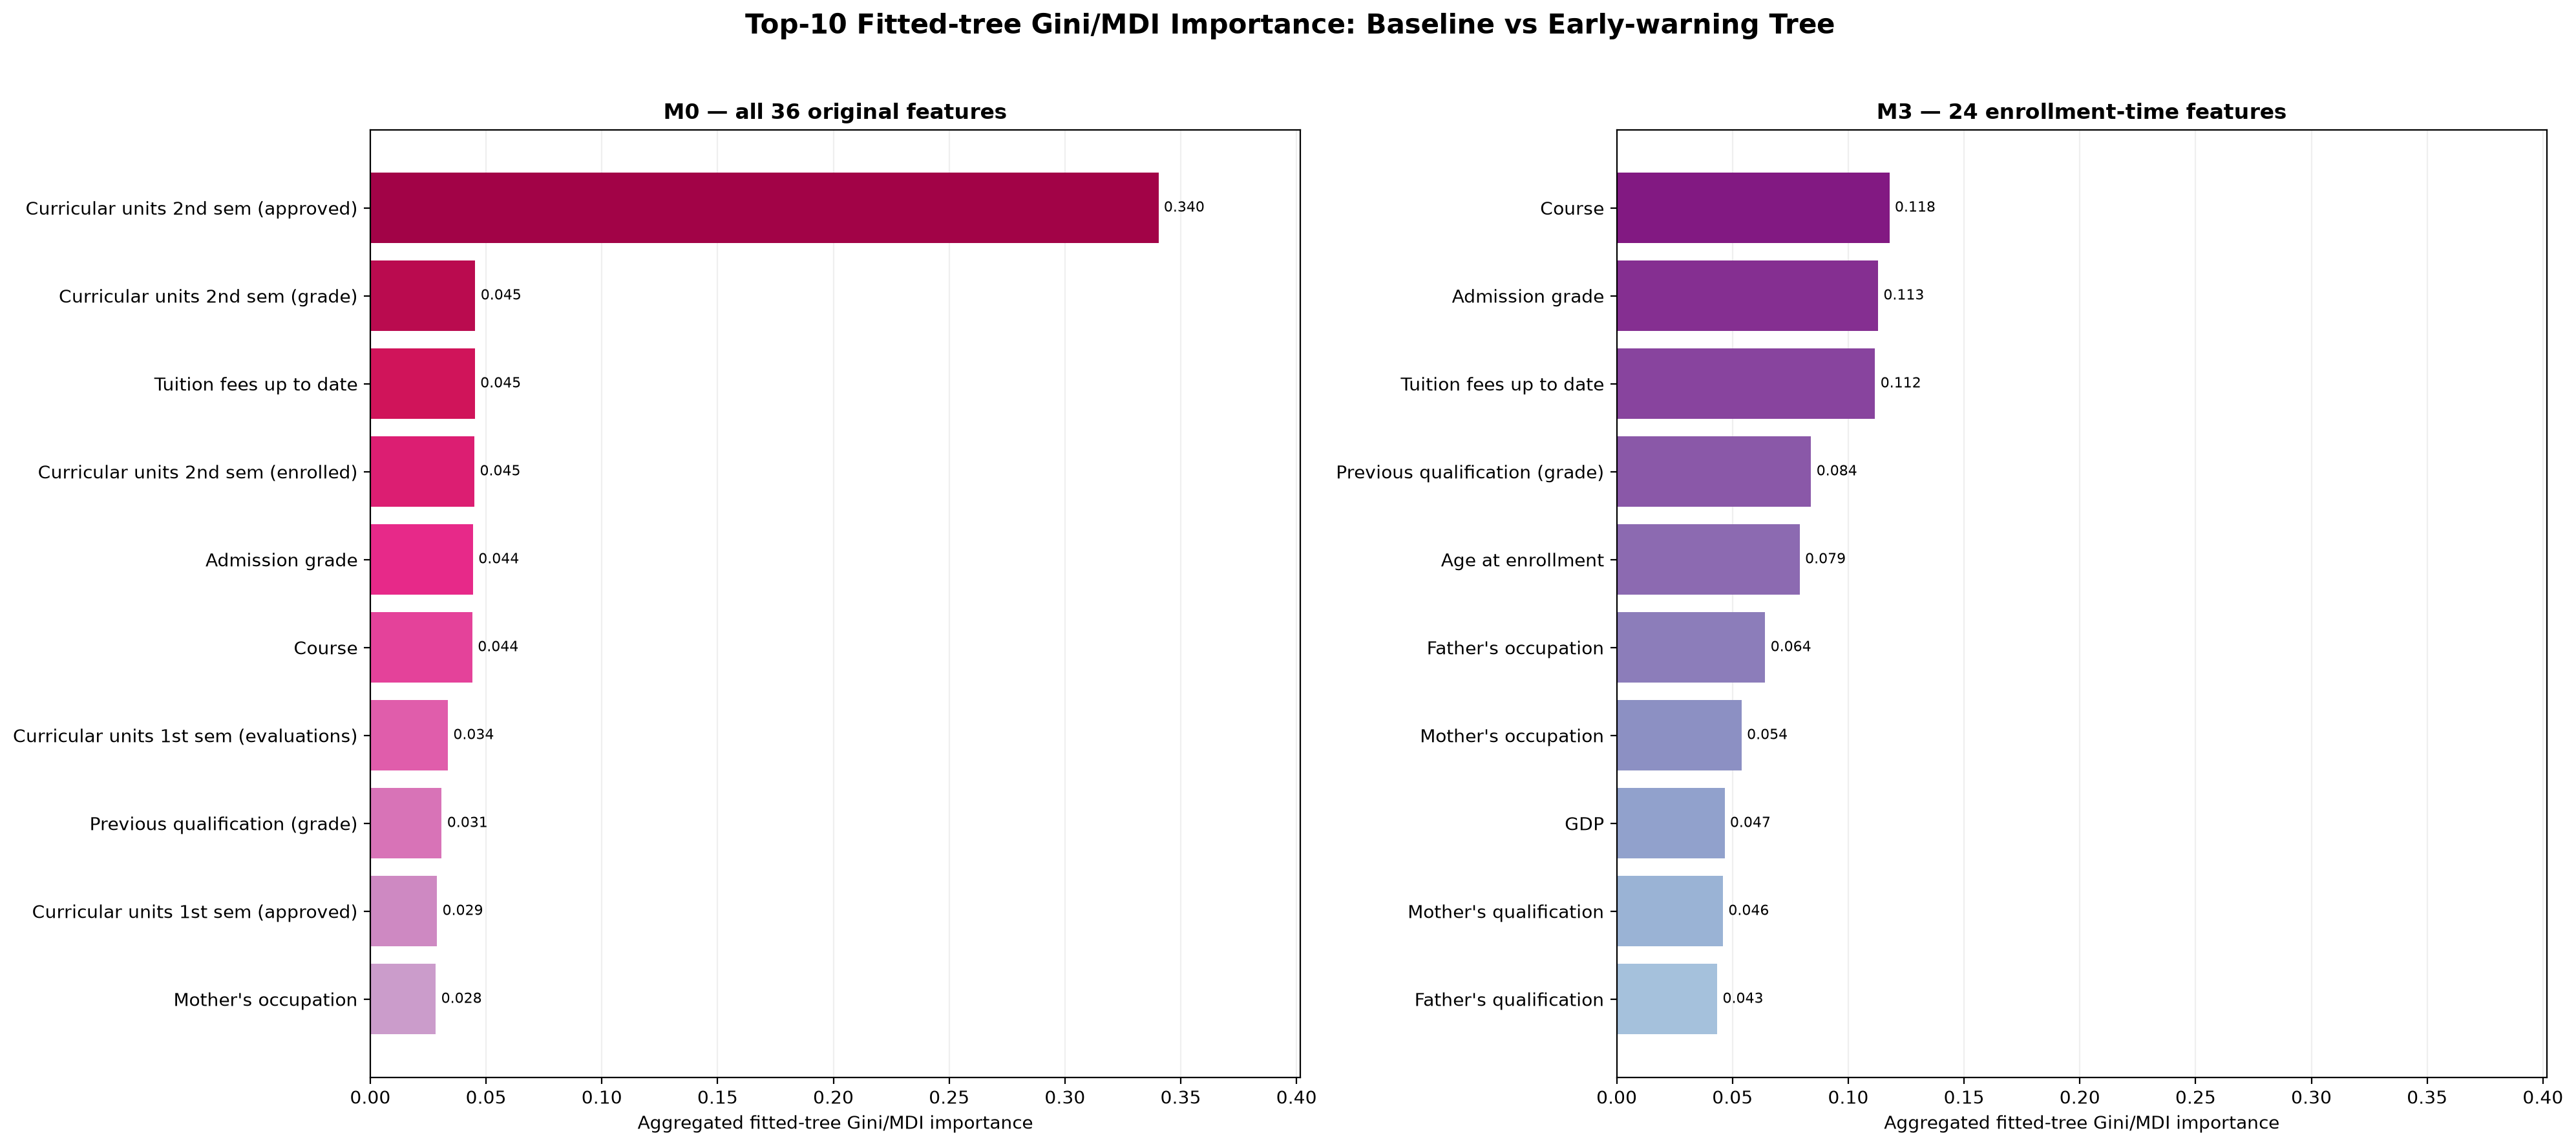
\includegraphics[width=\textwidth]{E_feature_importance.png}
  \caption{\todo{Caption: top-10 Gini feature importance, M0 (all 36 original features) vs.\ M3 (24 retained features) side by side, one-hot dummy importances summed back to their original UCI feature name for a fair comparison.}}
\end{figure}

\subsubsection{Accuracy and error rate}

\todo{Report M3's test\_acc / error\_rate / F1 macro against M0 from \texttt{outputs/results.csv}, and the confusion matrix below.}

\begin{figure}[H]
  \centering
  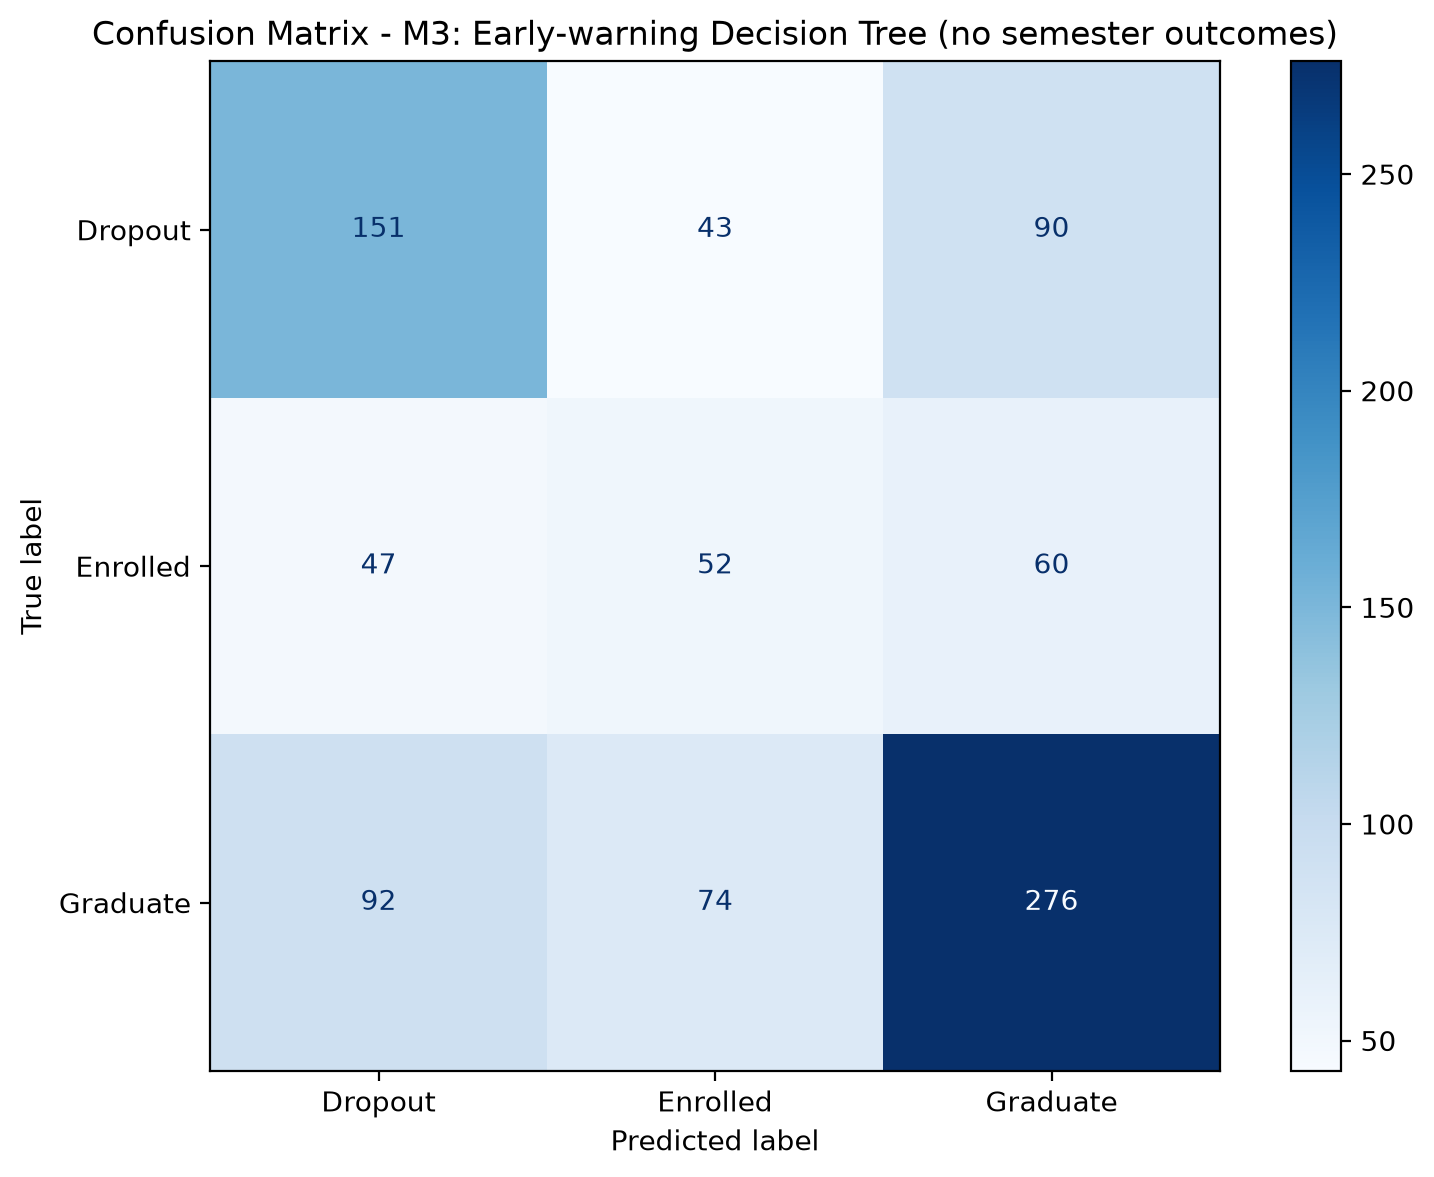
\includegraphics[width=0.6\textwidth]{E_cm_M3.png}
  \caption{\todo{Caption: M3 confusion matrix on the same 885-sample held-out test set as every other model.}}
\end{figure}

\subsubsection{Why this does not improve accuracy --- and why that is expected}

\todo{Explain plainly that accuracy drops substantially (this is the intended finding, not a failure): the 12 dropped columns include several of M0's strongest actual Gini-importance features (see \texttt{outputs/E\_feature\_importance\_comparison.csv} -- \texttt{2nd sem approved} is M0's single most important feature by a wide margin), all of which are only known after a semester ends. State the trade-off explicitly: M0 is more accurate but only actionable after the fact; M3 is less accurate but is the only model of the four that is actually usable at enrollment time for early, preventive intervention. Cite \citep{martins2021early} here if used as background for the early-prediction framing.}


% Final section; all metrics and model-complexity values were checked against
% the canonical comparison and model-specific experiment artifacts.

\section{Comparison of Results}
\label{sec:g}

\subsection{Overall comparison table}

\begin{table}[H]
  \centering
  \caption{All 5 models on the shared 885-sample held-out test set}
  \label{tab:g1}
  \resizebox{\textwidth}{!}{%
  \begin{tabular}{@{}lrrrrrrrrr@{}}
    \toprule
    Model & Test acc & Error & F1 macro & ROC-AUC & Rec.\ Dropout & Rec.\ Enrolled & Rec.\ Graduate & Depth & Leaves \\
    \midrule
    M0 (baseline)        & 0.6689 & 0.3311 & 0.6083 & 0.7195 & 0.6796 & 0.3836 & 0.7647 & 27 & 634 \\
    M1 (pruning)          & \textbf{0.7559} & \textbf{0.2441} & \textbf{0.6729} & \textbf{0.8477} & 0.6866 & 0.3459 & \textbf{0.9480} & \textbf{5} & \textbf{17} \\
    M2a (class\_weight)   & 0.6508 & 0.3492 & 0.5854 & 0.7053 & 0.6796 & 0.3396 & 0.7443 & 28 & 696 \\
    M2b (SMOTE)           & 0.6881 & 0.3119 & 0.6387 & 0.7421 & \textbf{0.7077} & \textbf{0.4654} & 0.7557 & 39 & 847 \\
    M3 (early warning)    & 0.5412 & 0.4588 & 0.4931 & 0.6254 & 0.5317 & 0.3270 & 0.6244 & 30 & 963 \\
    \bottomrule
  \end{tabular}%
  }
\end{table}

\begin{figure}[H]
  \centering
  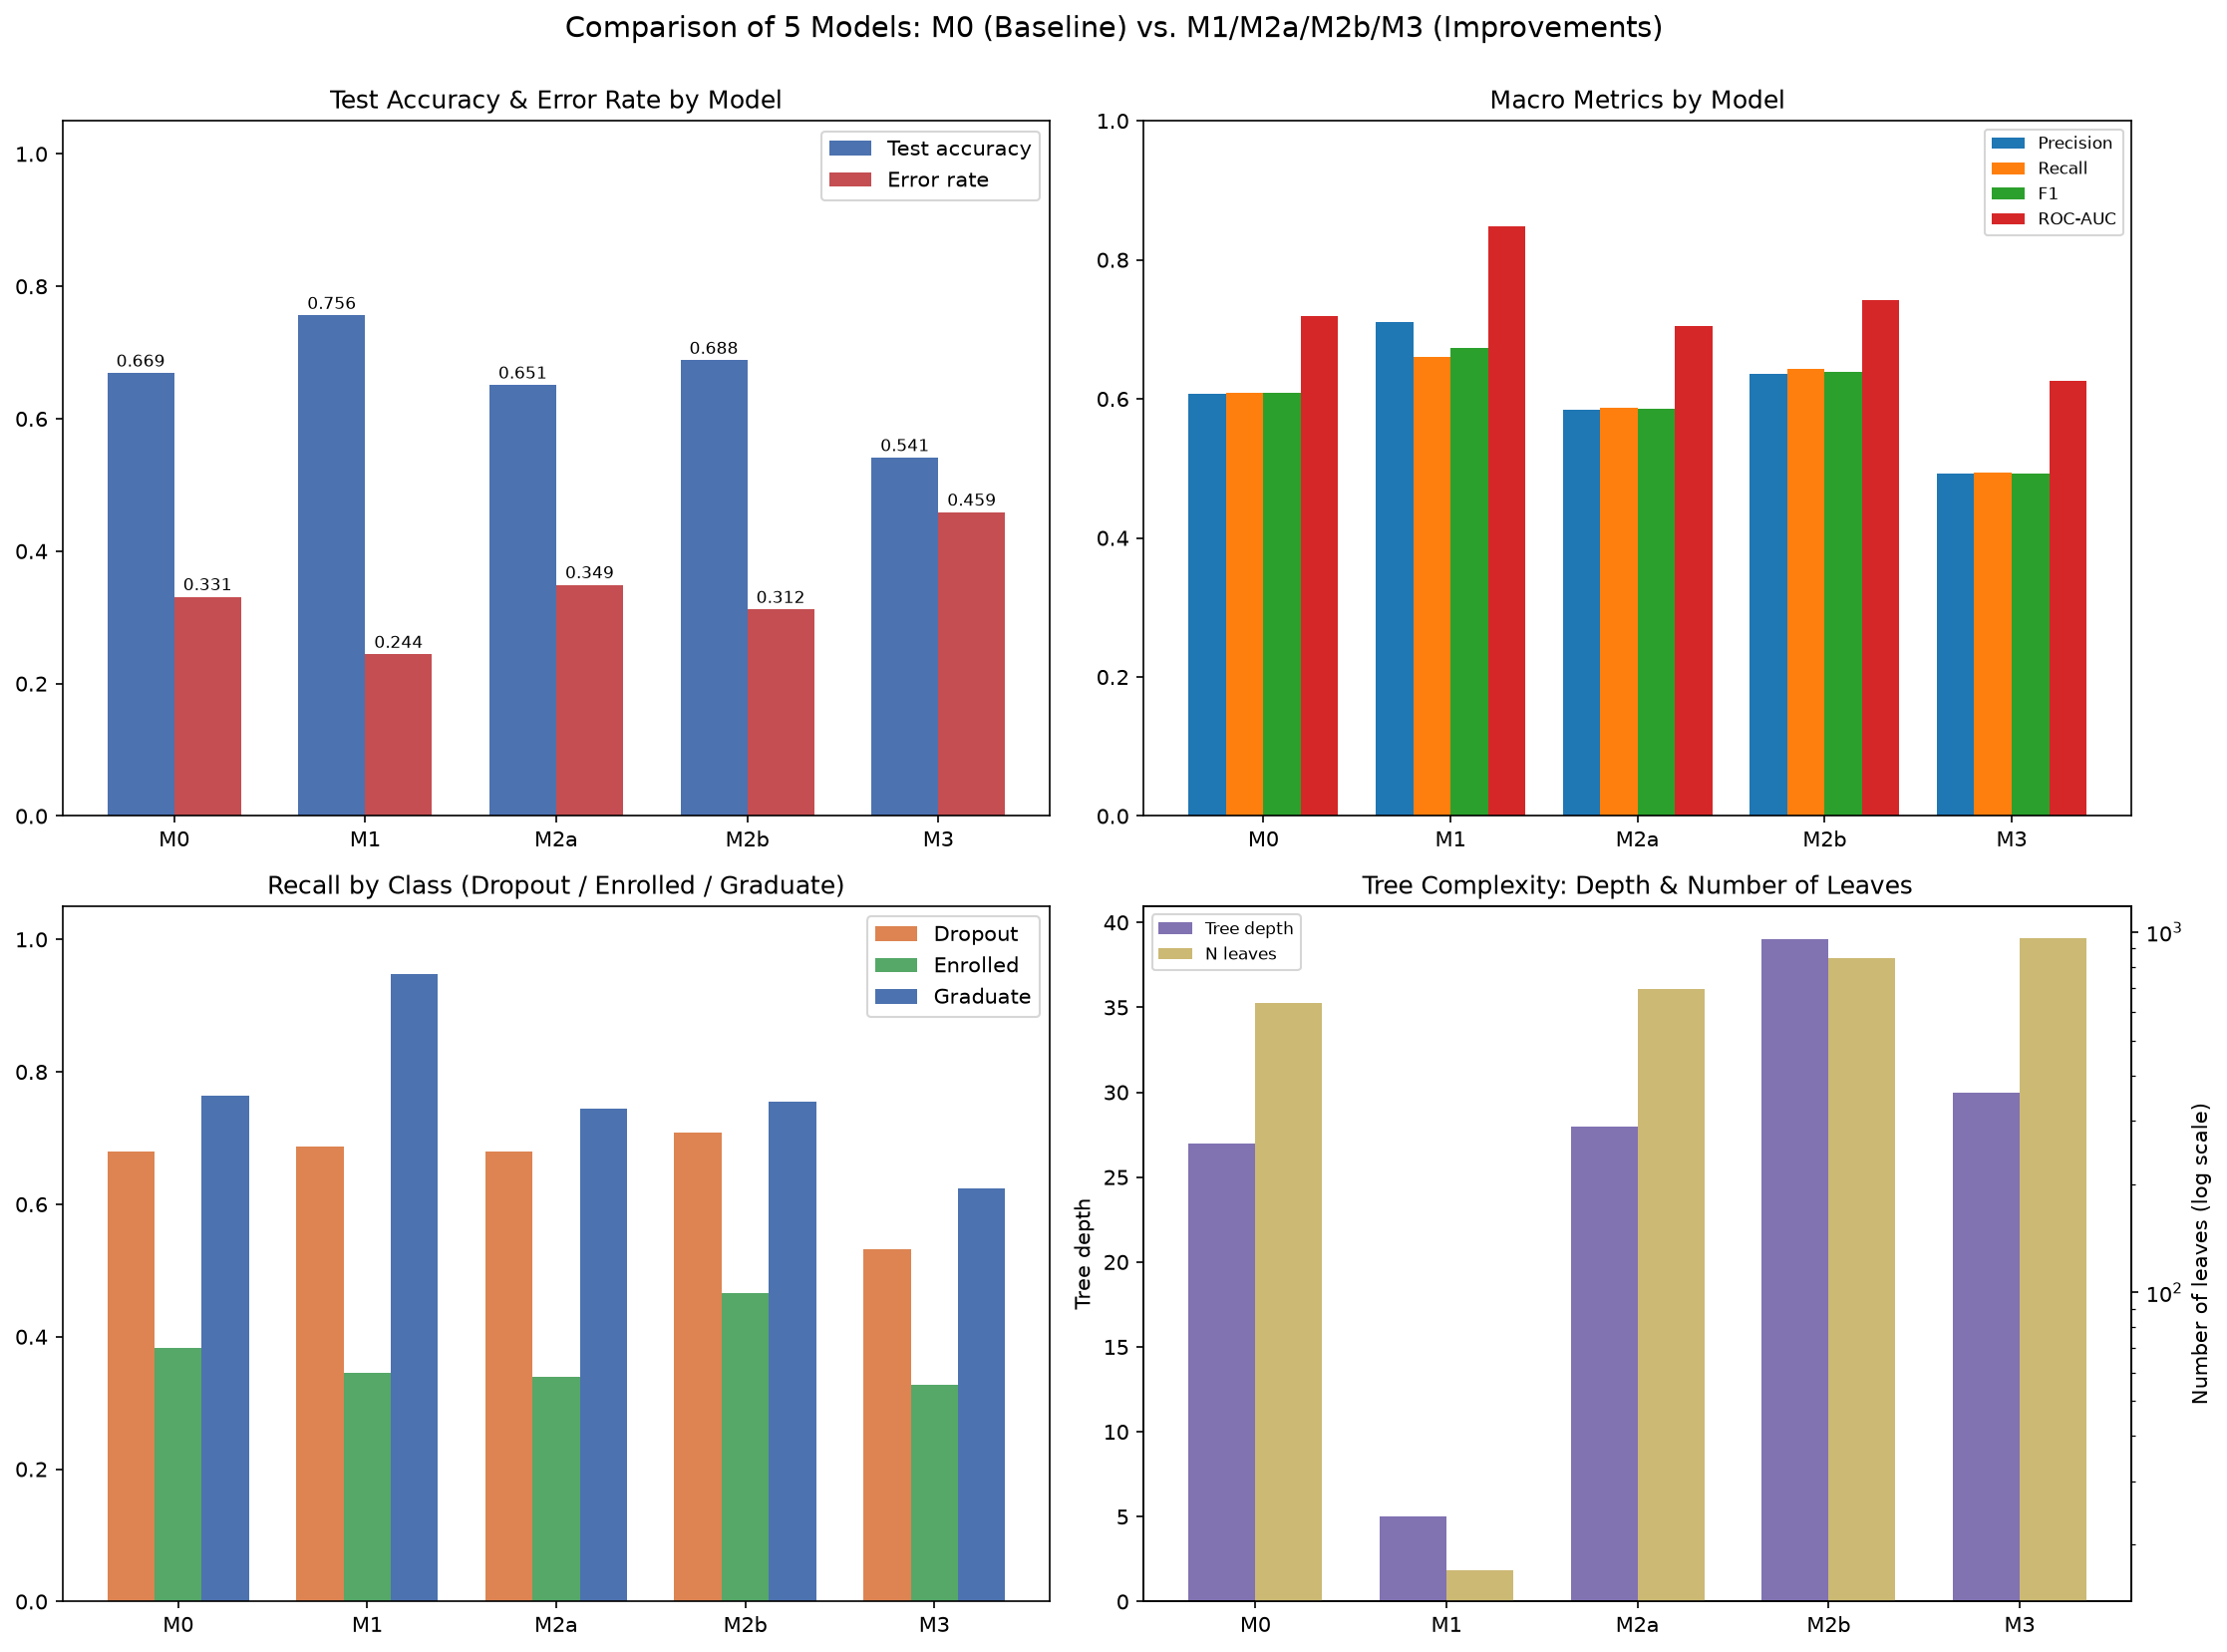
\includegraphics[width=\textwidth]{comparison.png}
  \caption{Four-panel comparison of M0-M1-M2a-M2b-M3 on the same
    held-out test set (885 samples).}
  \label{fig:g1}
\end{figure}

Reading the four panels: top-left (test accuracy and error rate) shows
M1 highest and M3 lowest; top-right (the four macro metrics: Precision,
Recall, F1, ROC-AUC) shows M1 leading on all four; bottom-left (per-class
recall) shows M2b dominating on Dropout and Enrolled while M1 dominates
on Graduate; bottom-right (tree complexity, leaf count on a log scale)
shows M1 far more compact than the other four models.

\subsection{Comparing each improvement against the baseline}

\textbf{M1 (Pruning) improves almost every aggregate metric.} Test
accuracy rises from 0.6689 to 0.7559 (\textbf{+8.70 percentage points}),
error rate drops from 33.11\% to 24.41\%, F1 macro rises 6.47 points, and
ROC-AUC macro rises 12.82 points. At the same time, complexity drops
sharply: depth 27$\to$5, leaves 634$\to$17 (\textbf{about 37$\times$
fewer}). This is a favorable result: aggregate performance and structural
simplicity both improve, although Enrolled recall decreases slightly
(0.3836$\to$0.3459, $-3.77$ points). Accuracy was the prespecified CV
criterion for selecting \texttt{ccp\_alpha}/\texttt{max\_depth}/
\texttt{min\_samples\_leaf}; because that criterion does not explicitly
protect minority-class recall, it can favor the majority Graduate class
whenever doing so raises the total number of correct predictions.

M2 (Class Imbalance) gives two opposite results, consistent with the
experimental nature of this improvement. M2a
(\texttt{class\_weight='balanced'}) \textbf{does not improve} M0 on this
test set: test accuracy drops 1.81 points, and even Enrolled recall, the
metric this technique targets, also drops (0.3836$\to$0.3396). In
contrast, M2b (SMOTE on train only) improves both overall accuracy
(+1.92 points) and the recall of the two hardest classes: Dropout recall
+2.82 points, Enrolled recall \textbf{+8.18 percentage points} (61/159
$\to$ 74/159 Enrolled students correctly identified), at the cost of a
slight 0.90-point drop in Graduate recall. M2b also raises Enrolled
precision relative to M0 (0.3567$\to$0.4044), so the higher recall does
not simply come from the model predicting Enrolled more often. Vanilla
SMOTE on encoded categorical features still has the quantitative limitations
documented in Section~\ref{sec:f2-limitation}, so this result is best read as
an improvement on this particular held-out set rather than a guarantee for a
new cohort or institution.

\textbf{M3 (Early Warning) drops performance substantially, and this is
the expected result, not a failure.} Test accuracy falls from 0.6689 to
0.5412 (\textbf{$-12.77$ percentage points}), F1 macro falls 11.52
points. A model-grounded explanation comes from M0's own tree rather than
the original paper: by M0's Gini feature importance, 3 of the top
5 features are \texttt{2nd sem approved} (rank~1, importance 0.340, over
a third of the whole tree's total importance), \texttt{2nd sem grade}
(rank~2, 0.045), and \texttt{2nd sem enrolled} (rank~4, 0.045). All
three fall inside the 12 columns dropped in M3 because they are only
known \emph{after} the second semester ends. The other two features in
M0's real top-5, \texttt{Tuition fees up to date} (rank~3) and
\texttt{Admission grade} (rank~5), are retained in M3 because they are
treated as available at enrollment under this study's feature-availability
assumption. The importance ranking is associative rather than causal, but the
held-out performance gap is consistent with the loss of
\texttt{2nd sem approved}, which alone accounts for more importance than
the next four features combined. Under that assumption, M3 uses only
variables treated as available at enrollment (program of study, admission
grade, tuition status, the 3 macroeconomic variables, \ldots); production use
would require a data dictionary and snapshot timestamps to verify that timing.

\begin{quote}
\small
\emph{The original paper ranks first-semester approvals second using
permutation importance from four ensemble algorithms
\citep{realinho2022predicting}. That is a different method from this
project's M0 Gini importance. The feature ranks ninth in M0 (importance
0.029), so the different rankings are expected. The paragraph above uses
only importance values measured from M0 itself.}
\end{quote}

\subsection{Which model is ``best''?}

There is no single answer: it depends on the criterion.

\begin{table}[H]
  \centering
  \caption{Best model by criterion}
  \label{tab:g2}
  \begin{tabular}{@{}p{4.3cm}lp{6.3cm}@{}}
    \toprule
    Criterion & Best model & Why \\
    \midrule
    Overall accuracy / F1 / ROC-AUC & \textbf{M1} & Highest on nearly every aggregate metric, and the most compact tree \\
    Detecting Dropout students & \textbf{M2b} & Highest Dropout recall (0.7077) \\
    Detecting Enrolled students (hardest class) & \textbf{M2b} & Highest Enrolled recall (0.4654), $\sim$1.21$\times$ M0 \\
    Interpretability / presentation & \textbf{M1} & Only 17 leaves, fully readable, vs.\ 634--963 for the other models \\
    Early deployment under the stated timing assumption & \textbf{M3} & The only model that excludes all semester-1/2 outcomes; feasibility remains conditional on verifying retained-field timestamps \\
    \bottomrule
  \end{tabular}
\end{table}

\textbf{On accuracy alone, M1 wins.} But the main lesson of comparing all
five model configurations is that \textbf{``best'' depends on the application goal.} M1
is best for an accurate, interpretable classification system used once
semester data already exists. M2b is best if the goal is to miss as few
at-risk students as possible (Dropout/Enrolled), accepting lower overall
accuracy than M1 (0.6881 vs.\ 0.7559) in exchange for the better Dropout
and Enrolled recall shown above; M2b still improves on M0's accuracy, so
this trade-off is only relative to M1, not to the unimproved baseline.
Under this study's feature-availability assumption, M3 is the only candidate
for \textbf{intervention at enrollment} because it excludes every semester
outcome. The other four configurations require semester data; M3's own
feasibility remains conditional on verifying when each retained field is
actually captured.

% Owner: Role A. Translated and adapted from the verified Vietnamese draft
% docs/report_draft_g_h.md (section "h. Conclusion"), AFTER the 2026-08-30
% fact-check pass that fixed a fabricated rule citation (the Dropout rule
% quoted here was cross-checked against docs/report_draft_d_e.md's actual
% extracted rule, not invented -- see progress/A.md log). If Role B's
% e_analysis.tex rule wording changes, update the quoted rule below to
% match.

\section{Conclusion}
\label{sec:h}

\subsection{What the group learned}

The project directly demonstrates the two theoretical points raised in
the Introduction: a decision tree is both interpretable and prone to
overfitting if its complexity is not controlled. After nominal categories
are encoded, it also needs no feature scaling. The unconstrained M0 model
reaches perfect training accuracy (1.000) while test accuracy is only
0.6689, a generalization gap of 0.3311 measured directly from this
project's own results rather than assumed from theory
\citep{breiman1984classification, mitchell1997machine}.

The three improvement directions highlight distinct lessons:

\begin{enumerate}
  \item \textbf{For the severely overfit baseline in this project,
    controlling complexity is highly effective.} Pruning improves aggregate
    held-out performance and structural simplicity, although its effect is
    not uniform across classes because Enrolled recall decreases slightly.
  \item \textbf{Class-imbalance techniques do not automatically help.}
    Effectiveness depends on the specific mechanism (M2a reweights the
    Gini computation without adding data, while M2b adds synthetic
    samples in the minority class's feature region), and must be judged
    by per-class recall, not overall accuracy alone: a model can be
    ``worse'' on accuracy yet ``better'' on the real application goal.
  \item \textbf{The most accurate model is not always the most useful
    one.} M3 shows that this dataset's strongest predictive features
    (semester outcomes) only become available well after enrollment,
    the same window during which an early-warning model would need to
    act, so M3's lower accuracy is a reasonable price for being usable
    that early.
\end{enumerate}

\subsection{Key findings from the experiments}

\begin{itemize}
  \item M0's overfitting: a 0.3311 generalization gap (train 1.000 vs.\
    test 0.6689), depth 27, 634 leaves. The tree ``memorizes'' rather
    than generalizes.
  \item Pruning shrinks the leaf count by \textbf{$\sim$37$\times$}
    (634$\to$17) while raising test accuracy by 8.70 percentage points,
    consistent with much of the removed structure capturing sample-specific
    variation rather than stable predictive signal.
  \item \texttt{class\_weight='balanced'} (M2a) does not improve
    minority-class recall on this data. SMOTE-on-train (M2b) raises
    Enrolled recall by 8.18 points and Dropout recall by 2.82 points
    without a corresponding drop in Enrolled precision
    (Section~\ref{sec:g}), so the gain is not pure over-prediction of
    Enrolled -- though SMOTE on one-hot-encoded categorical features
    still carries known limitations.
  \item Dropping the 12 semester-outcome columns (M3) costs 12.77
    accuracy points, a direct measurement of the ``price'' of wanting
    an early warning instead of a later but more accurate one.
  \item All 5 models share one fixed, stratified train/test split
    (\texttt{random\_state=42}). This makes the comparisons directly
    comparable and prevents different partitions from confounding the
    reported differences, but it does not eliminate sampling uncertainty.
\end{itemize}

\subsection{Effectiveness of decision trees for this problem}

A decision tree suits this dataset for the reasons argued in the Dataset
Description section: features have clear semantics, so every decision
rule is interpretable. For example, the Dropout rule extracted from the
M0 tree in Section~\ref{sec:e} is a chain of 9 conditions that together
identify a leaf of $n=189$ training samples at 100\% purity. The single
most readable condition in that chain is passing at most 1.5
second-semester course units (\texttt{2nd sem approved} $\le$ 1.5), but
that threshold alone is not sufficient by itself; it is one term in the
full conjunction. The parallel Graduate leaf ($n=176$, 100\% purity) is
a 16-condition chain, the two most readable conditions being passing
more than 5.5 second-semester course units \emph{and}
\texttt{Tuition fees up to date} $> 0.5$, consistent with the EDA
observation in Figure~\ref{fig:c2} that paying tuition on time
correlates strongly with graduating. Long condition chains like these
are themselves a sign of the overfitting discussed above: a rule that
needs 9--16 ANDed conditions to stay 100\% pure is fitting narrow
pockets of the training set rather than a simple general pattern, one of
the concrete costs of leaving M0 unpruned. After preprocessing, the tree
can split numerical and one-hot indicator columns without feature
scaling. But the project also exposes the inherent limits of a single,
unconstrained tree: it overfits easily, and no single model
configuration is simultaneously the most accurate, the most balanced
across classes' recall, and the earliest-usable; these three goals
require three different configurations of the same algorithm. (This is
a class-wise recall comparison, not a formal fairness audit across
sensitive attributes such as gender or nationality, which this project
does not perform.) For an application with multiple distinct goals, like
dropout prediction, a more realistic conclusion than ``one best model''
is that \textbf{a decision tree is a flexible enough tool to be
optimized for each goal separately} (accuracy, class-wise recall
balance, or timeliness), provided the user chooses the right
configuration and understands the trade-off being accepted. This is the
kind of explanation the assignment brief asks for: why each choice helps
or does not, not only which one scores highest.


% i. References -- handled by BibTeX/natbib, not a separate section file.
% Every \cite{...} used in any section file above must have a matching
% entry in references.bib. Role E owns curating/finishing this list
% per docs/02-DATASET-VA-CONG-VIEC.md Phan H, but anyone may append a
% new @entry to references.bib when they cite something new -- see the
% header comment in that file.
\bibliographystyle{plainnat}
\begingroup
\small
\setlength{\bibsep}{0.35em}
\bibliography{references}
\endgroup

\end{document}
